\documentclass[10pt]{article}

%% Packages
\usepackage[margin=1in, top=0.75in]{geometry}
\usepackage[utf8]{inputenc}
\usepackage[T1]{fontenc}
\usepackage[usenames,dvipsnames]{xcolor}
\usepackage{amssymb, amsfonts, amsmath, mathrsfs, enumitem, tcolorbox, bbm, graphicx, fullpage, parskip, mathtools, float, amsthm}
\usepackage{tikz,sgame,bbm,todonotes, setspace, soul, array}
\usepackage[english]{babel}
\usepackage{pdfpages}
\setcounter{tocdepth}{3}
% Links (and references)
\definecolor{linkblue}{RGB}{40, 50, 200}
\usepackage[colorlinks=true, allcolors={linkblue}]{hyperref}

%% Math operators
\newcommand*{\ones}{\text{\usefont{U}{bbold}{m}{n}1}}
\newcommand{\reals}{\mathbb{R}}
\newcommand{\rationals}{\mathbb{Q}}
\newcommand{\integers}{\mathbb{Z}}
\newcommand{\naturals}{\mathbb{N}}
\newcommand{\complex}{\mathbb{C}}
\newcommand{\normal}{\mathcal{N}}

% General math
\newcommand{\abs}[1]{\mathop{\left|#1\right|}} % absolute value
\newcommand{\inv}{^{-1}} % inverse
\let\oldST\st
\newcommand{\strikethrough}{\oldST}
\renewcommand{\st}{\;\text{s.t.}\;} % math operator for "such that"
\newcommand{\eg}{\emph{e.g.} }
\newcommand{\ie}{\emph{i.e.} }
\newcommand{\interior}{\mathop{\rm int}}

% Optimization
\newcommand{\argmax}{\mathop{\rm argmax}}
\newcommand{\argmin}{\mathop{\rm argmin}}
\newcommand{\opt}{^\star}
% Analysis, vector spaces, and topology
\newcommand{\set}[1]{\left\{#1\right\}} % set notation
\newcommand{\seq}[1]{_{#1}^{\infty}} % add sequence notiation to set (or to a summation symbol for series)
\newcommand{\setless}{\mathop{\backslash}} % A \ B notation
\newcommand{\pow}{\mathop{\mathcal{P}}} % power set
\newcommand{\im}{\mathop{\rm im}} % image
\newcommand{\spans}{\mathop{\rm span}} % span
\newcommand{\rank}{\mathop{\rm rank}} % rank
\newcommand{\topo}{\mathop{\mathcal{T}}} % topology
\newcommand{\cont}{\mathop{\bf C}} % continuously differentiable

% Matrices
\newcommand\colvector[1]{\begin{bmatrix}#1\end{bmatrix}}
\newcommand\rowvector[1]{\begin{bmatrix}#1\end{bmatrix}}
\newcommand\matrixc[1]{\begin{bmatrix}#1\end{bmatrix}}
\newcommand\matrixp[1]{\begin{pmatrix}#1\end{pmatrix}}
\newcommand\detmatrix[1]{\begin{vmatrix}#1\end{vmatrix}}
\newcommand\rankmatrix{\begin{bmatrix}I_r & \rvline & \mathbf{0}_1\\\hline \mathbf{0}_2 & \rvline & \mathbf{0}_3 \end{bmatrix}}

% Statistics
\newcommand{\cov}{\mathop{\rm cov}} % covariance
\newcommand{\corr}{\mathop{\rm corr}} % correlation
\newcommand{\expect}{\mathop{\mathbb{E}}} % expectation
\newcommand{\indep}{\perp \hspace{-1.4ex} \perp} % independence symbol
\newcommand{\distiid}{\mathop{\overset{\text{i.i.d.}}\sim}} % i.i.d.
\newcommand{\oversim}[1]{\mathop{\overset{\text{#1}}\sim}} % general text over \sim
\newcommand{\prob}{\mathbb{P}}
\newcommand{\mse}{\mathop{\rm MSE}}
\newcommand{\var}{\mathop{\rm Var}}
\newcommand{\sd}{\mathop{\rm sd}}
\newcommand{\se}{\mathop{\rm se}}
\newcommand{\bias}{\mathop{\rm bias}}
\newcommand{\toprob}{\overset{p}{\to}}
\newcommand{\toas}{\overset{a.s.}{\to}}
\newcommand{\todist}{\overset{d}{\to}}
\newcommand{\hyp}{\mathbb{H}}

% Economics
\newcommand{\choice}{\mathop{C_{\succsim}}} % choice correspondence

% Update existing operators
\let\oldExists\exists
\renewcommand{\exists}{\oldExists\;}
\let\oldForall\forall
\renewcommand{\forall}{\;\oldForall\;}
\let\oldEmptyset\emptyset
\renewcommand{\emptyset}{\mathop{\varnothing}}
\newcommand{\parl}{\left(}
\newcommand{\parr}{\right)}
\newcommand{\midbar}{\middle|}
\newcommand{\barl}{\left[}
\newcommand{\barr}{\right]}
\newcommand{\curll}{\left\{}
\newcommand{\curlr}{\right\}}


%% Presentation environments
% Proofs, counterexamples, and disproofs
\renewcommand\qedsymbol{$\openbox$}
\renewenvironment{proof}{{\raggedright \textit{\textbf{Proof.}}}}{\qed} % Proof
\newenvironment{pf}{\begin{proof}}{\end{proof}} % Proof (shorthand)

\newenvironment{disproof}{{\raggedright \textit{\textbf{Disproof.}}}}{$\qed$} % Disproof
\newenvironment{counterex}{{\raggedright \textit{\textbf{Counterexample.}}}}{} % Counterexample

% Theorem styles
\theoremstyle{plain}
\newtheorem{result}{Result}
\newtheorem{lemma}{Lemma}[section]

\newtheorem{theorem}{Theorem}[section]
\newtheorem{proposition}{Proposition}[section]
\newtheorem{corollary}{Corollary}[section]
\newtheorem{axiom}{Axiom}[section]
\theoremstyle{definition}
\newtheorem*{example}{Example}
\newtheorem*{definition}{Definition}
\newtheorem*{exercise}{Exercise}
\newtheorem*{model}{Model}
\newtheorem*{proposition*}{Proposition}
\newtheorem*{model*}{Model}
\newtheorem*{solution}{Solution}
\newtheorem*{remark}{Remark}
\newtheorem*{question}{Question}
\newtheorem*{answer}{Answer}
\newtheorem*{algorithm}{Algorithm}
\newtheorem{assumption}{Assumption}[section]

\newcommand{\blue}[1]{\textcolor{blue}{\emph{#1}}}
\newcommand{\red}[1]{\textcolor{red}{\emph{#1}}}




\newcommand{\gabe}[1]{\todo[inline,color=green!20!white]{\textbf{GS:} #1}}


%% Header
\makeatletter
\newcommand{\course}[1]{\def\@course{#1}}
\newcommand{\term}[1]{\def\@term{#1}}
\renewcommand{\title}[1]{\def\@entitle{#1}}
\renewcommand{\maketitle}{
    \begin{tcolorbox}[colframe=darkgray]
        \begin{center}
            \textbf{\@course} \\[0.25em]
            {\Large\textit{\@entitle}} \\[0.5em]
            \@author \\[0.5em]
            \@term
        \end{center}
    \end{tcolorbox}
    \vspace{1em}
}
\makeatother


%% Code
\usepackage{listings}
\usepackage{beramono}
\lstdefinelanguage{Julia}%
  {morekeywords={abstract,break,case,catch,const,continue,do,else,elseif,%
      end,export,false,for,function,immutable,import,importall,if,in,%
      macro,module,otherwise,quote,return,switch,true,try,type,typealias,%
      using,while},%
   sensitive=true,%
   alsoother={$},%
   morecomment=[l]\#,%
   morecomment=[n]{\#=}{=\#},%
   morestring=[s]{"}{"},%
   morestring=[m]{'}{'},%
   breaklines=true,%
}[keywords,comments,strings]%

\lstset{%
    language         = Julia,
    basicstyle       = \ttfamily,
    keywordstyle     = \bfseries\color{blue},
    stringstyle      = \color{magenta},
    commentstyle     = \color{ForestGreen},
    showstringspaces = false,
}






\title{Macroeconomics Notes}
\author{Gabe Sekeres}
\course{ECON 6140}
\term{Spring 2025}

\singlespacing

\begin{document}
\maketitle

\tableofcontents
\newpage


\section{Julieta Caunedo}

\subsection{Introduction}

\paragraph{Administration}

Homeworks are due at the beginning of the lecture, and no late homework will be accepted. However, only $N-1$ will be evaluated. Please feel free to work in groups, but turn in your own write-up. The midterm (like last semester, the final for this portion of the course) will be on Tuesday, March 11. Julieta will look for a room so we can take a full two hours. This course will occasionally refer to the notes by \href{https://perhuaman.wordpress.com/wp-content/uploads/2014/06/macrotheory-dirk-krueger.pdf}{Dirk Krueger}, as well as the same textbooks as last semester, \href{https://www.hup.harvard.edu/books/9780674750968}{Recursive Methods in Macroeconomic Dynamics} (SLP) and \href{https://www.sfu.ca/~kkasa/Recursive_Macroeconomic_Theory_Ljungqvist_Sargent_2018.pdf}{Recursive Macroeconomic Theory} (LS). 

This first week will be somewhat review, but the pace will pick up quickly. You need to do the homeworks. Homeworks will be heavy, but that's because the way you study is by doing them. Remember: at this point in your career, the grades are completely useless. They function as a progress marker, but in and of themselves they don't matter at all. They don't make you a good economist. 

\paragraph{Motivation}

Why are people in the US today much richer than they were in 1800? Why are Germany and France much richer than Argentina and Kenya? Does growth generate inequality? What is the role of frictions in hindering growth? 

Macroeconomists aim at answering these questions building \emph{quantitative} models -- models that can be contested with empirical facts. ``The weight of evidence for an extraordinary claim must be proportioned to its strangeness'' -- Laplace, 1812. We will think about abstractions, yes, but \emph{useful} (read: empirically testable) abstractions.

The main questions in this course are:
\begin{enumerate}
	\item Why are some countries richer than others?
	\item Why do some countries grow faster than others?
	\item What is the effect of wealth and consumption inequality for cross-country differences in income per capita?
	\item What is the role of financial frictions?
	\item What is the role of education for long-run growth?
	\item How do firms innovate, and what’s their impact on economic growth?
	\item Why do some firms operate older technologies while better ones are available?
\end{enumerate}

Broadly, we will consider (in order):
\begin{enumerate}
	\item One-sector growth model (Ramsey-Cass-Koopmans)
	\begin{enumerate}
		\item Computation
		\item Extensions to multiple sectors
	\end{enumerate}
	\item Competitive equilibrium
	\begin{enumerate}
		\item Heterogeneity and aggregation
		\item The income fluctuations problem, incomplete markets
	\end{enumerate}
	\item Overlapping generations
	\begin{enumerate}
		\item Recursive representation
		\item Dynamic inefficiencies
	\end{enumerate}
	\item Long-run growth
	\begin{enumerate}
		\item Human capital
		\item AK model
		\item Endogenous growth: externalities and innovation
	\end{enumerate}
\end{enumerate}

Macroeconomics, more than anything, is a course on the \emph{long-term}. It's not necessarily about monetary policy, or trade, or anything specific, but more the study of behavior over a long time horizon. It's the only field able to study topics like climate change and demographic change for that reason.

\subsection{Growth Model}

``Who does what, when'' -- Sargent, on models. Consider: Time, Preferences, Technology.

\begin{model}
	\red{One-sector Growth Model (redux)}
	\begin{itemize}
		\item Time: Discrete, infinite horizon
		\item Preferences: representative dynasty preferences
		\[\sum_{t=0}^\infty \beta^t u(c_t)\] where $\beta \in (0,1)$ and $u$ strictly concave, increasing, and differentiable
		\item Technology: \[c_t+x_t+g_t \le f(k_t)\]\[k_{t+1}\le x_t+(1-\delta)k_t\] where $x_t$ is investment, $g_t$ is government spending, and $f(k_t)$ is output. $f(k_t)$ is concave, strictly increasing, and $f(0)=0$. We also have the following two conditions: $\lim_{k\to0}f'(k_t) > \frac{1}{\beta} - (1-\delta)$, and $\lim_{k\to\infty}f'(k_t) < \frac{1}{\beta} - (1-\delta)$
	\end{itemize}
	
	\begin{question}
		Why is this called a one-sector growth model? It looks like there are two sectors!
	\end{question}
	Because the marginal rate of transformation between consumption and next-period capital (investment) is one-to-one.
	
	\begin{assumption}
		All quantities must be non-negative.
	\end{assumption}
\end{model}

We have the following maximization problem, given a sequence of $\{g_t\}$ and a $k_0$:
\[\max_{\{c_t,x_t,k_{t+1}\}}\sum_{t=0}^\infty \beta^t u(c_t) \text{  subject to}\]\[c_t+x_t+g_t\le f(k_t)\]\[k_{t+1}\le x_t + (1-\delta)k_t\]\[(c_t,x_t,k_{t+1}) \ge (0,0,0)\]


\begin{definition}
	An \blue{allocation} is a set of sequences $\{c_t,x_t,k_{t+1}\}$. An allocation is \blue{feasible} if it satisfies \[c_t+x_t+g_t\le f(k_t)\]\[k_{t+1}\le x_t + (1-\delta)k_t\]\[(c_t,x_t,k_{t+1}) \ge (0,0,0)\]
\end{definition}

How will we solve this? We consider it as a finite horizon problem, and then derive (and apply) a transversality condition. We will solve the finite problem by an application of the KKT conditions, where the Lagrangian is
\[\mathcal{L}(c,x,k,\lambda,\theta,\gamma) = \sum_{t=0}^T \beta^t \curll u(c_t) + \lambda_t[f(k_t) - (c_t+x_t+g_t)] + \theta_t [x_t + (1-\delta)k_t-k_{t+1}] + \dots\curlr\]
where $\dots$ are the non-negativity conditions with $\gamma$ multipliers (trivially will hold).

The first-order necessary conditions are:
\begin{align*}
	c_t &: u'(c_t) - \lambda_t + \gamma_{1t} = 0 && t = 0,1,\dots,T \\
	x_t &: - \lambda_t +\theta_t +  \gamma_{2t} = 0 && t = 0,1,\dots,T \\
	k_{t+1} &: -\theta_t + \gamma_{3t} + \beta \lambda_{t+1}f'(k_{t+1}) + \beta(1-\delta)\theta_{t+1} = 0 && t = 0,1,\dots,T \\
	k_{T+1} &:-\theta_T + \gamma_{3T} = 0
\end{align*}
as well as complimentary slackness conditions. The region we think about the finite horizon is that this last period is different -- you're going to die, so there is no payoff for accumulating capital. We will use the complimentary slackness condition for time $t = T$ to construct the transversality condition. We need the agent to not want to accrue capital forever, for some payoff long in the future. The complimentary slackness condition is that $\beta^Tk_{T+1}\gamma_{3T} = 0$. We can convert this to $\beta^T \theta_T k_{T+1}$, and the transversality condition will hold as long as $\lim_{T\to\infty} \beta^T \theta_T k_{T+1} = 0$.

\begin{remark}
	Most importantly!! Never repeat this approach outside of this course. 
\end{remark}

Our first order necessary conditions are now:
\begin{align*}
	c_t &: u'(c_t) = \lambda_t \\ x_t &: \theta_t = \lambda_t \\ k_{t+1} &: \beta \lambda_{t+1}[f'(k_{t+1} + (1-\delta)] = \lambda_t \\\text{TC} &: \lim_{T\to\infty} \beta^T \theta_T k_{T+1} = 0 \\ f&: c_t + x_t + g_t \le f(k_t) \\ k_{t} &: k_{t+1} \le x_t + (1-\delta)k_t
\end{align*}
Rearranging, we get 
\begin{align*}
	k_{t+1} &: \beta u'(c_{t+1})[f'(k_{t+1}) + (1-\delta)] = u'(c_t) \\ \text{TC} &: \lim_{T\to\infty} \beta^T \theta_T k_{T+1} = 0
\end{align*}

From Micro 101, we can recognize that
\begin{align*}
	\frac{u'(c_t)}{\beta u'(c_{t+1})} &= [f'(k_{t+1}) + (1-\delta)] \\MRS &= MRT
\end{align*}


Now suppose that $g_t = g \forall t$. We have the following:

\begin{definition}
	A \blue{steady state} is an allocation such that, for all $t$, $c_t = c$, $x_t = x$, and $k_{t+1} = k$. At the steady state, our first order necessary conditions become
	\begin{align*}
		c_t &: u'(c\opt) = \lambda\opt \\ k_{t+1}&: \beta [f'(k\opt) + (1-\delta)] = 1\\ f&:c\opt + x\opt + g = f(k\opt) \\ k_t &: \delta k\opt = x\opt
	\end{align*}
	Simplifying, we have that
	\begin{align*}
		\beta[f'(k\opt)+(1-\delta) ]&= 1 &&\text{(Euler)} \\ c\opt + \delta k\opt + g &= f(k\opt) && \text{(Feasibility)}
	\end{align*}
	Essentially, the level of capital is fully determined by the production technology. To know consumption, we just need the feasible consumption rate. 
\end{definition}

\begin{question}
	Does this steady state necessarily exist? If so, is it unique?
\end{question}

\begin{solution}
	Define $L(k) = \beta[f'(k\opt)+(1-\delta) ]$. We know from the assumptions (way above) that $\lim_{k\to0}L(k) > 1$ and $\lim_{k\to\infty} L(k) < 1$. So what else do we need? Just continuity! Which we have from our assumption that this was a constant returns to scale production function in capital and labor, so decreasing in labor, so $f'$ is decreasing! Conclusion follows from the Intermediate Value Theorem -- we have both existence and uniqueness.
	
	Are we done yet? We need to check feasibility! Is $c\opt > 0$? Suppose that $g = 0$. We need to check $f'(k) < \delta$ at the point $\hat{k}$ such that $f(\hat{k}) = \delta \hat{k}$, which implies that $\hat{c}=0$. However, for all $k < \hat{k}$, $f(k) > \delta k$. It remains to show that $k\opt < \hat{k}$, which follows directly because:\[f'(k\opt) = \frac{1}{\beta} - (1-\delta) > \delta\]for $\beta \in (0,1)$.
\end{solution}


\subsection{Dynamics in the One-Sector Growth Model}


Suppose now that we have a technology level $z$ so that output is $zf(k)$, which is analogous to total factor productivity. Our first order conditions are now
\begin{align*}
	c_t &: u'(c_t) = \lambda_t \\ k_{t+1} &: \beta \lambda_{t+1} [zf'(k_{t+1}) + (1-\delta)] = \lambda_t \\ \text{TC} &: \lim_{t\to\infty} \beta^T \lambda_T k_{T+1} = 0 \\ f&: c_t + x_t + g_t \le zf(k_t) \\ k_t &: k_{t+1} \le x_t + (1-\delta)k_t
\end{align*}
\begin{remark}
One could describe the dynamics in terms of consumption, which is what most books do, or in terms of shadow value, which is what we will do.
\end{remark}
We define $u'(c(\lambda)) \equiv \lambda$ and will assume $g_t = g$ sufficiently `small'\footnote{Basically, that we will not run into the non-negativity constraint on consumption.} for now. Our key conditions are, as before
\begin{align*}
	\beta \lambda_{t+1}[zf'(k_{t+1}) + (1-\delta)] &= \lambda_t &&\text{(Euler)} \\
	c_t + k_{t+1} - (1-\delta) k_t + g_t) &\le zf(k_t) &&\text{(Feasibility)}
\end{align*}
We can solve this using a phase diagram, which we saw last semester. We can't explicitly solve an \blue{infinite} system of non-linear equations explicitly, but we can do it using programs -- specifically, for this \href{https://python.quantecon.org/cass_koopmans_1.html}{QuantEcon} has a good codebase.

In this case, we will use finite difference methods -- specifically, the shooting algorithm. We will approximate $k$ and $c$ (or $\lambda$, in our case) with $N$ discrete points in the time dimension. Denote the distance between grid points as $\Delta t$. Let $(k_n,c_n)$ be a point on the grid, and use the equations that characterize the optimum with $k_0$ given:
\begin{align*}
	c_{n+1} &= \beta c_n [zf'(f(k_n) - (1-\delta)k_n - c_n) + (1-\delta)] \\ k_{n+1} &= f(k_n) - (1-\delta)k_n - c_n
\end{align*}

\begin{remark}
	Why is this linear in $c$? We are explicitly assuming log utility here, that's how we convert it. Any CARA utility would have an exponent, but we assume log for simplicity.
\end{remark}
Explicitly, we have:

\begin{algorithm}
\red{Shooting Method}
	\begin{enumerate}
		\item Guess $c_0$
		\item Obtain $(c_n,k_n)$ for $n = 1 ,\dots,N$ by running the equations above forward
		\item If the sequence converges to $(c\opt,k\opt)$  then you have the correct saddle path. If not, update $c_0$ and go back to 1
	\end{enumerate}
	This will converge because the solution is unique -- there is explicitly only one steady state, and since the problem is convex there's a unique path to that steady state.
\end{algorithm}

Now take the sequential planner's problem, which is 
\[
\max_{\{c_t,k_{t+1}\}} \sum_{t=0}^\infty \beta^t u(c_t)
\]
subject to
\[
c_t + k_{t+1} = f(k_t) + (1-\delta)k_t
\]
\[
c_t,k_{t+1} \ge 0 \text{ and } k_0 > 0 \text{ given}
\]
We have the value function
\[
V(k_0) = \max_{\{(c_t,k_{t+1}) \in \Gamma(k_t)\}_{t=0}^\infty} \sum_{t=0}^\infty \beta^t u(c_t)
\]
where
\[
\Gamma(k_t) = \{(c_t,k_{t+1}) : c_t \ge 0,k_{t+1} \ge 0,c_t + k_{t+1} \le f(k_t) + (1-\delta)k_t\}
\]
Our recursive formulation is
\[
V(k_0) = \max_{(c_0,k_1) \in \Gamma(k_0)} u(c_0) + \beta V(k_1)
\]
In general,
\[
V(k) = \max_{(c,k') \in \Gamma(k)} u(c) + \beta V(k')
\]
where $k$ is the state variable (or set of state variables). As long as $u$ is differentiable, the solution to this problem satisfies
\[
k' = f(k) + (1-\delta)k - c \qquad \text{ and } \qquad \frac{\partial u(c)}{\partial c} = \beta \frac{\partial V(k')}{\partial k}
\]
From the envelope condition, we can recover the Euler equation:
\[
\frac{\partial V(k')}{\partial k} = \frac{\partial u(c')}{\partial c}\barl z \frac{\partial f(k')}{\partial k} + (1-\delta)\barr
\]
As we saw last semester, the solution to this problem is a policy function $g: K \to K$ such that $k' = g(k)$ and a value function $V\opt : K \to \reals_+$. We will approximate $g$ and $V\opt$ numerically, with methods that differ depending on the characteristics of the problem. In general, our algorithm will be either value function iteration, or finding policy functions from the Euler equations. Both of these \emph{should} give us the same solutions.

\paragraph{Numerical Solutions.} We have a set of non-linear equations to be solved over the state space $K$ (these are our Euler equations):
\begin{align*}
	\frac{\partial u(c)}{\partial c} &= \beta \frac{\partial u(c')}{\partial c} \barl z \frac{\partial f(k')}{\partial k} + (1-\delta)\barr \\\Longrightarrow \frac{\partial u(f(k) + (1-\delta)k-k')}{\partial c} &= \beta u'(f(k')+ (1-\delta)k' - k'')\barl \frac{\partial f(k')}{\partial k} + (1-\delta)\barr
\end{align*}
We will discretize $K$ into $N$ nodes, and solve the system of equations: (and then make sure $k = k\opt$ belongs to the set $K$)
\[
\frac{\partial u(f(k) + (1-\delta)k - g(k))}{\partial c} = \beta u'(f(g(k)) + (1-\delta)g(k) - g(g(k))) \barl \frac{\partial f(g(k))}{\partial k} + (1-\delta)\barr
\]

\begin{algorithm}
	\red{Value Function Iteration}
	
	\begin{enumerate}
		\item Discretize the state space $K$
		\item Make a guess for the value function $V_0(k)$
		\item Use the optimization algorithm to solve for $k'(k)$
		\item Compute\footnote{There are various methods to approximate $V_0(k')$ for `off-grid' points.} \[V_1(k) = u(f(k) + k(1-\delta) - k'(k)) + \beta V_0(k'(k))\]
		\item Check the distance between $V_0(k)$ and $V_1(k)$. If larger than the tolerance, update $V_0(k) = V_1(k)$ and go back to 3. Otherwise, stop!
	\end{enumerate}
\end{algorithm}
\begin{remark}
	With full depreciation $(\delta = 1)$ and log utility, you can (and we did!) do this by hand!
\end{remark}


\begin{example}
	Suppose we want to know the answer to questions of the following form:
	\begin{enumerate}
		\item What is the role of the capital output ratio...
		\item What is the role of productivity...
	\end{enumerate}
	{\raggedleft for differences in output per capita across countries?\par}
	We will choose functional forms for technology and preferences where parameters have clear economic interpretations, \ie
	\[
	u(c_t) = \frac{c_t^{1-\sigma}-1}{1-\sigma} \qquad \text{ and } \qquad f(k) = zk_t^\alpha
	\]
	We will set $z = 1$ in the US for now, and have four free parameters: $\sigma$, $\delta$, $\beta$, and $\alpha$. The literature suggests two approaches: estimation and calibration.
	\begin{question}
		Why not always estimate? The model is an abstraction in which we've deliberately abstracted away from some features. Standard formal statistical procedures for estimation use criteria that may not make economic sense. This was a big discussion in the 80s and 90s.
	\end{question}
	Alternative: choose the aspects of the data that your model was designed to capture.
	
	The key idea of calibration is that choosing parameters boils down to choosing moments in the data to match. You can think of calibration as an exactly identified generalized method of moments (GMM) estimation.
	
	This model is designed to explain the capital accumulation process. The key statistics that we care about are $k/y$, $x/y$, and $r$. Think of the modern US as fluctuations around the steady state (\ie take averages to calculate the steady state). If we take one period as one year, we get that $k/y \approx 2.5$, $x/y \approx 0.2$, and $r \approx 0.04$. 
	\begin{remark}
		Note that we have three moments, but four parameters! That's because $\sigma$ does not affect the steady state, so it cannot be identified from the steady state. Estimates in the data have that $\sigma \in [1,2.5]$. We will use $\sigma = 1$, corresponds to log utility.
	\end{remark}
	Our steady state conditions give us that
	\[
	\frac{x}{y} = \delta \frac{k}{y} \Longrightarrow\delta \approx 0.08 \qquad ; \qquad r = \alpha \frac{y}{k} \Longrightarrow \alpha \approx 0.1 \qquad ; \qquad \beta[r + (1-\delta)] = 1 \Longrightarrow \beta \approx 1
	\]
	How much of the observed differences in income per capita are accounted for by differences in $z$, or by differences in $k/y$? Recall that $Y_t = z K_t^\alpha H_t^{1-\alpha}$. Taking logs, we get
	\[
	\ln(Y_t) = \underbrace{\alpha}_{\beta_k} \ln(K_t) +\underbrace{(1-\alpha)}_{\beta_H} \ln(H_t) + \underbrace{\ln(A_t)}_{\varepsilon}
	\]
	\begin{remark}
		We could estimate this as a regression directly... but orthogonality between TFP and the covariates is extremely unlikely. This condition will not be satisfied. Julieta gave a \href{https://www.youtube.com/watch?v=lG-DvqsxVfg}{full lecture} on this, if you are interested.
	\end{remark}
\end{example}

An important take-away from the one sector growth model: differences in TFP induce differences in $K$, but $\frac{K}{Y}$ is independent from TFP in steady state! We have from the Euler equation that \[1 = \text{discount} \barl \underbrace{\alpha \frac{Y}{K}}_{MPK} + (1 - \text{depreciation})\barr \]So output per worker is \[\frac{Y}{L} = Z \parl \frac{K}{Y}\parr^\frac{\alpha}{1-\alpha} \frac{H}{L}\qquad \text{ where } Z = A^\frac{1}{1-\alpha}\]in logs: \[ \ln \parl \frac{Y}{L}\parr = \ln(Z) + \frac{\alpha}{1-\alpha} \ln\parl \frac{K}{Y}\parr + \ln \parl \frac{H}{L}\parr \]

If you want to play with these data to see the relationships yourself, Julieta has a \href{https://github.com/julicaunedo/STEG_Lecture2}{Github repo} with some broad growth data and code.

\begin{remark}
	In accounting exercises, we very often get that TFP explains most of the difference in output per capita. That's really unsatisfying -- it's basically a residual. However, macroeconomists are constantly looking under the hood of TFP to find the actual paths for that difference.
\end{remark}

\subsection{Equilibria}

\subsubsection{Competitive Equilibria}

\begin{question}
	How many markets are open?
\end{question}
In the most simple case, all markets are open, but this is unwieldy and not so realistic -- recall that agents live forever in many models. Instead, we will look at a (recursive) market structure.

\begin{model}
	\red{Competitive Equilibrium} Firms rent inputs in spot markets, and specifically do not own capital. They solve \[\max_{\{k_t,n_t\}}c_t + p_{k_t}x_t - r_tk_t - w_tn_t\] subject to \[c_t + x_t \le F(k_t,n_t) \qquad t = 0,1,\dots\] and a bunch of non-negativity constraints. 
	
	\begin{assumption}
		$F$ is strictly increasing in each argument, concave, twice continuously differentiable, and homogeneous of degree 1.
	\end{assumption}
	This means we have constant returns to scale for production, meaning that the size of the firm does not matter. In an interior solution, $p_{k_t} = 1$, and $r_t = F_k(k_t,n_t)$ and $w_t = F_n(k_t,n_t)$. Let $f(k) = F(k,1)$. Equilibrium factor prices satisfy $r_t = f'(k_t)$ and $w_t = f(k_t) - k_tf'(k_t)$. Firms choose the level of employment.
	
	Households solve the problem \[\max_{\{c_t,x_t,k_{t+1},b_{t+1}\}} \sum_{t=0}^\infty \beta^t u(c_t)\] subject to \begin{align*} c_t + p_{k_t} x_t + b_{t+1} &\le w_t + r_tk_t + R_tb_t &&t = 0,1,\dots \\k_{t+1} &\le x_t + k_t(1-\delta) &&t = 0,1,\dots \\0 &= \lim_{T\to\infty} \beta^T u(c_T) b_{T+1} \\ 0 &\le c_t,x_t,k_{t+1} &&t=0,1,\dots \end{align*} Why do we need a no-ponzi-scheme condition on $b_t$? We don't want agents carrying debt forward forever, in order to maximize consumption. 
	\begin{remark}
		This is \emph{not} a transversality condition -- the transversality condition is an optimality condition, this is a restriction on the problem structure itself. As we can see from real life -- \href{https://en.wikipedia.org/wiki/Charles_Ponzi}{Ponzi}, \href{https://en.wikipedia.org/wiki/Bernie_Madoff}{Madoff}, etc. -- this can happen, and would be optimal for maximizing consumption. We could alternatively impose $b_t \ge \underline{b}$ for some $\underline{b} \in (-\infty,0)$.
	\end{remark}
	The Lagrangian of this problem is:
	\begin{align*}
		\mathcal{L} = \sum_{t=0}^\infty \beta^t \Big\{u(c_t) &+ \\
		&+ \lambda_t \barl w_t + r_tk_t + R_tb_t - c_t - p_{k_t}x_t - b_{t+1}\barr \\
		&+ \theta_t \barl (1-\delta)k_t + x_t - k_{t+1}\barr \\
		&+ \gamma_{1t}c_t + \gamma_{2t} x_t + \gamma_{3t} k_{t+1} \Big\}
	\end{align*}
	
	The first order conditions are similar to before, but have some new conditions:
	\begin{align*}
		c_t &: u'(c_t) = \lambda_t \\
		x_t &: \lambda_t = \theta_t \\
		k_{t+1} &: \theta_t = \beta [\theta_{t+1}(1-\delta) + \lambda_{t+1}r_{t+1} \\
		b_{t+1} &: \lambda_t = \beta R_{t+1} \lambda_{t+1} \\
		TVC_k &:\lim_{T\to\infty} \beta^T \lambda_T k_{T+1} = 0 \\
		TVC_b &:\lim_{T\to\infty} \beta^T \lambda_T b_{T+1} = 0 
	\end{align*}
	We end up with one main Euler equation: \[u'(c_t) = \beta u'(c_{t+1}) [1-\delta + r_{t+1}] \] We can also use the FOC on the choice of capital to obtain \[u'(c_t) = \beta u'(c_{t+1}) [1-\delta + f'(k_{t+1})]\] The Euler equation for bonds is \[u'(c_t) = \beta u'(c_{t+1}) R_{t+1}\]Note that one of these two (capital and bonds) Euler equations implies the other!
	\end{model}
	
	\begin{definition}
		A \blue{recursive competitive equilibrium (RCE)} is a colelction of price sequences $\{\{w_t\opt,r_t\opt,p_{k_t}\opt,R_t\opt\}$, an allocation $\{c_t\opt,x_t\opt,k_{t+1}\opt\}$, and a sequence of bond holdings $\{b_{t+1}\}$ such that
		\begin{enumerate}
			\item Given prices, the allocation and sequence of bonds is utility maximizing.
			\item Given prices, the allocation is profit maximizing
			\item Markets clear
			\item $b\opt_0 = b_0 = 0$, $k\opt_0 = k_0 > 0$ is given.
		\end{enumerate}
	\end{definition}
	
	\begin{proposition}
		Any budget feasible allocation must satisfy \[ \sum_{t=0}^\infty q_tc_t = \sum_{t=0}^\infty q_tw_t + q_0[1-\delta+r_0]k_0 + q_0R_0b_0\] where $q_t / q_0 = \prod_{j=1}^t R_j^{-1}$ for $t \ge 1$.
	\end{proposition}
	\begin{remark}
		$q_t / q_0$ is the price of consumption at time $t$, in terms of consumption at time 0. These are the prices in an Arrow-Debreu economy with time zero trading.
	\end{remark}
	
	\begin{proof}
		Our budget constraint at time $t=0$ is \[b_1= w_0 + r_0k_0 - c_0 - x_0\] while at time $t=1$ it is \[c_1 + x_1 + b_2 = w_1 + r_1k_1 + R_1b_1\]We can combine these, and get \[c_0 + x_0 + R_1^{-1}(c_1+x_1) = w_0 + r_0k_0 + R_1^{-1}(w_1 +r_1k_1) + R_0b_0 - R_1^{-1} b_2\]Repeating, we get that for any finite $T$,\[\sum_{t=0}^T q_t(c_t+x_t) = \sum_{t=0}^T q_t(w_t+r_tk_t)+ q_0 R_0b_0 - q_Tb_{T+1}\]
		No Ponzi implies that we can take $T$ to $\infty$, and use the Euler equation for bonds to get \[\sum_{t=0}^\infty q_t(c_t+x_t) = \sum_{t=0}^\infty q_t(w_t+r_tk_t)+ q_0 R_0b_0\]We want to show that \[\sum_{t=0}^\infty q_t(r_tk_t - x_t) = \sum_{t=0}^\infty q_t(r_tk_t-k_{t+1}+(1-\delta)k_t) = q_0[1-\delta + r_0]k_0 \]
		We can rearrange the terms of the second sum to read \[\lim_{T\to\infty} q_0 [1-\delta + r_0]k_0 + k_1[-q_0 + q_1(1-\delta+r_1)] + \dots +k_T[-q_{T-1} + q_T(1-\delta+r_T)]\]
		And conclusion follows from the Transversality Condition
	\end{proof}
	
	\begin{proposition}
		In an equilibrium, $b\opt_t = 0$ for all $t$
	\end{proposition}
	\begin{proof}
		From the household budget constraint,\[w_t\opt + r_t\opt k_t\opt + R_t\opt b_t\opt = c_t\opt + x_t\opt + b_{t+1}\opt\]and using the equilibrium conditions for $w_t,r_t$ we have that\[f(k\opt_t)  - k_t\opt f'(k\opt_t) + R_t\opt b_t\opt = c_t\opt + x_t\opt + b_{t+1}\opt\]And conclusion follows from noting that market clearing implies that $f(k\opt_t) = c_t\opt + x_t\opt$, so the budget constraint for the private sector becomes \[R_t\opt + b_t\opt = b_{t+1}\opt\]and conclusion follows from $b\opt_0 = 0$.
	\end{proof}
\subsubsection{Taxes}

\begin{question}
	How do deficits affect the economy? 
\end{question}


\begin{theorem}
	\red{Ricardian Equivalence}
	
	\begin{enumerate}
	\item Budget policy \emph{does not matter} -- for any given sequence $\{g_t\}$ all non-distortionary tax structures that raise the appropriate level of revenue are associated to the same real allocation
	\item Timing of the tax collection is irrelevant, in the sense that prices and allocations are independent of the timing. This result is often described as the Ricardian proposition
\end{enumerate}
\end{theorem}
\begin{proof}
	Let $g = \{g_t\}$ be a sequence of expenditure. Define $\phi = \{\tau_t\}$ the sequence of lump-sum taxes to finance $g$ and any initial debt. Consider an alternative sequence of taxes $\hat{\phi}$ such that $\hat{\tau}_0 < \tau_0$. Then \[\sum_{t=0}^\infty q_tc_t = \sum_{t=0}^\infty q_t(w_t-\tau_t) + q_0[1-\delta+r_0]k_0 + q_0R_0b_0\]and assume that $R_tb_t+g_t = \tau_t + b_{t+1}$. This implies that \[\sum_{t=0}^\infty q_t(\tau_t - g_t)= q_0R_0b_0 - q_Tb_{T+1}\]Impose a No-Ponzi condition, so $\lim_{T\to\infty} q_Tb_{T+1} = 0$. Then $\sum_{t=0}^\infty q_t\tau_t = \sum_{t=0}^\infty q_t\hat{\tau}_t$, and \[\sum_{t=0}^\infty q_tc_t = \sum_{t=0}^\infty q_t(w_t-g_t) + q_0[1-\delta+r_0]k_0\]Guess that prices did not change after the tax change. Given that the budget constraint of the household is the same, it chose the same investment and consumption sequences, and firms chose the same allocations to maximize profits as before. Market clearing requires that \[c_t + k_{t+1} = f(k_t) + (1-\delta )k_t- g_t\]which is the same since $g_t$ did not change!
\end{proof}

\begin{question}
	Why does the higher deficit not generate shifts in the interest rate?
\end{question}
For $\hat{\tau}_0 < \tau_0$, \[b_1 + \tau_0 = g_0 + R_0b_0 = \hat{b}_1 + \hat{\tau}_0 \Longrightarrow \hat{b}_1 - b_1 = \hat{\tau}_0 - \tau_0\]So debt goes up! However, households understand that lower taxes today will be compensated with higher taxes tomorrow. Households increase saving, at exactly the same rate as the government will increase taxes in the future. Since everyone is perfectly forward-looking, they do not change their habits at all.

\begin{model}
	\red{Distortionary Taxes} We have a representative household, which solves \[\max_{\{c_t,n_t,x_t,k_{t+1},b_{t+1}\}} \sum_{t=0}^\infty \beta^t u(c_t,1-n_t)\]subject to, for $t = 0,1,2,\dots$ \begin{align*}
		(1 + \tau_t^c) c_t + (1+\tau_t^x)x_t + b_{t+1} &\le (1+\tau_t^n)w_tn_t + r_tk_t - \tau_t^k(r_t-\delta_t)k_t + (1+(1-\tau_t^br_t^b ) b_t \\
		k_{t+1} &\le x_t+ k_t (1-\delta) \\ 0 &= \lim_{T\to\infty}\beta^T u'(c_T)b_{T+1} \\ 0 &\le c_t,x_t,k_{t+1}
	\end{align*}
	The representative firm's problem is \[\max_{k_t,n_t} F(k_t,n_t) - r_tk_t - w_tn_t\]
	The first order conditions for the household are \begin{align*}
		u'_c(c_t, 1-n_t) &= \lambda_t(1+\tau_t^c) &&(c_t) \\ (1 + \tau_t^x)\lambda_t &= \beta \lambda_{t+1}\barl (1-\delta_k) (1+\tau^x_{t+1}) + (1-\tau_{t+1}^k)r_{t+1} + \tau_{t+1}^k \delta_k\barr &&(k_{t+1}) \\
		\lambda^t &= \beta \lambda_{t+1}\barl 1 + (1-\tau_{t+1}^b)r_{t+1}^b \barr &&(b_{t+1}) \\ u'_n(c_t,1-n_t) &= \lambda_t(1-\tau_t^w)w_t &&(n_t) \\
		0 &= \lim_{T\to\infty} \beta^T \lambda_T k_{T+1}  &&(\text{TVC}) \\
		0 &= \lim_{T\to\infty} \beta^t \lambda_T b_{T+1} &&(\text{No Ponzi})
	\end{align*}
	And the first order conditions for the firm are \[F_k(k_t,n_t) = r_t \qquad ; \qquad F_n(k_t,n_t) = w_t\]
	So in steady state, we have 
	\begin{align*}
		\rho + \tau^x (\rho + \delta_k ) &= (1-\tau^k)(F_k(k,n) - \delta_k) &&(k) \\
		1 &= \beta[1+\rho] &&(b) \\ u'_n(c,1-n) &= u'_c(c,1-n) \frac{1-\tau^w}{1+\tau^c} F_n(k,n) &&(n) \\ F(k,n) &= c + g + \delta_kk &&(\text{Feasibility})
	\end{align*}
	where $\rho \equiv (1-\tau^b)r^b$. Thus, we have that taxes on bonds just change $r^b$. Similarly, consumption and income taxes are equivalent, and investment and capital taxes are equivalent. This leads to two extremely famous results:
\end{model}

\begin{theorem}
	\red{First Welfare Theorem} If $[(w\opt,r\opt,p_k\opt,R\opt),(c\opt,x\opt,k\opt),b\opt]$ is an interior competitive equilibrium, then $(c\opt,x\opt,k\opt)$ solves the planner's problem.
\end{theorem}
\begin{proof}
	Since $b\opt = 0$ in any equilibrium, the household budget constraint is \[f(k\opt) = c\opt + x\opt \qquad ;\qquad (k\opt)' = (1-\delta)k\opt+x\opt\]where $(k\opt)'$ is a vector of capital stock with first element $k\opt_1$. Also, the optimality conditions for the firm and the household together imply that 
	\begin{align*}
		u'(c_t) &= \beta u'(c_{t+1})[(1-\delta) + f'(k_{t+1})] \\
		0 &= \lim_{T\to\infty} \beta^T u'(c_T)k_{T+1}
	\end{align*}
\end{proof}

\begin{theorem}
	\red{Second Welfare Theorem} If $(c\opt,x\opt,k\opt)$ is an interior solution to the planner's problem, then there exist prices $(w\opt,r\opt,p_k\opt,R\opt)$ and a sequence of bond holdings $b\opt$ such that $[(w\opt,r\opt,p_k\opt,R\opt),(c\opt,x\opt,k\opt),b\opt]$ is a competitive equilibrium of an economy with a representative agent who has initial wealth $b_0=0$ and initial capital holdings $k_0 > 0$ equal to the initial endowment of capital in the economy.
\end{theorem}
\begin{proof}
	Let $b\opt = 0$. Since the solution to the planner's problem is feasible, we need to define prices and ensure that the optimality conditions (including transversality conditions) are met. Define \begin{align*} w\opt &= f(k\opt) - f'(k\opt)k\opt \\ r\opt &= f'(k\opt) \\ R\opt &= (1-\delta) + f'(k\opt)\end{align*}At these prices, the optimality conditions of the firms and households are satisfied. Finally, we check the transversality conditions. The condition on bonds is trivially met since $b\opt = 0$. If we set $\lambda_t = u'(c_t)$, the transversality condition of the consumer problem in capital is the same as the one the planner faces. This will be a competitive equilibrium.
\end{proof}


\subsection{Overlapping Generations Model}

There are three models you should know to read macroeconomic papers: growth models (like we've been doing), overlapping generations models, and partial equilibrium models. This will be a primer on OLG, which is the second major workhorse of modern macroeconomics. Why do we use this model? Well, individuals don't actually live forever. In what sense is a model where people live for finite time equivalent to infinite lifecycles model? We want models (that macroeconomists call altruistic bequest motive models) where agents have interesting life-cycles: born, education, labor income, plan for retirement, partner, have children, retire, and die. This integration of micro data into macro models is very modern.

\begin{model}
	\red{Overlapping Generations (OLG)} Time is discrete ($t = 1,2,\dots$) and the economy lasts forever. There is a single non-storable consumption good in each period. A new generation is born each period, indexed by the year born. People live for two periods and then die.\footnote{Alternatively, death can be stochastic. See Blanchard 1985.} What happens to the population?
	
	Generation $t$ is endowed with the consumption good in periods $1$ and $2$ of life, $(e_t^t,e_{t+1}^t)$. Generation $t$'s consumption in those periods is $(c^t_t,c^t_{t+1})$. At each point in time $t$, there are two generations alive: an old generation with endowment and consumption $(e^{t-1}_t,c^{t-1}_t)$ and a young generation with endowment and consumption $(e^t_t,c^t_t)$. At time 0, there is one old generation $(e^0_1,c^0_1)$. We also have exponential population growth where $L_0 = 1$ and $L_t = (1+n)^tL_0$.
	
	We assume that the only endowment is labor (time) -- one unit supplied inelastically when young in return for $w_t$ (\ie you retire in year 2). We have constant returns to supply (CRS) technology for production $Y_t = F(K_t,L_t)$ and competitive factor markets. We will assume that $\delta = 1$, define $k \equiv \frac{K}{L}$, $f(k) \equiv F(k,1)$, and the gross return on savings and wage rates \[1+r_t = R_t = f'(k_t) \qquad \text{ and } \qquad w_t = f(k_t) - k_tf'(k_t)\]Each generation solves the problem \[\max_{c_t^t,c^t_{t+1},s_t}u(c_t^t) + \beta u(c_{t+1}^t)\]subject to \[c_t^t + s_t \le w_t \qquad \text{ and } \qquad c^t_{t+1} \le R_{t+1}s_t\] So old agents rent their savings to firms as capital, and as long as $u$ is strictly increasing with Inada, the constraints hold with equality. We need no non-negativity constraints -- why?
	
	The Euler equation is \[u'(c_t^t) = \beta R_{t+1}u'(c_{t+1}^t)\]and since the individual problem is concave, this suffices. We obtain a savings function $s: \reals^2 \to \reals$ with $s_t = s(w_t,R_{t+1})$, where $s$ is increasing in $w$ and increasing or decreasing in $R$. Aggregate savings are $S_t = L_ts_t$, and with full depreciation capital stock is $K_{t+1} = L_ts(w_t,R_{t+1})$.
\end{model}

\begin{definition}
	An \blue{OLG competitive equilibrium} is a sequence of aggregate capital stocks, individual consumption, and factor prices $\{K_t,(c_t^t,c_{t+1}^t),R_t,w_t\}_{t=0}^\infty$ such that the factor price sequence satisfies the first two conditions, individual consumption decisions are given by the Euler equation, and the savings function, and the aggregate capital stocks follow the law of motion. 
\end{definition}

Steady state is defined as normal, holding $k \equiv \frac{K}{L}$ constant, and the equilibrium characterization requires normalizing by the size of the population $L_{t+1} = (1+n)L_t$. We have that \[k_{t+1} = \frac{K_{t+1}}{L_{t+1}} = \frac{L_t}{L_{t+1}}s(w_t,R_{t+1})\]and combining with the above, we get \[k_{t+1} = \frac{s(f(k_t) - k_tf'(k_t),f'(k_{t+1}))}{n+1}\]Steady state is a fixed point of this expression. Note that since $s$ can take any form, in principle multiple steady states (as well as complicated dynamics) are possible. If we assume CRRA utility and Cobb-Douglas production: \[U_t = \frac{(c_t^t)^{1-\sigma}-1}{1-\sigma} + \beta \frac{(c_{t+1}^t)^{1-\sigma}-1}{1-\sigma}  \qquad ; \qquad f(k) = k^\alpha\] for $\theta > 0$, $\alpha,\beta \in (0,1)$. The key outcome is the Euler equation \[\frac{c_{t+1}^t}{c_t^t} = (\beta R_{t+1})^\frac{1}{\theta}\]Rewritten in terms of savings rate, we have \[s_t^\theta \beta R_{t+1}^{1-\theta} = (w_t - s_t)^{-\theta} \Longrightarrow s_t = \frac{w_t}{\phi_{t+1}} \quad \text{ where } \phi_{t+1} \equiv \barl 1 + \beta^{-\frac{1}{\theta}}R_{t+1}^{-\frac{1-\theta}{\theta}}\barr > 1 \Longrightarrow s_t < w_t\]We have comparative statics for savings with respect to wages \[s_w = \frac{\partial s}{\partial w} = \frac{1}{\phi_{t+1}} \in (0,1)\]and with respect to capital \[s_R = \frac{\partial s}{\partial R} = \frac{1-\theta}{\theta} (\beta R_{t+1})^{-\frac{1}{\theta}} \frac{s_t}{\phi_{t+1}}\]where the sign depends on $\theta$, the intertemporal elasticity of substitution. By combining the above, we can define a steady state implicitly by \[k\opt = \frac{f(k\opt) - k\opt f'(k\opt)}{(1+n)\barl 1 + \beta^{-\frac{1}{\theta}}f'(k\opt)^{-\frac{1-\theta}{\theta}}\barr}\]We could also solve for the interest rate $R\opt = \alpha (k\opt)^{\alpha-1}$, and get\[(1+n)\barl 1 + \beta^{-\frac{1}{\theta}}(R\opt)^{-\frac{1-\theta}{\theta}}\barr = \frac{1-\alpha}{\alpha} R\opt\]and finally, dynamics are given by the difference equation \[k_{t+1} = \frac{(1-\alpha)k_t^\alpha}{(1+n)\barl 1 + \beta^{-\frac{1}{\theta}}(\alpha k_{t+1}^{\alpha-1})^{-\frac{1-\theta}{\theta}}\barr}\]

\begin{proposition}
	In the OLG model with generations that live for two periods, Cobb-Douglas technology, and CRRA preferences, there exists a unique and stable steady state for all $k(0) > 0$.
\end{proposition}

\begin{remark}
	In this specific well-behaved case, equilibrium dynamics $\approx $ the Solow Model. Even with CRRA and Cobb-Douglas the model can get quite messy -- the canonical model assumes log preferences.
\end{remark}

The social planner solves \[\sum_{t=0}^\infty \beta^t_s U_t \equiv \sum_{t=0}^\infty \beta^t_s (u(c_t^t) + \beta u(c^t_{t+1}))\]subject to\[F(K_t,L_t) = K_{t+1} + c_t^tL_t + c_t^{t-1}L_{t-1}\]where $\beta_s$ is the planner's discount factor across generations. Dividing by $L_t$, we get \[f(k_t) = (1+n)k_{t+1} + c_t^t+ \frac{c_t^{t-1}}{1+n}\] We have the Lagrangian \[\mathcal{L} = \sum_{t=0}^\infty \beta^t_s \barl  (u(c_t^t) + \beta u(c^t_{t+1})) + \lambda_t \parl f(k_t) - (1+n)k_{t+1} + c_t^t + \frac{c_t^{t-1}}{1+n} \parr \barr\] The Euler equation comes from the first order necessary conditions:\[u'(c_t^t) = \beta f'(k_{t+1})u'(c^t_{t+1})\]Since $f'(k_{t+1}) = R_{t+1}$, the intertemporal consumption decisions are identical to the household, meaning that there is no distortion in consumption allocation over time when shifting to the social planner's problem. However, there may be differences across generations -- the social planner may weight them differently. The steady state gives us \[f'(k\opt) - (1+n)k\opt  = \overbrace{c_1\opt + \frac{c_2\opt}{1+n}}^{c\opt}\]where $c_1$ and $c_2$ are consumption when young and old respectively. We maximize overall consumption when \[\frac{\partial c\opt}{\partial k\opt} = f'(k\opt) - (1+n) = 0 \Longrightarrow \exists k^{\text{gold}} \st f'(k^{\text{gold}}) = (1+n)\]so $k^\text{gold}$ is the steady state capital that maximizes consumption (\blue{golden rule capital}). Importantly, since $f$ is concave, if $k\opt > k^\text{gold}$, then $f'(k\opt) < 1+n \Longrightarrow \frac{\partial c\opt}{\partial k\opt} < 0$, so lower savings would increase consumption for everyone. This is depicted in Figure~\ref{fig:golden_rule_OLG}.

\begin{figure}[H]
	\centering
	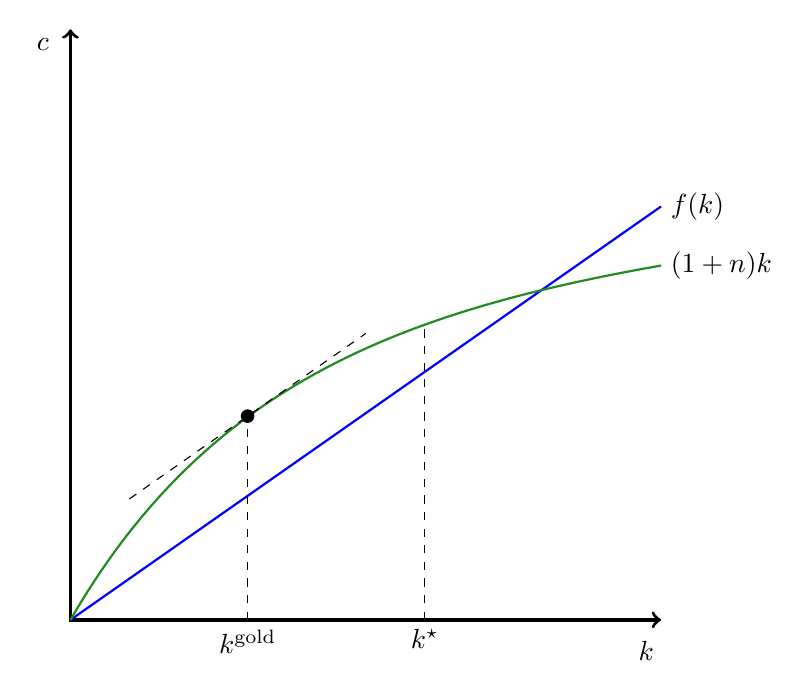
\begin{tikzpicture}[scale=0.75]
		\draw[very thick, <->] (0,10)--(0,0)--(10,0);
		\node[left] at (-0.2,9.75) {$c$};
		\node[below] at (9.75,-0.2) {$k$};
		
		\draw[thick, blue] (0,0)--(10,7);
		\node[right] at (10,7) {$f(k)$};
		\draw[thick, ForestGreen] (0,0) to[out=60,in=190] (10,6);
		\node[right] at (10,6) {$(1+n)k$};
		
		\draw[dashed] (1,2.05)--(5,4.85);
		\filldraw[black] (3,3.45) circle(3pt);
		\draw[dashed] (3,0)--(3,3.45);
		\draw[dashed] (6,0)--(6,5);
		
		\node[below] at (3,0) {$k^\text{gold}$};
		\node[below] at (6,0) {$k\opt$};
	\end{tikzpicture}
	\caption{Golden Rule Capital}
	\label{fig:golden_rule_OLG}
\end{figure}

\begin{definition}
	The economy is \blue{dynamically inefficient} if it involves overaccumulation (\ie if $k\opt > k^{\text{gold}}$). An alternative to this condition is $R\opt < 1 + n \Longleftrightarrow r\opt < n$. Transversality in a standard one-sector growth model requires $r > g + n$, but we do not impose transversality in the OLG model, since agents live for two periods and solve finite problems. 
\end{definition}

\begin{remark}
	Individuals born at time $t$ face prices determined by the stock of capital chosen by the previous generation. Pecuniary externality: actions of the previous generation affect those further on. These typically do not matter for welfare (because they are second order), but these affect an infinite stream of newborn agents. These pecuniary externalities can be exploited, and we will see this in the application.
\end{remark}


\begin{proposition}
	In the baseline OLD, the compaetitive equilibrium is not necessarily Pareto optimal. Whenever $r\opt < n$ the economy is dynamically inefficient. Hence, it is possible to reduce the capital stock in the steady state and increase consumption for all generations.
\end{proposition}
\begin{proof}
	Consider changing next period's capital stock so that $\Delta k < 0$, and then move towards the steady state. This will lead to lower savings in the first period, so $\Delta c_T = (1+n)\Delta k >0$, meaning that everyone is happier. Further, since $k\opt > k^{\text{gold}}$, for small $\Delta k$, \[\Delta c_t = -(f'(k\opt - \Delta k) - (1+n))\Delta k \Longrightarrow f'(k\opt - \Delta k) - (1+n) < 0 \Longrightarrow \Delta c_t > 0 \forall t > T\]
	Thus, we've improved consumption in all future periods, showing a Pareto improvement.
\end{proof}

\begin{remark}
	We can think about two types of systems to deal with dynamic inefficiencies: 
	\begin{enumerate}
		\item Fully funded (social security): Young make contributions to the social security system, which are paid back when they are old
		\item Unfunded (pay-as-you-go): Transfers go directly from the young to the current old
	\end{enumerate}
	Pay-as-you-go discourages savings, so it may lead to a Pareto improvement.
\end{remark}

\begin{example}
	\red{Fully-Funded Social Security} The household's problem is
	\[
	\max_{c^t_t,c^t_{t+1},s_t,d_t} u(c_t^t) + \beta u(c^t_{t+1})
	\]
	subject to 
	\[
	c^t_t + s_t + d_t \le w_t \qquad \text{ and } \qquad c_{t+1}^t \le R_{t+1}(s_t+d_t)
	\]
	The government raises $d_t$ from the young, invests it in the capital stock, and pays it back when they are old. Market clearing for capital requires $s_t + d_t = (1+n)k_{t+1}$, but the household does not necessarily choose $s_t > 0$. If $s_t$ is unconstrained, then given a (feasible) sequence $\{d_t\}_{t=0}^\infty$, the set of competitive equilibria without social security is the set of competitive equilibria with social security if $s_t > 0$. If you impose $s_t \ge 0$ (no borrowing), then a (feasible) sequence $\{d_t\}_{t=0}^\infty$ is a competitive equilibrium if the equilibrium savings is such that $s_t > 0$ for all $t$. This implies that there cannot be a Pareto improvement if we impose $s_t \ge 0$.
\end{example}

\begin{example}
	\red{Unfunded Social Security} The household's problem is 
	\[
	\max_{c^t_t,c^t_{t+1},s_t} u(c_t^t) + \beta u(c^t_{t+1})
	\]
	subject to 
	\[
	c^t_t + s_t + d_t \le w_t \qquad \text{ and } \qquad c_{t+1}^t \le R_{t+1}s_t + (1+n)d_{t+1}
	\]
	The government raises $d_t$ from the young and distributed $(1+n)d_t$ to the old. The rate of return on social security is $1+n$ rather than $R_{t+1}$, and only $s_t$ goes to capital accumulation. 
\end{example}

\begin{remark}
	Unfunded social security reduces capital accumulation! What effect will that have on growth and welfare? If the economy is dynamically inefficient, this may be good... however most poorer countries have capital accumulation that is too low rather than too high. However, social security transfers resources from future generations to the initial old generation. With no dynamic inefficiency, this will make some future generation worse off!
\end{remark}



\subsection{Heterogeneity}

We will talk about heterogeneity and consumption distribution, Gorman aggregation, and variance of consumption. We will typically take income as exogenous, and consider differences in consumption as the objects of interest with respect to the heterogeneity.

\href{https://en.wikipedia.org/wiki/Thomas_Piketty}{Piketty} talked in capital about how capital growth, when wages are stagnant, can lead to increases in inequality. Specifically, recent automation is a large concern here. This is a recent question -- in older history, growth was associated with sharp declines in inequality, rather than increases. Weirdly, inequality in the 20th century seemed to decline until the 1960s, when inequality in the U.S. increased by massive amounts.

\begin{question}
	Is the one-sector growth model consistent with some degree of heterogeneity across households?
\end{question}

Under some conditions, we can show that heterogeneity in initial wealth, effective labor (\ie human capital), and (limited) differences in utility do not affect equilibrium. Why? Because the `averages' remain the same across the economy, which is identical to the representative agent economy. The basic ideas go back to Gorman on aggregation.


\begin{model}
	\red{Heterogeneity} We have $N$ households, each characterized by a vector $(\theta_i,a_i,e_i)$ where $a_i$ are assets and $e_i$ endowments of labor, and individual utility \[u_i(c) = \frac{(c+\theta_i)^\eta}{1-\eta}\]where $\eta > 0$ and $\theta_i$ can be either positive or negative. The household problem is \[\max_{\{c_{i,t},a_{i,t+1}\}} \sum_{t=0}^\infty \beta^t u_i(c_{i,t})\]subject to \[c_{i,t} + a_{i,t+1} \le w_te_i + R_ta_{i,t} \forall t = 0,1,\dots \qquad \text{ and }\qquad \lim_{T\to\infty} \beta^T u'_i(c_{i,T})a_{i,T+1} = u\]with $a_{i,0}$ given. We also have a present value budget constraint, where \[\sum_{t=0}^\infty q_tc_{i,t} \le \sum_{t=0}^\infty q_tw_te_i + q_0a_{i,0} \text{ where } q_t \equiv \prod_{j=1}^t R_j^{-1}\]
	
	The representative firm solves the standard problem \[\max_{c_t,x_t} c_t + p_{kt} x_t - w_te_t - r_tk_t \]subject to \[c_t + x_t = F(k_t,e_t) \qquad \text{ and } \qquad k_{t+1} = (1-\delta)k_t + x_t\]
	
	Let $N$ be the number of households in the economy. For any variable $z_{it}$, let $z_t = N^{-1} \sum_{i\le N} z_{i,t}$, meaning the population average. We have first and second moments (including covariance) as usual, and we define $\theta \equiv N^{-1} \sum_{i=1}^N \theta_i$, $a_t \equiv N^{-1} \sum_{i=1}^N a_{it}$, and $e \equiv N^{-1} \sum_{i=1}^N e_{i}$.
	
	
	\begin{definition}
		A competitive equilibrium is a collection of price sequences $\{q_t,w_t,r_t,R_t\}$, an allocation $\{x_t,k_t,\{c_{it}\}\}$ and a sequence of asset holdings $\{a_{it}\}$ such that
		\begin{enumerate}
			\item Given prices, the allocation and sequence of assets maximizes utility
			\item Given the equilibrium prices, the allocation maximizes profits
			\item The allocation is feasible: market clearing and aggregate law of motion for capital
			\item $a_0 = k_0 > 0$ given
		\end{enumerate}
	\end{definition}
	
	\begin{proposition}
		Average quantities corresponding to a competitive equilibrium also solve the planner's problem: \[\max_{\{c_t,x_t,k_{t+1}\}} \sum_{t=0}^\infty \beta^t \frac{(c_t + \theta)^{1-\eta}}{1-\eta}\]subject to $c_t + x_t \le F(k_t,e_t)$ and $k_{t+1} = (1-\delta)k_t + x_t$.
	\end{proposition}
	\begin{proof}
		Assume an interior solution. Thef irst order condition for the planner's problem is just \[(c_t + \theta)^{-\eta} = \beta(c_{t+1} + \theta)^{-\eta}[1-\delta + F_k(k_{t+1},e_{t+1})]\]The Euler equation for family $i$ is \[(c_{it} + \theta_i)^{-\eta}= \beta(c_{it+1} + \theta_i)^{-\eta} R_{t+1}\]but $R_{t+1} = [1-\delta + F_k(k_{t+1},e_{t+1})]$, which implies that \[(c_{it} + \theta_i)= \beta^{-1/\eta}(c_{it+1} + \theta_i) [1-\delta + F_k(k_{t+1},e_{t+1})]^{-1/\eta}\]Averaging each side, we get\[N^{-1} \sum_{i=1}^N (c_{it} + \theta_i)= N^{-1}\sum_{i=1}^N \beta^{-1/\eta}(c_{it+1} + \theta_i) [1-\delta + F_k(k_{t+1},e_{t+1})]^{-1/\eta}\]
	\end{proof}
	
	\begin{question}
		What are the implications in this model for consumption mobility and cross-sectional dispersion of consumption?
	\end{question}
	If we write the FOC of the household with the present-value budget constraint, we get \[c_{it} + \theta_i)^{-\eta} = \lambda_i \frac{q_t}{\beta^t} \Longrightarrow c_{it} + \theta_i) = \parl \lambda_i \frac{q_t}{\beta^t}\parr^{-1/\eta}\]We can use this expression in the budget constraint to solve for $\lambda_i$:
	\[
	\lambda_i^{-1/\eta} \sum_{t=0}^\infty q_t \parl \frac{q_t}{\beta^t}\parr^{-1/\eta} = e_i \sum_{t=0}^\infty q_tw_t + \theta_i \sum_{t=0}^\infty q_t + q_0 a_{i0}
	\]
	For any sequence $z_t$, let $v(z,q) = \sum_{t=0}^\infty q_tz_t$. Then we have \[\lambda_i^{-1/\eta} v\parl \parl \frac{q_t}{\beta^t}\parr^{-1/\eta},q\parr = e_iv(w,q) + \theta_iv(1,q) + q_0a_{i0}\]Let $\Phi_t = \frac{q_t}{\beta_t}$ and $\Phi_0 = 1$. Then we have \[\lambda_i^{-1/\eta} = \frac{e_iv(w,q) + \theta_iv(1,q) + a_{i0}}{v(\Phi_t^{-1/\eta},q)}\]Using this multiplier in the FOC of the household, we get \[c_{it} = \frac{e_iv(w,q) + \theta_iv(1,q) + a_{i0}}{v(\Phi_t^{-1/\eta},q)}\Phi_t^{-1/\eta}- \theta_i\]Note that consumption for each household is a linear function of $e_i,\theta_i,a_{i0}$. Let $M_i$ be such that \[M_i \equiv m_e e_i+m_\theta\theta_i + m_aa_{i0}\]where $m_e = \frac{v(w,q)}{v(\Phi_t^{-1/\eta},q)} $, $m_\theta = \frac{v(1,q)}{v(\Phi_t^{-1/\eta},q)}$, and $m_a = \frac{1}{v(\Phi_t^{-1/\eta},q)}$. Also, let $M = m_e e + m_\theta \theta + m_a a_0$. Then we have that \[c_{it} = M_i \Phi_t^{-1/\eta} -\theta_i \qquad \text{ and } \qquad c_{t} = M \Phi_t^{-1/\eta} -\theta\]
	\begin{remark}
		Key features here: all individuals face the same prices, aggregate demand functions are independent of the distribution of the personal characteristics, and a necessary and sufficient condition is that the Engel curves be affine.
	\end{remark}
	
	Household $i$'s relative consumption is $c_{it}^R = \frac{c_{it}}{c_t}$.
	
	\begin{proposition}
		The long-run distribution of consumption is non-degenerate (\ie it is not true that as $t \to \infty$, $c_{it}^R = 1$).
	\end{proposition}
	\begin{proof}
		We know that $c_t \to c\opt$, and if $k_0 < k\opt$ then $c_t$ is monotonically increasing. Thus, $\Phi_t^{-1/\eta} \to (\Phi\opt)^{-1/\eta} > 0$ for some $\Phi\opt$, and \[c_i^{R\opt} = \frac{M_i (\Phi\opt)^{-1/\eta} - \theta_i}{M (\Phi\opt)^{-1/\eta} - \theta} \ne 1\]
	\end{proof}
	\begin{question}
		When do we observe $c^{R\opt}_i < 1$? Well, \[c^{R\opt}_i < 1\iff M_i (\Phi\opt)^{-1/\eta} - \theta_i < M (\Phi\opt)^{-1/\eta} - \theta \]which holds if \[(\Phi\opt)^{-1/\eta}\barl m_e (e_i - e) + m_a(a_{i0} - a_0)\barr < (\theta_i - \theta)\parl 1 - (\Phi\opt)^{-1/\eta}m_\theta\parr\]
	\end{question}
	\begin{remark}
		Some comparative statics: higher $e_i$ or $a_{i0}$ leads to higher $c_i^{R\opt}$; lower $\theta_i$ leads to lower $c_i^{R\opt}$. We also have the (painful) second moments: 
		\begin{align*} 
			\sigma^2(c_i^{R\opt}) = \frac{1}{\barl M (\Phi\opt)^{-1/\eta} - \theta_i\barr^2}\Bigg\{ &(\Phi\opt)^{-2/\eta}\barl m_e^2 \sigma^2(e) + m_a^2\sigma^2(a_0)\barr + \parl (\Phi\opt)^{-1/\eta} m_\theta - 1\parr^2\sigma^2(\theta) \\ &+ 2(\Phi\opt)^{-1/\eta}\barl m_em_a\sigma(e,a_0) + (m_\theta-1)(m_e \sigma(e,\theta) + m_a \sigma(a_0,\theta))\barr\Bigg\}
		\end{align*}
		Notice that $\sigma^2(c_i\opt) = \sigma^2(c_i^{R\opt}) \barl M (\Phi\opt)^{-1/\eta} - \theta_i\barr^2$, so even if we have two economies $A$ and $B$ with $\sigma^2_A(e) =\sigma^2_B(e) $ and $\sigma^2_A(a_0) = \sigma^2_B(a_0)$, we will have differences in consumption variance. A positive covariance between any two of the elements that make up a household's type increases long-run variance in consumption. 
	\end{remark}
	\begin{question}
		What do you think of the statement `Controlling for initial wealth inequality, all countries display the same amount of consumption inequality'?
	\end{question}
\end{model}

\begin{model} 
	\red{Bewley Economies} We have that agents are \emph{ex ante} identical, where the only source of heterogeneity is income risk. Agents cannot insure against these shocks due to incomplete markets. We have discrete time and no aggregate uncertainty, so the aggregate endowment $\bar{e}$ is constant. We have a measure 1 of infinitely-lived households, with preferences \[\expect_0 \sum_{t=0}^\infty \beta^t u(c_{it})\]We have random endowments $e_{it} \in E$ where $|E|<\infty$, and transition matrix $\pi(e_{it+1},e_{it})$ with stationary distribution $\Pi(e)$, where $\Pi(e) = $ the measure of households with endowment $e$. The households solve \[\max_{c_{it},a_{it+1}}\expect_0 \sum_{t=0}^\infty \beta^t u(c_{it})\]subject to a budget constraint and a borrowing constraint:\[c_{it} + a_{it+1} = e_{it} + (1+r)a_{it} \qquad \text{ and } \qquad a_{it+1} \ge -b,\text{ where } b \in \reals_+\]In recursive form, we have that \[v(a,e) = \max_c u(c) + \beta \sum_{e'} \pi(e',e)v(a',e')\]subject to \[c + a' = e + (1+r)a \qquad \text{ and } \qquad a' \ge -b\]
	\begin{remark}
		We need to be careful here! The borrowing constraint may bind here.
	\end{remark}
	This Bellman equation becomes \[v(a,e) = \max_{a'} u(e + (1+r)a - a')+ \beta \sum_{e'} \pi(e' \mid e)v(a',e') + \mu(a' + b)\]Sufficient conditions for optimality are\begin{align*}
		\frac{\partial u(c)}{\partial c} &= \beta \sum_{e'} \pi(e' \mid e) \frac{\partial v(a',e')}{\partial a'} + \mu &&(a') \\
		\frac{\partial v(a,e)}{\partial a} &= \frac{\partial u(c)}{\partial c}(1+r) &&(a)\\ \mu(a' + b) &= 0 &&(\text{CS})
	\end{align*}
	The Euler equation is \[\frac{\partial u(c)}{\partial c} \ge \beta \sum_{e'} \pi(e' \mid e) \frac{\partial u(c')}{\partial c'}(1+r)\]with equality whenever $a' > -b$ (\ie when $\mu = 0$). Solutions to the household problem are functions $v(a,e)$, $a'(a,e)$ that satisfy the sufficient conditions, for a given $r$.
	
	Assume shocks are i.i.d. Then consumption and savings decisions depend on the current value of income $x \equiv e + (1+r)a$, and savings are increasing in the current value of income $\partial a' / \partial x > 0$. If $x$ is sufficiently high, choose $a' > -b$ and the Euler equation will hold with equality. If not, choose $a' = -b$ and let the Euler equation be violated. Essentially, current consumption is lower than optimal whenever the constraint binds.
	
	The aggregate state is the joint distribution of assets and endowments $\Phi(a,e)$. In a stationary recursive competitive equilibrium, aggregate quantities and prices are constant over time. 
\end{model}

\begin{definition}
	A \blue{stationary equilibrium} is an allocation and prices such that 
	\begin{enumerate}
		\item Households maximize utility per $v(a,e)$, $a'(a,e)$
		\item Markets clear
		\item $\Phi(a,e)$ is time invariant
	\end{enumerate}

For market clearing, we need aggregate consumption: \[C = \int_a \int_e c(a,e) \Phi(da,de) = \int_0^1 e \Pi(de) = e\]and aggregate assets: \[\int_a \int_e a'(a,e) \Phi(da,de) = 0\](since the households borrow from each other). We define a transition function $Q((a,e),(A,E))$ which denotes the probability (or mass of households) in state $(a,e)$ that transition to state $(a',e') \in (A,E)$ tomorrow -- so \[Q((a,e),(A,E)) = \begin{cases} \sum_{e' \in E} \pi(e'\mid e) &\text{if } a'(a,e) \in A \\ 0 &\text{otherwise} \end{cases}\]Note that $a'$ is determined today. Finally, we have the law of motion for $\Phi$ \[\Phi'(A,E) = \int_e \int_e Q((a,e),(A,E)) \Phi(da,de)\]
\end{definition}

\begin{algorithm}
	To solve for the stationary equilibrium:
	\begin{enumerate}
		\item Given the interest rate, solve for the policy function of the household.
		\item Given the policy function, iterate over the law of motion of the aggregate state until $\Phi' = \Phi$.
		\item Using the stationary distribution, check market clearing.
		\item If aggregate asset positions are positive, lower the interest rate and go back to 1.
		\item If aggregate asset positions are negative, raise the interest rate and go back to 1.
		\item Iterate until market clearing is satisfied.
	\end{enumerate}
\end{algorithm}


\begin{example}
	\href{https://www.sciencedirect.com/science/article/pii/016518899390024M}{Huggett (1993)} used six periods per year, a time discount $\beta = 0.66^{1/6} = 0.993$ per period, CRRA utility, a two-state Markov chain with $y_H = 1$, $y_L = 0.1$, and transition probabilities $\pi(H\mid H) = 0.925$, $\pi( L \mid L) = 0.5$, solved on a grid of borrowing constraints $\bar{a}$. The asset policy was basically linear, with optimal for the high types being almost exactly the $45^\circ$ line, and the low types close to a linear downward shift from them. The consumption policy looked as usual, high types always above low types, with the difference being large when asset levels are low and small when asset levels are high. Finally, excess demand is clearly a decreasing, continuous function of the bond price, and so is an increasing and continuous function of the interest rate.
	
	He additionally assumed complete risk-sharing so $c_{it} = C = Y$, bond price (interest rate) $q \equiv \frac{1}{1+r} = \beta$, and asset dynamics $a_{it+1} = (1+r)(a_{it} + e_{it} - Y)$. He found with low risk-aversion, the risk-free rates were 
	
	\begin{center}
	\begin{tabular}{c|c|c}
		$\bar{a}$ & $r$ & $q$ \\\hline
		$-2$ & $-7.1\%$ & 1.0124 \\
		$-4$ & $2.3\%$ & 0.9962 \\
		$-6$ & $3.4\%$ & 0.9944 \\
		$-8$ & $4.0\%$ & 0.9935 \\
	\end{tabular}
	\end{center}
	So a tighter borrowing constraint (higher $\bar{a}$) led to higher demands for savings $(\uparrow q, \downarrow r)$, and looser borrowing constraint (lower $\bar{a}$) led to lower demands for savings $(\downarrow q, \uparrow r)$, with convergence to complete market equilibrium. With high risk-aversion, the risk-free rates were
	\begin{center}
	\begin{tabular}{c|c|c}
		$\bar{a}$ & $r$ & $q$ \\\hline
		$-2$ & $-23\%$ & 1.0448 \\
		$-4$ & $-2.6\%$ & 1.0045 \\
		$-6$ & $1.8\%$ & 0.9970 \\
		$-8$ & $3.7\%$ & 0.9940 \\
	\end{tabular}
	\end{center}
	Higher risk aversion $\alpha$ leads to higher demand for savings, meaning lower $r$ for all $\bar{a}$.
\end{example}

\begin{example}
	\red{Numerical Tools for Incomplete Markets} We want to solve the problem\[V(a,\varepsilon) = \max_{a',\tilde{c} \ge 0} u(\tilde{c}) + \beta \expect\barl V(a',\varepsilon')\barr\]subject to\begin{align*} \tilde{c} + a' &= w\varepsilon + (1+r)a \\ a' &\ge \underline{a} \\ \varepsilon' &= \rho \varepsilon + \epsilon \\ \epsilon &\sim \text{i.i.d}\end{align*}where $\epsilon$ are errors from the autoregressive process. We will solve this using the \blue{Collocation method}, where we say that $V(a,\varepsilon) \approx B(a,\varepsilon)c$ where $B$ are basis functions and $c$ are \blue{collocation coefficients}. Our objective is to find $\hat{f}$ that minimizes \[\|f-\hat{f}\|_\infty \equiv \sup_{x \in D} |f(x) - \hat{f}(x)|\]where a standard function interpolation would have that $\hat{f}(x,c)$ is a linear combination of polynomials with coefficients $c$, where we choose $c$ to minimize $|f - \hat{f}|$ at a finite number of nodes. The key is our choice of polynomial and nodes. 
\end{example}
\begin{algorithm}
	\red{Collocation Method} 
	\begin{enumerate}
		\item Choose basis functions $b_1(x),\dots,b_n(x)$ \begin{remark}
			$b_n(x) = x^n$ typically a bad idea. Often better are Chebyshev orthogonal polynomials or Splines $k$-th order polynomials spliced together (popular choice for linear models).
		\end{remark}
		\item Choose nodes $x = x_1,\dots,x_n$ \begin{remark}
			Equidistant typically are bad. Chebyshev nodes, the roots of the $n$-th degree Chebyshev polynomial, are optimal.
		\end{remark}
	\end{enumerate}
\end{algorithm}

The Chebyshev polynomial has a certain number of waves, depending on the basis. Equidistant nodes will lead to massive tail errors, as $n$ increases. However, using Chebyshev nodes the approximation error decreases as $n$ increases, and we can get a really good approximation of most smooth functions.

Splines basis functions are basically indicator functions, each has a peak at a certain point among the domain. A nice feature of these is that they are shape-preserving, and can be combined to span basically any function you want. Splines can be non-linear, but linear splines actually tend to do a good job.

\begin{algorithm}
	\red{Collocation Method Computation} 
	\begin{enumerate}
		\item Choose order $n$ of polynomial
		\item Choose $m \ge n$ nodes
		\item Evaluate at nodes $B(x)$ 
		\item Find $c$ using $F = Bc$, then compute $c = B \setminus F$ (where $F$ is also evaluated on $x$). 
	\end{enumerate}
	The nodes $B(x)$ are defined as \[B(x) = \matrixc{b_1(x_1) & b_2(x_1) & \cdots & b_n(x_1) \\b_1(x_2) & b_2(x_2) & \cdots & b_n(x_2) \\ \vdots & \vdots & \ddots & \vdots \\ b_1(x_m) & b_2(x_m) & \cdots & b_n(x_m)}\]If we are approximating a multidimensional function $f(x,y)$, we generate $x$ and $y$ nodes, choose basis functions $b^x_i$, $b^y_i$, and approximate \[F = \sum_{i=1}^{n_x}\sum_{i=1}^{n_y}b_i^x(x)b^y_i(y)c_{ij}\]Finally, we find $c$ with $c = B \setminus F$, where $B = B_m \otimes B_{m-1} \otimes \cdots \otimes B_1$.
\end{algorithm}

Back to the incomplete markets model, we will discretize the shock process and solve it using the collocation method, where $V(a,\varepsilon) \approx B(a,\varepsilon)c$. Commonly, people use Tauchen or Rouwenhorst to do this discretization. A common assumption is that $\epsilon \sim \normal(0,\sigma^2)$. In broad strokes, we will:
\begin{enumerate}
	\item Choose the parameters and grid
	\item Define the space, meaning $B$ and $B^E$ \begin{remark} Note that $B^E$ can be computed using $B$ and $c$: \[\expect[V(a,\varepsilon)] = B(a,\varepsilon)c_E = \sum_{\omega_i} \omega_i V(a,\rho \varepsilon + \epsilon_i)= \sum_{\omega_i} \omega_iB(a,\rho \varepsilon + \epsilon_i)c \Longrightarrow c_E = \underbrace{B(a,\varepsilon)^{-1}\sum_{\omega_i} \omega_iB(a,\rho \varepsilon + \epsilon_i)c}_{B^E}\]	\end{remark}
	\item Then we guess $c_0$ and solve the following linear equation until convergence: \[B(a,\varepsilon)c_{j+1} = \max_{a' \ge 0} u(w\varepsilon + (1+r)a-a') + (a',\varepsilon)B^Ec_j\]
\end{enumerate}


Aggregate assets are $A = \sum_\varepsilon a \cdot\phi(a,\varepsilon)$, and we will assume $A = K$ in equilibrium, and find $r$ such that markets clear. To aggregate we need to compute the \blue{Transition Probability Matrix (TPM)} $P$ using the policy functions. We have a complete ergodic distribution $\phi(a,\varepsilon)$ such that $P$ is a fixed point: $\phi(a,\varepsilon)P = \phi(a,\varepsilon)$. We can solve it by computing the TPM and fining the eigenvectors.

\begin{remark}
	A quick detour on Markov processes. A stochastic process is a sequence of random vectors, indexed by time. A stochastic process has the \blue{Markov property} if for all $t$ and $k \ge 1$,\[\prob(x_{t+1} \mid x_t,\dots,x_{t-k}) = \prob(x_{t+1} \mid x_t)\]Assuming the Markov property, we can characterize a process by a \blue{Markov chain}, where $\pi_0$ is the initial distribution, $P$ is the transition matrix where \[P_{ij} = \prob(x_{t+1}=e_j \mid x_t = e_i),\qquad \sum_{j}P_{ij} = 1\]and $e_i$ is a vector of zeros except for 1 in entry $i$. The probability of being in state $j$ in two periods is:\[P_{ij}^2 = \prob(x_{t+2} = e_j \mid x_t = e_i) = \sum_{h=1}^n \prob(x_{t+2} = e_j \mid x_{t+1} = e_h)\prob(x_{t+1} = e_h \mid x_{t+1} = e_i)\]Therefore, unconditional probabilities are determined by \[\pi_1' = \prob(x_1) = \pi_0'P\qquad \text{ and } \qquad \pi_2' = \prob(x_2) = \pi_0'P^2\]A \blue{stationary distribution satisfies} $\pi' = \pi' P \Longrightarrow \pi'(I-P) = 0 \Longrightarrow (I-P')\pi = 0$. Does this distribution necessarily exist? Yes! $P$ has at least one eigenvalue and at least one eigenvector $\pi$, which we can normalize such that $\sum_i \pi_i = 1$. Multiplicity is possible, however. For a given $\pi_0$, it might be the case that \[\lim_{t\to\infty} \pi_t = \pi_\infty\]If this equation holds and $\pi_\infty \indep \pi_0$, then the process is asymptotically stationary with a unique distribution $\pi_\infty$, called the \blue{asymptotic} (or \blue{invariant}) distribution of $P$.
\end{remark}

\begin{remark}
	Some examples that are interesting to work through:\footnote{CompEcon is very flexible and has some very handy computational tools!}
	\begin{enumerate}
		\item Discrete and continuous choice problems
		\item Heterogeneous firm models
		\item Panel simulations: \begin{enumerate} \item We can also simulate many households over time \item For example: Select a very long period of time and $N$ agents, draw $\varepsilon$ many times, use the policy function to compute the consumption and assets of each agent, for initial conditions to remain irrelevant, remove the first periods of the simulations, and the simulation can either be discrete or continuous. \item We can study micro behavior of consumption and income jointly, checking if the distribution converges to to the one we compute by inverting the TPM, etc  \item Further notes on how to do this in the slides.\end{enumerate}
	\end{enumerate}
\end{remark}

\subsection{Continuous Time Growth}

Some facts about continuous time growth (assuming that production technology is Cobb-Douglas, where $Y_t = A_tM_tK_t^\alpha H_t^{1-\alpha}$ for $H_t$ human capital, $M_t$ is a measure of uncertainty, and $A_t$ is the level of technology):
\begin{enumerate}
	\item Mathematically, we have that \[\frac{Y_t}{L_t} = Z_t \frac{H_t}{L_t}\parl \frac{K_t}{Y_t}\parr^{\frac{\alpha}{1-\alpha}} \qquad \text{ and } \qquad Z_t = (A_tM_t)^{\frac{1}{1-\alpha}}\] So all long-term growth in the Ramsay-Cass-Koopmans model is from either $A$ or population $L$, which is exogenous!
	\item From the one-sector growth model, we have that (i) $\frac{Y_t}{L_t}$ and $\frac{K_t}{L_t}$ grow over time at roughly constant equal rates (implication: $\frac{K_t}{Y_t}$ constant over time), (ii) that $\frac{I_t}{Y_t}$ is constant, and (iii) that $\frac{R_tK_t}{Y_t}$ and $\frac{W_tL_t}{Y_t}$ constant.
	\item These predictions are consistent with the Kaldor facts!
	\item They also are consistent with \emph{some} catch-up dynamics, but transitions are too fast.
\end{enumerate}

\begin{model}
	\red{Ramsay-Cass-Koopmans (RCK)} We have a representative, infinitely-lived family (or dynasty), with population growth $n > 0$, labor force $L(t) = \exp(nt)$ where $L(0) =1$ by assumption, constant returns technology $Y(t) = F(K(t),A(t)L(t))$, and capital dynamics: \[\dot{K}(t) + \delta K(t) = F(K(t),A(t)L(t)) - C(t)\]define $c_t = \frac{C(t)}{L(t)}$, $\zeta(t) = \frac{C(t)}{A(t)L(t)}$, and $\kappa(t) = \frac{K(t)}{A(t)L(t)}$ (this is in \blue{efficiency units}). We have that \[\frac{\dot{K}(t)}{A(t)L(t)} + \frac{\delta K(t)}{A(t)L(t)} = F\parl \frac{K(t)}{A(t)L(t)},1\parr - \frac{C(t)}{A(t)L(t)}\]which simplifies to \[\dot{\kappa}(t) = F(\kappa(t)) - \zeta(t) - (n + g + \delta)\kappa(t)\]and thus \[\dot{\kappa}(t) =\parl \dot{\frac{K(t)}{A(t)L(t)}}\parr = \frac{\dot{K}(t)}{A(t)L(t)} - n\kappa(t) - g\kappa(t)\]
	Note the intuition here: we have that $\frac{1}{A(t)} \frac{\partial A(t)}{\partial t} = g$, and that $\frac{1}{L(t)} \frac{\partial L(t)}{\partial t} = n$. We can show this by using Ekaterina's trick of converting to logarithmic forms, taking derivatives, and showing that those partials are equivalent to the (more complicated) fractions.
	
	Problem: $F$ is decreasing in capital, meaning no endogenous long-run growth!
	
	Solution: Constant returns to capital! See below.
\end{model}

\begin{model}
	\red{The AK Model.} The simplest version of this assumes that $Y(t) = A(t)K(t)$, capital per capital is $\frac{K(t)}{L(t)}$, and feasibility is \[\dot{k}(t) = Ak(t) - c(t) - \delta k(t)\]or, with population growth,\[\dot{k}(t) = Ak(t) - c(t) - (n+\delta)k(t)\]The family values \emph{per capita} consumption as\[u(c) = \int_0^\infty \exp(-\rho t)U(c(t))dt\]where $\rho$ is the time discount factor, and $U(c(t))$ is a CRRA function, so $U(c) = \frac{c^{1-\sigma}}{1-\sigma}$. We can show that an allocation $(k,c)$ is Pareto optimal if and only if it solve the social planner's problem, which is \[\max_{k,c \ge 0} \int_0^\infty \exp(-\rho t) U(c(t))dt \]subject to \[\dot{k}(t) = Ak(t) - c(t) - (n+\delta)k(t)\qquad \text{ with } \qquad k(0) =k_0\]We can solve this problem using Pontryagin's Maximum Principle, with control variable $c$, state variable $k$, and co-state variable $\lambda$. The present-value Hamiltonian is\[\mathcal{H}(t,k,c,\lambda) = \exp(-\rho t) U(c(t)) + \lambda(t) \barl f(k(t)) - c(t) - (n+\delta)k(t)\barr\]which admits sufficient conditions \begin{align*} 0 &= \exp(-\rho t)U'(c(t)) -\lambda(t) &&(c) \\ \dot{\lambda}(t) &= -\barl f'(k(t))- (n+\delta)\barr \lambda(t) &&(k) \\ 0 &= \lim_{t\to\infty} \lambda(t)k(t) &&(TVC)\end{align*}plus the constraint \[\dot{k}(t) = Ak(t) - c(t) - (n+\delta)k(t)\]We can get rid of the co-state variable by differentiating \[\dot{\lambda}(t) = \exp(-\rho t)U''(c(t))\dot{c}(t) - \rho \exp(-\rho t)U'(c(t)) \Longrightarrow \frac{\dot{\lambda}(t)}{\lambda(t)} = \frac{U''(c(t))}{U'(c(t))	} \dot{c}(t) - \rho\]where we replace \[-\barl f(k(t))-(n+\delta + \rho)\barr c(t) = \frac{U''(c(t))}{U'(c(t))}c(t)\dot{c}(t)\]and because $U$ is CRRA,\[\sigma \dot{c}(t) = \barl A - (n + \delta + \rho)\barr c(t)\]
\begin{definition}
	A \blue{balanced growth path (BGP)} is an allocation such that consumption, capital, and output grow at a constant (possibly different) growth rate\[\frac{\dot{x}(t)}{x(t)} = \gamma_x > 0 \text{ for any variable } x\]
\end{definition}
	In this particular problem, the consumption dynamics are independent of capital:\footnote{Note not true in the standard RCK model, remember the sequential economy.}\[c(t) = \exp\parl \frac{1}{\sigma} \barl A - (n + \delta + \rho)\barr t\parr c(0)\]So consumption grows at a constant rate from the beginning. Capital dynamics are \[\frac{\dot{k}(t)}{k(t)} = A - \frac{c(t)}{k(t)} - (n + \delta)\]Along the BGP, consumption and capital grow at the same rate, so the economy is on the BGP from time $t=0$. We need an additional condition so that utility does not blow up, so $U$ remains well-defined. Observe that:\[\int_0^\infty \exp(-\rho t) U(c(t))dt = c(0)^{\frac{1-\sigma}{\sigma}} \int_0^\infty \exp(-\rho t)\frac{\exp\parl \frac{1-\sigma}{\sigma}\barl A - (n + \delta + \rho)\barr t\parr dt}{1-\sigma}\]So we need that \[\frac{1-\sigma}{\sigma} \barl A - (n+\delta) - \frac{\rho}{1-\sigma}\barr < 0\]
	\begin{remark}
		The main implication is that no country can ever catch up. However, we see some of that in the data -- how do we reconcile that? What would happen if we added labor? With increasing returns to scale, we don't have a well-defined equilibrium in the standard AK model. \href{https://econpapers.repec.org/article/ucpjpolec/v_3a94_3ay_3a1986_3ai_3a5_3ap_3a1002-37.htm}{Romer (1986)} argued for increasing returns to scale but the agents in the economy behave as if constant returns to scale.
	\end{remark}
\end{model}

\begin{question}
	Why do we consider discounting rather than no discount factor and maximize mean consumption in each period rather than have discounting?
\end{question}
\begin{answer}
	We don't exactly have a Permanent Income Hypothesis here, as this is a production economy. We essentially, in most cases, have a single optimal path, and it's always worth it to get on the optimal path as quickly as possible. See \href{https://en.wikipedia.org/wiki/Turnpike_theory}{the Turnpike Theorem}.
\end{answer}

\begin{model}
	\red{RCK with Productivity Growth} Recall that the optimal allocation satisfies \begin{align*} \dot{\zeta}(t) &= \frac{1}{\sigma} \barl f'(\kappa(t)) - (n + \sigma g + \delta + \rho)\barr \zeta(t) \\ \dot{\kappa}(t) &= f(\kappa(t)) - \zeta(t) - (n + g + \delta)\kappa(t) \\0 &= \lim_{t\to\infty} \exp(-\hat{\rho}t) U'(\zeta(t))\kappa(t) \end{align*}where $g$ is exogenous growth of technology, and $\kappa(t) = \frac{K(t)}{A(t)L(t)}$, $\zeta(t) = \frac{C(t)}{A(t)L(t)}$. We have steady state analysis $x\opt = (\zeta\opt ,\kappa\opt)$, and saddle paths. From the theory of linear approximation, we know that when the path is ``nice'' (this condition is quite important! think of it as a convex problem that is everywhere differentiable), the behavior around the steady state is well-approximated by the behavior of a linear system around the steady state. We use the first-order Taylor approximation \[f(x) = f(x\opt) + \nabla f(x\opt) \cdot (x-x\opt)\]where $\nabla f(x\opt)$ is the $\reals^n$ gradient to $f$ at $x\opt$. In our case, $x\opt = (\zeta\opt,\kappa\opt)$ and we have $g_1$ and $g_2$ that solve 
	\begin{align*}
		g_1(\zeta(t),\kappa(t)) = \dot{\zeta}(t) &= \frac{1}{\sigma} \barl f'(\kappa(t)) - (n + g + \delta + \rho)\barr \zeta(t) \\ g_2(\zeta(t),\kappa(t)) = \dot{\kappa}(t) &= f(\kappa(t)) - \zeta(t) - (n + g + \delta)\kappa(t)
	\end{align*}
	where $g_1(\zeta\opt,\kappa\opt) = g_2(\zeta\opt,\kappa\opt) = 0$. From our linear approximation, we have 
	\[
	\matrixc{\dot{\zeta}(t) \\ \dot{\kappa}(t)} \approx \matrixc{ -\frac{1}{\sigma}[f'(\kappa(t)) - (n + g + \delta+ \rho)] & -\frac{1}{\sigma} f''(\kappa(t))\zeta(t) \\ -1 & f'(\kappa(t)) - (n+g+\delta) }_{(\zeta\opt,\kappa\opt)} \matrixc{ \zeta(t) - \zeta\opt \\ \kappa(t) - \kappa\opt}
	\] 
	which becomes 
	\[
	\matrixc{\dot{\zeta}(t) \\ \dot{\kappa}(t)} \approx \matrixc{0 & -\frac{1}{\sigma} f''(\kappa\opt)\zeta\opt \\ -1 & \rho }_{(\zeta\opt,\kappa\opt)} \matrixc{ \zeta(t) - \zeta\opt \\ \kappa(t) - \kappa\opt}
	\]
	This is a two-dimensional difference equation that can be solved analytically. We look at the eigenvalues of $\nabla f(\zeta\opt,\kappa\opt)$, $\lambda$, which satisfy \[ 0 = \det(\nabla f(\zeta\opt,\kappa\opt)-\lambda I) = -\lambda(\rho - \lambda) + \frac{1}{\sigma} f''(\kappa\opt)\zeta\opt\]This quadratic equation has two roots, one negative and one positive. Let $l$ be the number of negative eigenvalues, and let $m$ be the number of state variables of the problem. Stability comes directly from these: if $l = m$, we are \blue{saddle-path stable}, we have a unique optimal trajectory (the negative eigenvalue governs the speed of convergence), if $l < m$, unstable, no convergence to the steady state, and if $l > m$, indeterminacy, multiple optimal trajectories.
	
	The speed of convergence is \[\kappa(t) - \kappa\opt \approx e^{-|\lambda_1|t}(\kappa(0) - \kappa\opt)\]with half-life\[\kappa(t_{1/2})-\kappa\opt \approx \frac{1}{2} (\kappa(0) - \kappa\opt) \text{ hence } t_{1/2} = \frac{\ln(2)}{|\lambda_1|}\]
\end{model}


\subsection{Endogenous Growth Theory}

\subsubsection{Externalities}

The AK model generates long-term growth. Typically, we think about this as either spillovers or learning by doing. How do we endogenize growth?


	
	\begin{remark}
		First, what worked in the AK model? Constant returns in a reproducible factor (capital), and we left out the non-reproducible factor (labor). The dilemma is that we left out the non-reproducible factor. Paul Romer had an elegant solution.
	\end{remark}
\begin{model}
	\red{Endogenous Growth Model} (from \href{https://extranet.parisschoolofeconomics.eu/docs/darcillon-thibault/paul-romer-increasing-returns-and-long-run-growth.pdf}{Romer (1986)}) The economy is the same as the AK model setup but we have a continuum of firms that produce output with technology \[y_i(t) = F(k_i(t),l_i(t)K(t))\]where firms are indexed with $i \in [0,1]$, $k_i,l_i$ are capital and labor at firm $i$, $K(t) = \int k_i(t)di$ is aggregate capital, and $F(\cdot)$ has constant returns to scale with respect to $k_i$ and $l_i$. This gives us an externality, where firms do not understand that requesting more capital will increase the aggregate capital, they just take that as given.\footnote{This is often called the \blue{Big $K$ / small $k$ model}.} The firm's problem is \[\max_{k_i,l_i} F(k_i(t),l_i(t)K(t)) - w(t)l_i(t) - r(t)k_i(t)\]where $K(t)$ is \blue{exogenous to the firm}. Note that there are increasing returns to scale overall: \[F(\theta k_i(t),\theta l_i(t)\underbrace{\theta K(t)}_{=\int \theta k_i(t)di}) = F(\theta k_i(t),\theta^2 l_i(t) K(t)) > \theta F( k_i(t), l_i(t) K(t))\]for any $\theta > 1$. The competitive equilibrium exists in this economy because from the firm's perspective there are constant returns to scale. Will it be Pareto Optimal? Not in general! This is straightforward to see, in a world with externalities. 
	
	As before, the households are a size $L$ of identical people, with no population growth.
	
	\begin{definition}
		A \blue{competitive equilibrium} is a set of allocations $\{\hat{c}(t),\hat{a}(t)\}$ for the representative household, a set of allocations $\{\hat{k}_i(t),\hat{l}_i(t)\}$ for each firm $i$, a stream of aggregate capital stock $\{\hat{K}(t)\}$, and a stream of prices $\{\hat{w}(t), \hat{r}(t)\}$ such that:
		\begin{enumerate}
			\item Given prices, $\{\hat{c}(t),\hat{a}(t)\}$ solves \[\max_{\{c(t),a(t)\}} \int \exp(-\rho t) \frac{c(t)^{1-\sigma}}{1-\sigma}dt \] subject to \begin{align*} c(t) + \dot{a}(t) + a(t) &= w(t) + (r(t)-\delta)a(t) \\ a(0) &= k(0) \text{ given} \\\lim_{t\to\infty} a(t)\exp \parl - \int_0^t (r(\tau)-\delta)d\tau\parr &\ge 0 \end{align*}
			\item Given $\{\hat{w}(t), \hat{r}(t)\}$ and $\{\hat{K}(t)\}$, the path $\{\hat{k}_i(t),\hat{l}_i(t)\}$ maximizes firm profits in each period for each firm
			\item Feasibility: for all $t$, markets clear: \[L\hat{c}(t) + \dot{\hat{K}}(t) + \hat{K}(t)\delta = \int_0^1 F(\hat{k}_i(t) , \hat{l}_i(t) \hat{K}(t)) di\]\[\int_0^1 \hat{l}_i(t)di = L \qquad \text{ and } \qquad \int_0^1 \hat{k}_i(t)di = L\hat{a}(t)\]
			\item Rational Expectations: \[\int_0^1 \hat{k}_i(t)di = \hat{K}(t)\]
		\end{enumerate}
	\end{definition}
	
	The planner's problem is \[\max_{c(t),K(t)} \int \exp(-\rho t) \frac{c(t)^{1-\sigma}}{1-\sigma} dt \]subject to\[Lc(t) + \dot{K}(t) - K(t) \delta = F(K(t) ,LK(t)) \text{ with } K(0) = Lk(0)\]Note that the planner can deal in terms of total capital and total labor, because the firms have identical production functions, so when they choose capital and labor so that the marginal products of capital and labor respectively equal the wage and rental price, they all choose the same levels, so they can be aggregated. The planner can choose first the aggregates and next how to split them across the agents. Optimality requires that \[\gamma_C^{SP}(t) = \frac{\dot{c}(t)}{c(t)} = \frac{1}{\sigma} \Big[ F_1(K(t),LK(t)) + F_2(K(t),LK(t))L - (\delta + \rho)\Big]\]Since $F$ is homogeneous of degree 1 in capital, $F'$ is homogeneous of degree 0, so we have that \[F_1(K(t),LK(t)) + F_2(K(t),LK(t))L = F_1(1,L) + F_2(1,L)L\]Thus, consumption growth is\[\gamma_C^{SP}(t) = \frac{\dot{c}(t)}{c(t)} = \frac{1}{\sigma} \Big[F_1(1,L) + F_2(1,L)L - (\delta+\rho)\Big]\]which is constant in time! From the aggregate resource constraint:\[L \frac{c(t)}{K(t)} + \frac{\dot{K}(t)}{K(t)} + \delta = F(1,L)\]so in the balanced growth path, $\gamma_C^{SP}(t) = \gamma_k^{SP}(t) = \gamma_K^{SP}(t)$. From the first order conditions of the household and the firm, we have that \[\gamma_C^{CE}(t) = \frac{\dot{c}(t)}{c(t)} = \frac{1}{\sigma}\Big[ r(t) - (\delta + \rho)\Big] \quad \text{ and } \quad r(t) = F_1(k_i(t),l_i(t)K(t)) \]Since all firms are identical and choose the same allocations, $k_i(t) = k(t) = \int k_i(t) di = K(t)$ and $l_i(t) = L$, so $r(t) = F_1(1,L)$, so\[\gamma_C^{CE}(t) = \frac{1}{\sigma} \Big[F_1(1,L) - (\delta+ \rho)\Big]< \gamma_C^{SP}(t)\]since $F_2(1,L) > 0$. So in the balanced growth path, $\gamma_C^{CE} = \gamma_k^{CE} = \gamma_K^{CE}$. How do we bring $\gamma_K^{CE}$ to $\gamma_K^{SP}$? With a subsidy per unit of capital invested, equal to $F_2(1,L)L$. That will make the cost of capital to the firms $r(t) - F_2(1,L)L$.
	\end{model}
	\begin{remark}
		A prediction of this model is that larger economies grow more, where \[\gamma_C^{CE}(t) = \frac{\dot{c}(t)}{c(t)} = \frac{1}{\sigma} \barl F_1(1,L)- (\delta + \rho)\barr < \gamma_C^{SP}(t)\]since $\frac{\partial F(1,L)}{\partial L}> 0$. If $L$ is defined as the labor force of a country (or population), the data across post-World War II countries show no evidence of this fact. Technically, this is because we have constant returns in $K$ and increasing returns in $K$ and $L$. We can avoid this by assuming that productivity depends on the ratio $\frac{K}{L}$ rather than the aggregate. An example of this is the following:
	\end{remark}

\begin{model}
	\red{Externalities in Human Capital} (from \href{https://www.sciencedirect.com/science/article/pii/0304393288901687}{Lucas, 1988}) We have households with measure 1 and human capital $h_i$ for $i \in (0,1)$, with $h_i(0)=h_0$ and $k_i(0) = k_0$. The household chooses time to work $1-s_i(t)$ and time to accumulate human capital $s_i(t)$, with budget constraint(s)
	\begin{align*}
		c_i(t) + \dot{a}_i(t) &= (r(t)-\delta)a_i(t) + (1-s_i(t))h_i(t)w(t) \\
		\dot{h}_i(t) &= \theta h_i(t)s_i(t) - \delta h_i(t)
	\end{align*}
	and production technology \[Y(t) = AK(t)^\alpha L(t)^{1-\alpha}H(t)^\beta\]Firms choose capital and labor and they take $H(t)$ as given. Since the total supply of labor is $(1-s(t))H(t)$, this becomes \[AK(t)^\alpha H(t)^{1-\alpha}H(t)^\beta (1-s(t))^{1-\alpha} = AK(t)^\alpha H(t)^{\beta+ (1-\alpha)}(1-s(t))^{1-\alpha}\]The planner's problem is \[\max \int_0^\infty \exp(-\rho t) \frac{c(t)^{1-\sigma}}{1-\sigma} dt\]subject to\begin{align*} C(t) + \dot{K}(t) + \delta K(t) &= AK(t)^\alpha H(t)^{\beta+ (1-\alpha)}(1-s(t))^{1-\alpha} \\ \dot{H}(t) &= \theta H(t)s(t) - \delta H(t)\end{align*}with $H(0)$ and $S(0)$ given, $s(t) \in [0,1]$, and we have used the fact that \[\int(1-s_i(t))h_i(t) di = L(t) \qquad ; \qquad \int a_i(t)di = K(t) \qquad ; \qquad \int c_i(t) di = C(t)\]Firms solve the simple \[\max_{L(t),K(t)} Y(t) - w(t)L(t) - r(t)K(t)\]where \[r(t) = \alpha \frac{Y(t)}{K(t)} \qquad \text{ and } \qquad w(t) = (1-\alpha) \frac{Y(t)}{(1-s)H(t)}\]Households solve the Hamiltonian
	\begin{align*}
		\mathcal{H}(\cdot) = \exp(-\rho t) \frac{c_i(t)^{1-\sigma}}{1-\sigma} &+ \lambda(t)\barl (r(t)-\delta)a_i(t) + (1-s_i(t))h_i(t)w(t) - c_i(t)\barr \\ &+ \mu(t) \barl \theta h_i(t)s_i(t) - \delta h_i(t)\barr
	\end{align*}
	Again, we have that $\gamma_C^{SP} > \gamma_C^{CE}$.
\end{model}



\subsubsection{Innovation}

In the economies we've studied so far, we've been on the balanced growth path from the beginning. We can think of transition dynamics by relaxing that, and think of growth through variety innovation. 

\begin{model}
	\red{Transition Dynamics} (from \href{https://www.journals.uchicago.edu/doi/abs/10.1086/261717}{Jones \& Manuelli, 1990}) We have production technology\[Y = F(K,L) = AK + BK^\alpha L^{1-\alpha}\]so that $y = Ak + Bk^\alpha$ and $\lim_{t\to\infty} f'(k) = A$. We have growth rates\[\frac{\dot{k}}{k} = \frac{f(k)}{k} - \frac{c}{k} - (n + \delta) \qquad \text{ and } \qquad \frac{\dot{c}}{c} = \frac{1}{\theta} \parl A + B\alpha k^{\alpha-1}- (\rho + \delta)\parr\]where $\theta$ is the elasticity of substitution in consumption. In the balanced growth path, we have growth rates \[\gamma\opt = \frac{1}{\theta} \parl A - (\rho + \delta)\parr\]The problem is that we have no steady state. We can rewrite the variables in stationary terms (\ie \blue{detrend} them). Which variables do we detrend with respect to? Here, capital. Generally it depends on the problem. We have\[z = \frac{f(k)}{k} \qquad \text{ and } \qquad \chi = \frac{c}{k}\]By doing a bunch of (annoying) algebra, we can rewrite the dynamic system as\begin{align*} \dot{z} &= - (1-\alpha)(z-A)(z-\chi - n - \delta) \\ \dot{\chi} &= \chi \parl (\chi - \varphi) - \frac{\theta - \alpha}{\theta}(z-A)\parr \end{align*}where $\varphi \equiv (A-\delta)\frac{\theta-1}{\theta} + \frac{\rho}{\theta} - n$. We can now draw a phase diagram in $(\chi,z)$ space!
\end{model}

\paragraph{Writing Recursively.} (\red{Hamilton-Jacobi-Bellman Equations}) We have \[V(k_0) = \max_{c(t)} \int_0^\infty \exp(-\rho t) U(c(t))dt\]subject to\[\dot{k}(t) = F(k(t)) - \delta k(t) - c(t)\]for $t\ge 0$, with $k(0)=k_0$ given. Our state $x$ is $k(t)$, and the control $u$ is $c(t)$. Let $h(x,u) = U(u)$ and $g(x,u) = F(x) - \delta x - u$. The value function of the generic optimal control problem solves the Hamilton-Jacobi-Bellman equation \[\rho V(x) = \max_u h(x,u) + V'(x)g(x,u)\]With multiple states, $V'(x)$ is a vector of dimension $m$. This implies that \[\rho V(k) = \max_{c} U(c) + V'(k) \barl F(k) - \delta k - c\barr \Longleftrightarrow U'(c) = V'(k)\]We define a discount factor $\beta(\Delta) = \exp(-\rho \Delta)$, where $\Delta$ is the length of a period. We multiply all of our flows by $\Delta$, and keep the stocks the same. The Bellman equation is \[V(k_t) = \max_{c_t} \Delta U(c_t)  + \exp(-\rho\Delta)V(k_{t+\Delta})\]subject to\[k_{t+\Delta} = \Delta[F(k_t) - \delta k_t - c_t] + k_t\]For small $\Delta$, $\exp(-\rho \Delta) \sim (1-\rho \Delta)$, so \[\rho \Delta V(k_t) = \max_{c_t} \Delta U(c_t) + (1-\rho\Delta)(V(k_{t+\Delta}) - V(k_t))\]and so\[\rho V(k_t) = \max_{c_t}U(c_t) + (1-\rho\Delta) \parl \frac{V(k_{t+\Delta}) - V(k_t)}{k_{t+\Delta} - k_t} \frac{k_{t+\Delta} - k_t}{\Delta}\parr\]and taking the limit as $\Delta \to 0$, we get \[\rho V(k_t) = \max_{c_t} U(c_t) + V'(k_t) \dot{k}_t\]Recall that we have had the two general forms:
\[
\underbrace{\mathcal{H}(x,u,\lambda)\equiv h(x,u) + \lambda g(x,u)}_{\text{Hamiltonian}} \qquad ; \qquad \underbrace{\rho V(x) = \max_u h(x,u) + V'(x)g(x,u)}_{\text{Bellman}}
\]
so we can directly see that $\lambda(t) = V'(x(t))$, the co-state variable is the shadow value of the future. Thus:\[\rho V(x) = \max_{u \in U} \mathcal{H}(x,u,V'(x))\]we get the reason for the `Hamilton' in the name of this subsection!


\begin{model}
	\red{Endogenous Technological Change} (from \href{https://web.stanford.edu/~klenow/Romer_1990.pdf}{Romer, 1990}) We can think about expanding input varieties, where a greater variety of inputs increases the `division of labor' which raises the productivity of final goods firms. We have competitive markets for final goods, monopolistic competition for intermediate goods, and competitive markets for R\&D. We have final goods, produced by:\[Y(t) = L(t)^{1-\alpha} \parl \int_0^{A(t)}x_i(t)^{1-\mu}di\parr^{\frac{\alpha}{1-\mu}}\]where $1/\mu$ is the elasticity of substitution. We are interested in $\mu \in (0,1)$, meaning that there is \emph{some} substitution. We also have intermediate goods, produced by\[x_i(t) = al_i(t)\]and R\&D, with constant returns to scale:\[\dot{A}(t) = bX(t)\]where $X(t)$ are final goods devoted to R\&D. We normalize the population to 1, and the planner's problem is
	\[\max \int_0^\infty \exp(-\rho t) \frac{c(t)^{1-\sigma}}{1-\sigma} dt\]subject to \begin{align*}
		c(t) + X(t) &= L(t)^{1-\alpha} \parl \int_0^{A(t)}x_i(t)^{1-\mu}di\parr^{\frac{\alpha}{1-\mu}}\\
		x_i(t) &= al_i(t)\\
		\dot{A}(t) &= bX(t) \\
		L(t) + \int_0^{A(t)}l_i(t)di = 1
	\end{align*}
	Given that there is imperfect substitution, the optimal planner strategy is \[x_i(t) = x(t) \qquad \text{ and } \qquad l_i(t) = l(t)\]Hence,\[c(t) + X(t) = L(t)^{1-\alpha} \parl A(t)(al(t))^{1-\mu}\parr^{\frac{\alpha}{1-\mu}}\]Feasibility requires that $l(t) = \frac{1-L(t)}{A(t)}$, and equilibrium aggregate output is \[Y(t) = a^\alpha L(t)^{1-\alpha} (1-L(t))^\alpha A(t)^{\frac{\alpha\mu}{1-\mu}}\]Output maximization implies that $L(t) = 1-\alpha$. The planner's problem is \[\max \int_0^\infty e^{-\rho t} \frac{c(t)^{1-\sigma}}{1-\sigma}dt  \qquad \st c(t)+\frac{\dot{A}(t)}{b} = CA(t)^{\frac{\alpha\mu}{1-\mu}}\]where $C = a^\alpha (1-\alpha)^{1-\alpha}\alpha^\alpha$. If $\frac{\alpha\mu}{1-\mu} \in (0,1)$, we have Ramsey-Cass-Koopmans. Romer requires that $\alpha\mu = 1-\mu$, so we have an AK model where \[\frac{\dot{c}(t)}{c(t)} = \frac{1}{\sigma}\barl bC - \rho\barr\]so we are on the balanced growth path from the beginning. 
	
	Alternatively, we could solve the decentralized economy. When a new idea is introduced, the R\&D sector charges $k(t)$, where since the sector is competitive and has CRS technology, so $\pi_{R\&D} = 0$. We will assume that $k(t)$ is the present value of the profits of the monopolistic firm, and let $p_i(t)$ be the price of intermediate goods, $p(t)$ be the price of final goods, and $w(t)$ the cost of labor. The final goods firms maximize profits, so we attain the first order conditions 
	\begin{align*}
		w(t) &= (1-\alpha)p(t)L(t)^{-\alpha} \parl \int_0^{A(t)}x_i(t)^{1-\mu}di\parr^{\frac{\alpha}{1-\mu}} &&(L(t)) \\
		p_i(t) &= \alpha p_tL(t)^{1-\alpha} \parl \int_0^{A(t)} x_i(t)^{1-\mu} di \parr^{\frac{\alpha}{1-\mu} - 1}x_i(t)^{-\mu} &&(x_i(t))
	\end{align*}
	which simplify to
	\[w(t) = (1-\alpha)p(t)\frac{Y(t)}{L(t)} \qquad \text{ and } \qquad x_i(t)^\mu = \alpha \frac{p(t)}{p_i(t)}\frac{Y(t)}{\int_0^{A(t)} x_i(t)^{1-\mu}di}\]
	Since markets are competitive, $\pi =0$, and we can use the zero profit condition to get that 
	\[
	x_i\opt(t) = \alpha^{\frac{1}{\mu}}\parl \frac{p(t)}{p_i(t)}\parr^{\frac{1}{\mu}} Y(t)^{\frac{\mu+\alpha-1}{\alpha\mu}}L(t)^{\frac{(1-\mu)(1-\alpha)}{\alpha\mu}}
	\]
	The intermediate goods producer, who has already paid the fixed cost, solves\[\max_{p_i(t)} p_i(t)x_i(t) - w(t) \frac{x_i(t)}{a}\]Because of monopolistic competition, $x_i$ is a function of $p_i(t)$. Optimality yields that $p_i(t) = \frac{w(t)}{a(1-\mu)}$, which is a constant markup over marginal cost.
	
	In equilibrium, all firms are identical so $p_i(t) = \hat{p}(t)$. We could show that $L^{CE}(t) = \frac{1-\alpha}{1-\alpha\mu} > 1-\alpha$ so there is more labor in the final goods sector than in the planner's allocation. Intuitively, $x_i(t)$ is relatively expensive, so firms switch to labor rather than innovation -- there is less investment in ideas. The growth rates are
	\[
	\frac{\dot{c}^{CE}(t)}{c^{CE}(t)} = \frac{1}{\sigma} \parl b\alpha^\alpha \alpha\mu \frac{1-\alpha}{1-\alpha\mu} - \rho\parr < \frac{\dot{c}(t)}{c(t)}
	\]
\end{model}


\begin{remark}
	Variety models deal with horizontal innovation, but typically innovations both (i) improve the quality of the good, and (ii) lower the cost of production. Endogenous growth, in the \href{https://en.wikipedia.org/wiki/Joseph_Schumpeter}{Schumpeterian} economies involves price competition, the replacement of old vintages, and business stealing effects (entrants).
\end{remark}

\begin{model}
	\red{Endogenous Vertical Innovation} (from \href{https://www.jstor.org/stable/2951599?seq=1}{Aghion \& Howitt, 1992}; \href{https://link.springer.com/article/10.1023/A:1009769717601}{Howitt \& Aghion, 1998}, and \href{https://www.sciencedirect.com/science/article/pii/001429219190153A}{Grossman \& Helpman, 1991}) We have a representative household with CRRA preferences, constant population, and inelastic labor supply $L$. The resource constraint is that $C(t) + X(t)+Z(t) = Y(t)$ for R\&D $Z(t)$, investment $X(t)$, and consumption $C(t)$. The final good is produced:
	\[Y(t) = \frac{1}{1-\beta}L(t)^\beta \parl \int_0^1 q(v,t)x(v,t \mid q)^{1-\beta}dv\parr\]where $x(v,t \mid q)$ is the quantity of machines of vintage $v$ of quality $q(v,t)$ at time $t$. The source of growth here is \blue{quality improvements}. We have a \blue{quality ladder} for each machine type, where \[q(v,t) = \lambda^{n(v,t)} q(v,0)\]where $\lambda > 1$ and $n(v,t)$ is the number of innovations so far. At any point in time, only one quality of any machine $v$ is used -- \ie creative destruction, where the invention of a higher-quality machine `destroys' (replaces) an older machine. Once a machine of quality $q(v,t)$ is invented, any quantity can be produced at cost $\psi q(v,t)$. 
	
	\begin{remark}
		Innovation is driven by entrants. This is sometimes called \blue{Arrow's Replacement Effect}, where incumbents have little incentive to innovate as that would destroy their own profits.
	\end{remark}
	
	Innovation requires investment, where $Z(v,t)$ units of the final good are used for research in line $v$ with quality $q(v,t)$. The rate of innovation is $z(v,t\mid q) = \eta \frac{Z(v,t)}{q(v,t)}$, and we have (i) free entry into research, and (ii) perpetual patents for innovators.
	
	\begin{definition}
		An \blue{allocation} in this economy is a time path for (i) consumption levels, aggregate spending on machines, and aggregate R\&D spending $\{C(t),X(t),Z(t)\}_{t=0}^\infty$; (ii) machine qualities $\{q(v,t)\}_{t=0}^\infty$ for $v \in [0,1]$; (iii) prices and quantities of each machine and the net present value of profits from each machine: $\{p^x(v,t\mid q), x(v,t \mid q), V(v,t\mid q)\}_{t=0}^\infty$ for $v \in [0,1]$; and (iv) interest rates and wages $\{r(t),w(t)\}_{t=0}^\infty$. 
	\end{definition}
	
	The final good producer solves \[\max_{L,x(v)} \frac{1}{1-\beta}L(t)^\beta \parl \int_0^1 q(v,t) x(v,t\mid q)^{1-\beta}dv\parr - w(t)L(t) - \int_0^1 p^x(v,t) x(v,t \mid q)dv \]The optimal machine demand is \[x(v,t \mid q) = \parl \frac{q(v,t)}{p^x(v,t\mid q)}\parr^{\frac{1}{\beta}} L\]There are typically two regimes: (i) drastic innovation, where firms charge monopoly prices, and (ii) limit prices. For now, we assume (i), attained when $\lambda$ is sufficiently large, such that $\lambda \ge \parl \frac{1}{1-\beta}\parr^{(1-\beta)/\beta}$. We normalize $\psi = 1-\beta$, and we have that 
	\begin{align*}
		\pi(v,t) &= \max_x p^x(v,t\mid q)x(v,t\mid q)-\psi q(v,t)x(v,t\mid q) \\ 
		&= \max_x q(v,t) L^\beta x(v,t \mid q)^{1-\beta} -\psi q(v,t)x(v,t\mid q)
	\end{align*}
	then for a profit maximizing monopoly, we have that \[x(v,t \mid q) = L \qquad ; \qquad p^x(v,t \mid q) = q(v,t) \qquad ; \qquad \pi(v,t) = \beta q(v,t)L\]Total output will be \[Y(t) = \frac{1}{1-\beta} Q(t) L \qquad \text{ where } \quad Q(t) = \int_0^1q(v,t)dv\]and aggregate spending in machines (and the implied equilibrium wage rate) is therefore\[\int_0^1 p^x(v,t\mid q)x(v,t \mid q)dv  = Q(t)L  \qquad \text{which implies that} \qquad w(t) = \frac{\beta}{1-\beta}Q(t)\]The monopolist with vintage $v$ and quality $q(v,t)$ has a value function defined by \[r(t)V(v,t\mid q) - \dot{V}(v,t\mid q) = \pi(v,t\mid q) - z(v,t \mid q) V(v,t\mid q)\]where $z(v,t\mid q)$ is the arrival rate of innovations to vintage $v$. The creative destruction implies that when an innovation occurs, the monopolist loses its monopoly and is replaced by a higher quality producer; and from there the innovation has zero value. This implies that $z(v,t\mid q)$ is the rate of replacement of incumbents in vintage $v$. Since we have free entry, entrants have \[\eta V(v,t \mid q) \le \frac{q(v,t)}{\lambda} \qquad \text{ with equality if } z(v,t \mid q) > 0\]The consumer's maximization problem admits the Euler equation \[\frac{\dot{C}(t)}{C(t)} = \frac{1}{\theta} (r(t) - \rho)\]with the transversality condition \[\lim_{t\to\infty} \exp \parl -\int_0^t r(s)ds\parr \int_0^1V(v,t\mid q)dv = 0\]for all $q$, where $V(v,t)$ is nonstochastic.
	
	\begin{definition}
		An \blue{equilibrium} is an allocation such that (i) the aggregate feasibility constraints for goods and machines and the transversality condition are satisfied; (ii) the value of the firm and the average quality satisfy optimality of the monopolist and machine demands, and free entry; (iii) prices and quantities of machines are as described in the monopolist's problem; and (iv) the interest rate and wages are consistent with the Euler equation and feasibility in labor markets.
	\end{definition}
	
	Given that consumption grows at a constant rate on the balanced growth path, feasibility implies that output also grows at a constant rate, and from the Euler equation, the interest rate is constant. If there is positive growth there must be research in at least one sector. Linearity of the value of the firm and innovation costs in quality together imply that free entry holds for all varieties. If free entry holds in all periods, then $\dot{V}(v,t \mid q) = 0$ and R\&D for each machine type has the same productivity $z(v,t) = z(t) = z\opt$. Then, the firm value is\[V(v,y \mid q) = \frac{\beta q(v,t)L}{r\opt + z\opt}\]so we have an effective discount of $r\opt + z\opt$, and by free entry and the Euler equation respectively, we have: \[r\opt + z\opt = \eta \beta \lambda L \qquad ; \qquad g\opt = \frac{r\opt - \rho}{\theta}\Longrightarrow r\opt = g\opt\cdot\theta + \rho\]From the definition of output, we have $\frac{\dot{Y}(t)}{Y(t)} = \frac{\dot{Q}(t)}{Q(t)}$, and dynamics \[Q(t+\Delta t) = \lambda Q(t)z(t)\Delta t + (1-z(t)\Delta t)Q(t) + o(\Delta t)\]Note that the measure of the varieties that experience more than one innovation is second order in $t$, so $\frac{o(\Delta t)}{\Delta t} \to 0$. Thus, we have that \[\dot{Q}(t) = (\lambda - 1) z(t)Q(t) \qquad ; \qquad g\opt = (\lambda - 1)z\opt\]So the equilibrium growth rate is \[g\opt = \frac{\eta \lambda \beta L - \rho }{\theta + (\lambda-1)^{-1}}\]
\end{model}




\newpage
\section{Kristoffer Nimark}

\subsection{Introduction}\label{subsec:1}

This course will cover New Keynesian business cycle theory with applications to monetary policy, and will introduce tools for applied macroeconomic research. Grades will be 40\% homework (four problem sets) and 60\% a comprehensive final exam. The texts are mainly \href{https://press.princeton.edu/books/hardcover/9780691164786/monetary-policy-inflation-and-the-business-cycle}{Jordi Gali's \emph{Monetary Policy, Inflation, and the Business Cycle}}, with some use of \href{https://agorism.dev/book/finance/time-series/James\%20Douglas\%20Hamilton\%20-\%20Time\%20Series\%20Analysis\%20\%281994\%2C\%20Princeton\%20University\%20Press\%29\%20-\%20libgen.lc.pdf}{James Hamilton's \emph{Time Series Analysis}}.

Macroeconomists think about (i) growth, (ii) business cycles, (iii) fiscal and monetary policy, (iv) inequality and heterogeneity, (v) efficiency, (vi) dynamic decisions, (vii) information and uncertainty, and (viii) general equilibrium. This section of the course will think about business cycles, monetary policy, efficiency, dynamic decisions, and general equilibrium models. All macro models are simplified versions of reality, and most simplify using aggregation, rationality, equilibrium, and mathematics. We need simple models so that we can understand economic mechanisms, and a good researcher finds the \emph{right} simple model for a given question.

Our theoretical framework here will be the New Keynesian business cycle model, where we have a representative household that works and consumes goods, firms that produce heterogeneous goods and have some market power, and a monetary policy authority that sets nominal interest rates. These are the three equations that characterize the base of all New Keynesian models. We will use this model to learn to manipulate a (linearized) business cycle model, to study stabilization policy and welfare, and as a vehicle to learn tools and strategies for relating models to data.

To call something a business cycle, we need (i) comovement across macro aggregates (so simultaneous increases / decreases in GDP, employment, consumption, and investment); and (ii) comovement across broad sectors of the economy (so simultaneous increases / decreases in construction, manufacturing, services, etc.). Are business cycles actually \emph{cyclical}? Probably not.

The Plan:
\begin{itemize}
	\item Lecture~\ref{subsec:1} is today.
	\item Lecture~\ref{subsec:2} will introduce a classical monetary model with firms and production. 
	\item Lecture~\ref{subsec:3} will introduce a basic New Keynesian model with imperfectly competitive markets -- monopolistic competition and CES demand -- and will describe how inefficiencies arise. 
	\item Lecture~\ref{subsec:4} will continue the basic New Keynesian model, with sticky prices (Calvo pricing and the New Keynesian Phillips Curve, and monetary non-neutrality), and will show that sticky prices imply that monetary policies have real effects. 
	\item Lecture~\ref{subsec:5} will cover solution methods for rational expectations problems, including method of undetermined coefficients, iterative projection methods, and stable-unstable decoupling. We will solve by imposing model-consistent expectations.
	\item Lecture~\ref{subsec:6} will cover fluctuations, welfare, and efficiency, meaning micro-founded welfare criteria and level, composition, and production efficiency, which gives us a simple but coherent framework to study what policy should achieve.
	\item Lecture~\ref{subsec:7} will talk about policy trade-offs, where we have multi-dimensional policy objectives but only a single instrument.
	\item Lecture~\ref{subsec:8} will introduce sticky wages, and talk about monetary policy design with sticky wages.
	\item Lecture~\ref{subsec:9} will introduce unemployment and monetary policy when there is unemployment -- how unemployment will change welfare incentives.
	\item Lecture~\ref{subsec:10} will take the model to the data, where we write the linear models in state space form, estimating latent states using the Kalman filter.
	\item Lecture~\ref{subsec:11} will talk about calibration and matching moments, largely thinking about how we choose parameter values for a model.
	\item Lecture~\ref{subsec:12} will conclude with likelihood-based estimation, meaning numerical optimization with the models as likelihood functions, thinking of choosing parameters as a form of maximum likelihood estimation.
\end{itemize}

We will finish today by doing something tedious but useful: linear difference equations. 

\paragraph{First Order Scalar Difference Equations.} We will write \[x_t = c + \rho \cdot x_{t-1} + \varepsilon_t\]where $\varepsilon_t$ is a white noise shock process with mean 0 and variance $\sigma^2$. We can recursively write these equations as a function of the initial state $x_0$ and the sequence of shocks, so 
\begin{align*}
	x_1 &= c + \rho \cdot x_0 + \varepsilon_1 \\
	x_2 &= c + \rho \cdot (c + \rho \cdot x_0 + \varepsilon_1) + \varepsilon_2 \\
	&= c(1 + \rho) + \rho^2 \cdot x_0 + \rho \cdot \varepsilon_1 + \varepsilon_2 \\
	\Longrightarrow x_t &= c + \rho \cdot c + \cdots + \rho^{t-1}\cdot c + \rho^t \cdot x_0 + \rho^{t-1} \cdot \varepsilon_1 + \cdots + \rho \cdot \varepsilon_{t-1} + \varepsilon_t \\
	&= c \frac{1-\rho^{t}}{1-\rho} + \rho^t \cdot x_0 + \sum_{s=1}^t \rho^{t-s} \cdot\varepsilon_s
\end{align*}
So when $|\rho| < 1$, the initial state becomes unimportant for sufficiently long time horizons, since $\lim_{t\to\infty} \rho^t = 0$.

\paragraph{Impulse Response Functions.} The impulse response function describes the effect on $x_{t+s}$ of a unit change in $\varepsilon_t$. From the expression for $x_t$ above, we get that\[\frac{\partial x_{t+s}}{\partial \varepsilon_t} = \rho^s\]

\paragraph{Higher Order Difference Equations.} A $p^\text{th}$ order difference equation of the form \[x_t = c + \rho_1 \cdot x_{t-1} + \rho_2 \cdot x_{t-2} +  \cdots + \rho_p \cdot x_{t-p} + \varepsilon_t\]It is often easier to rewrite this into an equivalent vector-valued difference equation, where we define the vectors $\xi_t$, $\bm{c}$, and $\bm{v}_t$, and the matrix $F$ as\[\xi_t = \bm{c} + F \cdot \xi_{t-1} + \bm{v}_t\]where \[\xi_t = \matrixc{x_t \\ x_{t-1} \\ \vdots \\ x_{t-p+1}}\qquad ; \qquad \bm{c} = \matrixc{c \\ 0 \\ \vdots \\ 0} \qquad ; \qquad F = \matrixc{\rho_1 & \rho_2 & \cdots & \rho_p \\ 1 & 0 & \cdots & 0 \\ 0 & 1 & \cdots & 0 \\ \vdots & \vdots & \ddots & \vdots \\ 0 & 0 & \cdots & 1}\qquad; \qquad \bm{v}_t = \matrixc{\varepsilon_t \\ 0 \\ \vdots \\ 0}\]This equation is now the same as the $p^\text{th}$ order difference equation as above, and we can rewrite it recursively as before, where 
\begin{align*}
	\xi_t &= (I - F^{t-s})(I - F)^{-1} \cdot \bm{c} + F^t \cdot  \xi_0 + \sum_{s=0}^t F^{t-s} \cdot \bm{v}_s
\end{align*}
As long as $\max |\text{eig}(F)| < 1$, we can again ignore $\xi_0$ for sufficiently large $t$. The impulse response function is now given by \[\frac{\partial x_{t+s}}{\partial \varepsilon_t} = e_1' F^s e_1\]where $e_1 = \matrixc{1 & 0 & \cdots & 0}'$

\paragraph{Variances.} The variance of a process $x_t$ is defined as $\var(x_t) = \expect(x_t - \mu)^2$, where $\mu = \expect x_t = \frac{c}{1-\rho}$. We thus have that \[\expect(x_t - \mu)^2 = \sigma^2 ( \rho^2 + \rho^4 + \cdots ) = \frac{\sigma^2}{1-\rho^2}\]Alternatively, we could define $\sigma^2_x = \var(x_t)$, and get that taking the variance of the most simple form of $x_t$, we have \[\sigma^2_x = \rho^2\sigma^2_x + \sigma^2 \Longrightarrow \sigma^2_x = \frac{\sigma^2}{1-\rho^2}\]For vector-valued processes $\xi_t$, we cannot solve directly for the covariance, but defining $\cov(\xi_t,\xi_t) = \Sigma_\xi$ and using that $\xi_t$ and $\bm{v}_t$ are uncorrelated, we get that\[\Sigma_\xi = F \Sigma_\xi F' + \expect(\bm{v}_t\bm{v}_t')\]which has a closed-form solution as long as the largest eigenvalue of $F$ is less than 1, and can be found using function iteration.



\subsection{A Classical Monetary Model}\label{subsec:2}

\begin{remark}
	The plan is to present a simple `real' economy, derive equilibrium, and introduce monetary policy.
\end{remark}

\begin{model}
\red{Classical Monetary Model}

\begin{assumption}
	We have two types of agents: a representative household, and firms. We have perfect competition in goods and labor markets, flexible prices and wages, no capital accumulation, and no fiscal sector. The economy is closed.
\end{assumption}

The representative household makes two decisions: how much labor to supply, and how much income to consume versus save. We also assume, as usual, that the representative household owns the firms. They solve:
\[
\max \expect_0 \barl \sum_{t=0}^\infty \beta^t U(C_t,N_t)\barr
\]
subject to, for all $t$,
\[P_tC_t + Q_tB_t \le B_{t-1} + W_tN_t + D_t\]and the solvency constraint \[\lim_{T\to\infty} \expect_t \barl \Lambda_{t,T} (B_T / P_T)\barr \ge 0\]where $\Lambda_{t,T} \equiv \beta^{T-t} U_{c,T} / U_{c,t}$ is the stochastic discount factor. We have two optimality conditions:
\begin{align*}
	-U_{n,t} &= \frac{W_t}{P_t} U_{c,t} \\ U_{c,t} &= \frac{\beta}{Q_t} \expect_t \barl U_{c,t+1} \frac{P_t}{P_{t+1}} \barr
\end{align*}
The intuition of the first is that the additional disutility of working more today must be exactly offset by the utility of the consumption that the additional income could buy, meaning that the labor supply decision responds to the relative price of leisure against consumption. The intuition of the second is that the additional utility of consuming more today must be equal to the additional utility of consuming more tomorrow, controlling for everything else -- \ie, people smooth.

We further assume that households have CRRA utility functions that are \blue{separable} in consumption and labor:
\[ U(C_t,N_t) = \begin{cases} \frac{C_t^{1-\sigma}-1}{1-\sigma} - \frac{N_t^{1+\varphi}}{1 + \varphi} & \text{for } \sigma \ne 1 \\ \log C_t - \frac{N_t^{1+\varphi}}{1 + \varphi} & \text{for } \sigma = 1\end{cases}\] When we have these explicit forms, the optimality conditions become: \begin{align*}
	N_t^\varphi &= C_t^{-\sigma} \frac{W_t}{P_t} \\ Q_t &= \beta \expect_t \barl \parl \frac{C_{t+1}}{C_t}\parr^{-\sigma} \frac{P_t}{P_{t+1}}\barr
\end{align*}
These admit the labor supply decision \[w_t - p_t = \sigma c_t + \varphi n_t\]and the consumption Euler equation \[c_t = \expect[ c_{t+1}] - \frac{1}{\sigma}\parl i_t - \expect_t [\pi_{t+1}] - \rho\parr\]where $\pi_t \equiv p_t - p_{t-1}$, $i_t \equiv -\log Q_t$, and $\rho \equiv -\log \beta$. In steady state, with zero growth, we have that $i = \pi + \rho$, so the implied real interest rate $r$ is $r \equiv i - \pi =\rho$, which is the (log of the) inverse of the discount rate.

Firms hire labor from households to produce a uniform good using the technology \[Y_t = A_t N_t^{1-\alpha}\]where $a_t \equiv \log A_t$ follows an exogenous process \[a_t = \rho_a a_{t-1} + \varepsilon_t^a\]The firm's profit is, as always, the difference between revenue and cost. Maximizing profits subject to the above while taking the price and wage as given results in the optimality condition \[\frac{W_t}{P_t} = (1-\alpha) A_t N_t^{-\alpha}\]that equates the marginal product of labor with the real marginal cost. In log-linear terms,\[w_t - p_t = a_t - \alpha n_t + \log(1-\alpha)\]
	
	
\begin{definition}
	\blue{Equilibrium} requires market clearing in: (i) goods, $y_t = c_t$; (ii) household labor supply $w_t - p_t = \sigma c_t + \varphi n_t$; (iii) firm labor demand $w_t - p_t = a_t - \alpha n_t + \log(1-\alpha)$; (iv) aggregate output $y_t = a_t + (1-\alpha)n_t$; and (v) asset market clearing $r_t = i_t - \expect[\pi_{t+1}] = \rho + \sigma \expect[\Delta c_{t+1}]$.
	
	We attain the implied equilibrium values for real variables as functions of productivity
	\begin{align*}
		n_t &= \psi_{na} a_t + \psi_n \\
		y_t &= \psi_{ya}a_t + \psi_y \\ 
		r_t &= \rho - \sigma \psi_{ya} (1-\rho_a)a_t \\
		\omega_t &\equiv w_t - p_t = a_t - \alpha n_t + \log(1-\alpha) = \psi_{\omega a}a_t + \psi_\omega
	\end{align*}
	where
	\[\psi_{na}\equiv \frac{1-\sigma}{\sigma(1-\alpha)+\varphi+\alpha} \;;\; \psi_n \equiv \frac{\log(1-\alpha)}{\sigma(1-\alpha) + \varphi + \alpha}\;;\; \psi_{ya} \equiv \frac{1+\varphi}{\sigma (1-\alpha) + \varphi + \alpha} \;;\; \psi_y \equiv (1-\alpha)\psi_n \]
	\[
	\psi_{\omega a} \equiv \frac{\sigma + \varphi}{\sigma(1-\alpha) + \varphi + \alpha} \qquad ; \qquad \psi_\omega \equiv \frac{(\sigma(1-\alpha) + \varphi)\log(1-\alpha)}{\sigma(1-\alpha) + \varphi + \alpha}
	\]
	We also have \blue{nominal neutrality}, where real variables are determined independently of monetary policy, that \blue{optimal monetary policy is undetermined}, meaning that inflation does not affect welfare, and that \blue{price level is undetermined}, meaning that a rule for money supply or the nominal interest rate is needed.
\end{definition}
\end{model}

\begin{definition}
	We also have a simple \blue{interest rate rule}, where nominal interest rate increases with inflation, so \[i_t = \rho + \pi + \phi_{\pi} (\pi_t - \pi) + v_t\]where $\phi_\pi \ge 0$. We can combine with the \blue{Fischer equation} $r_t = i_t - \expect_t[\pi_{t+1}]$ to get\[\phi_t \hat{\pi}_t = \expect_t[\hat{\pi}_{t+1}] + \hat{r}_t - v_t\]where $\hat{r}_t \equiv r_t - \rho$ and $\hat{\pi}_t\equiv \pi_t - \pi$. If $\phi_\pi > 1$, then\[\hat{\pi}_t = \sum_{k=0}^\infty \phi_\pi^{-(k+1)} \expect_t \barl \hat{r}_{t+k} - v_{t+k}\barr = - \frac{\sigma (1-\rho_a)\psi_{ya}}{\phi_\pi - \rho_a} a_t - \frac{1}{\phi_\pi}v_t\]
\end{definition}

\begin{remark}
	In summation, the representative household trades off (i) leisure against consumption; and (ii) consumption today against consumption tomorrow. Firms hire labor until marginal cost equals marginal revenue, and monetary policy does not affect real variables. We should know how to set up and solve the model and how parameters affect how the economy responds to exogenous variables.
\end{remark}

\subsection{Basic New Keynesian Model I}\label{subsec:3}

Today, we will talk about \blue{Dixit-Stiglitz (CES) Demand Systems} (from \href{https://www.jstor.org/stable/1831401?seq=2}{Dixit \& Stiglitz, 1977}), the basic \blue{New Keynesian Business Cycle Model}, and some sources of inefficiency.


\begin{remark}
	Empirical evidence shows that monetary policy shocks have persistent effects on real variables, prices that adjust slowly, and a liquidity effect. These stylized facts are in conflict with the predictions of the classical monetary models. Micro evidence suggests that there may be significant price and wage rigidities. For the stylized facts, see \href{https://www.brookings.edu/wp-content/uploads/1996/06/1996b_bpea_leeper_sims_zha_hall_bernanke.pdf}{Leeper, Sims, and Zha (1996)}, and for the micro evidence, see \href{https://www.econstor.eu/bitstream/10419/19630/1/200602dkp.pdf}{Alvarez et al. (2006)}.
\end{remark}

\begin{model}
	\red{Basic New Keynesian Model (Outline)} We have a goods market and a labor market. In the goods market, households consume a basket of goods, and firms produce different consumption goods. Prices have a fixed probability of resetting their prices as in \href{https://www.sciencedirect.com/science/article/pii/0304393283900600}{Calvo (1983)}. In the labor market, firms hire labor and households supply labor. Households also optimally invest in a one-period riskless bond. 
	
	\begin{definition}
		The \blue{New Keynesian Phillips Curve} is \[\pi_t = \beta \expect_t [\pi_{t+1}] + \kappa \tilde{y}_t\]The \blue{Dynamic IS Equation} is \[\tilde{y}_t = \expect_t[\tilde{y}_{t+1}] - \frac{1}{\sigma} \parl i_t - \expect_t[\pi_{t+1}] - r_t^n\parr\]The \blue{Monetary Policy Rule} is \[i_t = \rho + \phi_\pi \pi_t + \phi_y \hat{y}_t + v_t\]
	\end{definition}
\end{model}

\begin{model}
	\red{Dixit-Stiglitz Demand Systems} Consider the utility function $U(C) = \frac{C^{1-\sigma}}{1-\sigma}$, where $C$ is a \blue{CES aggregator} over a continuum of goods,\[C \equiv \parl \int_0^1 C_i^{\frac{\varepsilon-1}{\varepsilon}}\; \partial i \parr^{\frac{\varepsilon}{\varepsilon-1}} \quad \text{ for } \varepsilon > 1, i \in (0,1)\]For finite $\varepsilon$, goods are imperfect substitutes and firms therefore have some market power over the pricing of goods. We want to maximize $C$ subject to the budget constraint\[\int_0^1 P_i C_i\; \partial i \le R\]We can set up the Lagrangian\[ \max_{C_i} \parl \int_0^1 C_i^{\frac{\varepsilon-1}{\varepsilon}}\;\partial i\parr^{\frac{\varepsilon}{\varepsilon-1}} - \lambda \parl \int_0^1 P_iC_i \;\partial i - R\parr\]and taking first order conditions, we get\[\frac{\varepsilon}{\varepsilon-1} \frac{\varepsilon-1}{\varepsilon} \parl \int_0^1 C_i^{\frac{\varepsilon-1}{\varepsilon}}\;\partial i\parr^{\frac{\varepsilon}{\varepsilon-1}-1} C_i^{\frac{\varepsilon-1}{\varepsilon}-1} = \lambda P_i\]Using the fact that $C = \parl \int_0^1 C_i^{\frac{\varepsilon-1}{\varepsilon}}\; \partial i \parr^{\frac{\varepsilon}{\varepsilon-1}}$, we can rewrite this as\[C^\frac{1}{\varepsilon} C_i^{-\frac{1}{\varepsilon}} = \lambda P_i \Longrightarrow C-i = (\lambda P_i)^{-\varepsilon} C\]It remains to eliminate $\lambda$. If we multiply both sides by $C_i$ and integrate over $i$, we get that \[C^{\frac{1}{\varepsilon} + 1 - \frac{1}{\varepsilon}} = \lambda \int_0^1 P_iC_i\;\partial i\]and from the definition of $P \equiv C^{-1} \int_0^1 P_iC_i\;\partial i$ implies that $p = \lambda^{-1}$, so\[C_i = \parl \frac{P_i}{P}\parr^{-\varepsilon}C\]


\begin{question}
	Given this demand, what is the optimal price to charge?
\end{question}
\begin{remark}
	Consider firm $i$ facing the above demand curve. The maximization problem can be written as \[\max_{P_i} P_i Y_i - \mathcal{C}(Y_i)\]where $\mathcal{C}(Y_i)$ is nominal cost as a function of output $Y_i = C_i$. We get the first order condition \[Y_i + P_i \frac{\partial Y_i}{\partial P_i} - \frac{\partial \mathcal{C}}{\partial Y_i} \frac{\partial Y_i}{\partial P_i} = 0\]Defining the nominal marginal cost as $\psi_i = \frac{\partial \mathcal{C}}{\partial Y_i}$, we can simplify this to \[1 + \frac{P_i}{Y_i} \frac{\partial Y_i}{\partial P_i} - \psi_i \frac{1}{Y_i} \frac{\partial Y_i}{\partial P_i} = 0 \Longrightarrow P_i = \frac{\varepsilon}{\varepsilon-1} \psi_i\]using the definition of elasticities. This gives the optimal price as the markup $\mathcal{M} = \frac{\varepsilon}{\varepsilon-1} > 1$ times nominal marginal cost.
\end{remark}
\end{model}

\begin{model}
	\red{The Basic New Keynesian Model} The representative household solves \[\max \expect_0 \barl \sum_{t=0}^\infty \beta^t U(C_t,N_t;Z_t)\barr\]where \[U(C_t,N_t;Z_t) = \parl \frac{C_t^{1-\sigma}-1}{1-\sigma} - \frac{N_t^{1 + \varphi}}{1+\varphi}\parr Z_t\]and \[C_t = \parl \int_0^1 C_t(i)^{1-\frac{1}{\varepsilon}} \;\partial i\parr^{\frac{\varepsilon}{\varepsilon-1}}\]subject to\[\int_0^1 P_t(i)C_t(i)\;\partial i + Q_tB_t \le B_{t-1} + W_tN_t + D_t\]for all $t$. We will allocate expenditure across different goods as \[C_t(i) = \parl \frac{P_t(i)}{P_t}\parr^{-\varepsilon}C_t \qquad \Longrightarrow \qquad c_t(i) = -\varepsilon (p_t(i) - p_t) + c_t\] labor supply will meet \[-\frac{U_{n,t}}{U_{c,t}} = \frac{W_t}{P_t}\qquad \Longrightarrow \qquad w_t - p_t = \sigma c_t + \varphi n_t\] and intertemporal consumption \[Q_t = \beta \expect_t \barl \frac{U_{c,t+1}}{U_{c,t}}\frac{P_t}{P_{t+1}} \frac{Z_{t+1}}{Z_t}\barr\qquad \Longrightarrow \qquad c_t = \expect_t[c_{t+1}] - \frac{1}{\sigma}\parl i_t - \expect_t[\pi_{t+1}]-\rho\parr + \frac{1}{\sigma} \parl 1-\rho_z\parr z_t\] where $i_t = -\log Q_t$ and $\rho = - \log \beta$. We have exogenous demand shocks $z_t = \rho_z z_{t-1} + \varepsilon_t^z$. 
	
	Finally, we have a continuum of firms indexed by $i \in (0,1)$, where each firm produces a differentiated good with identical technology $Y_t(i) = A_t N_t(i)^{1-\alpha}$, where $a_t = \rho_a a_{t-1}+\varepsilon_t^a$. The probability of getting to reset the price in any period is $1-\theta$, with the implied average price duration $\frac{1}{1-\theta}$.
\end{model}

\begin{remark}
	We will think about two sources of inefficiency: (i) decreasing marginal utility of individual goods (love of variety); and (ii) decreasing returns to scale in production. For the first, consider the CES aggregator with only two goods:
	\[
	C_t \equiv \parl \frac{1}{2} \sum_{i=1}^2 C_t(i)^{1-\frac{1}{\varepsilon}}\;\partial i\parr^{\frac{\varepsilon}{\varepsilon-1}}
	\]
	Clearly, the consumer would prefer $\{C_t(1),C_t(2)\}$ to $\{2\cdot C_t(1)\}$. For the second, consider the production function with common productivity $A_t$:
	\[
	Y_t(i) = A_tN_t(i)^{1-\alpha}
	\]
	Clearly, the bundle $\{Y_t(1),Y_t(2)\}$ takes less labor inputs to produce than $\{2\cdot Y_t(1)\}$.
\end{remark}


\begin{remark}
	In summary, we introduced monopolistic competition with household preferences, through a CES demand system where optimal price is a fixed markup over marginal cost, and explored two potential sources of inefficiency. From this part, we should know (i) how to derive demand for individual goods; (ii) how to derive the CES price index; (iii) how to find the optimal price $P_i$; and (iv) the economic forces that determine efficiency in allocation of labor.
\end{remark}

\subsection{Basic New Keynesian Model II}\label{subsec:4}


If a fraction $(1-\theta)$ of firms set price $P\opt_t$, the aggregate price level will follow \[P_t = \barl \theta (P_{t-1})^{1-\varepsilon} + (1-\theta) (P_t\opt)^{1-\varepsilon}\barr^{\frac{1}{1-\varepsilon}}\]which can be rearranged to \[\Pi_t^{1-\varepsilon} = \theta + (1-\theta) \parl \frac{P_t\opt}{P_{t-1}}\parr^{1-\varepsilon}\]Log-linearization around the zero-inflation steady state gives\[\pi_t = (1-\theta) (p_t\opt - p_{t-1}) \equiv p_t = \theta p_{t-1}+(1-\theta)p_t\opt\]Using the stochastic discount factor of the households, firms maximize expected discounted profits\[\max_{P_t\opt}\sum_{k=0}^\infty \theta^k \expect_t \Big\{ \Lambda_{t,t+k}(1/P_{t+k})\parl P_t\opt \cdot Y_{t+k\mid t}-\mathcal{C}_{t+k} (Y_{t+k\mid t})\parr \Big\}\]subject to \[Y_{t+k\mid t} = \parl \frac{P_t\opt}{P_{t+k}}\parr^{-\varepsilon} Y_{t+k} \forall k = 0,1,\dots\]Note that the firm can only affect the rightmost term in the maximization problem, not the given prices or stochastic discount factor. The first order condition of the price-setting problem is \[\sum_{k=0}^\infty \theta^k \expect_t \Big\{ \Lambda_{t,t+k} Y_{t+k\mid t}(1/P_{t+k})\parl P_t\opt - \mathcal{M}\Psi_{t+k\mid t} \parr\Big\} = 0\]where $\Psi_{t+k\mid t} = \mathcal{C}'_{t+k}(Y_{t+k\mid t})$ is the nominal marginal cost of a firm producing a good in period $t+k$ with price $P_t\opt$, and $\mathcal{M} = \frac{\varepsilon}{\varepsilon -1}$ is the desired markup. Note that if $\theta=0$, this equation simplifies to $P_t\opt = \mathcal{M} \Psi_{t\mid t}$. The linearized optimal price setting condition around a zero-inflation steady state is given by \[p_t\opt = \mu + (1-\beta\theta)\sum_{k=0}^\infty (\beta\theta)^k \expect_t\{\psi_{t+k \mid t}\}\]where $\mu = \log \mathcal{M}$ and $\psi= \log\Psi$. Essentially, firms are looking to set the price that results in the optimal markup, weighted to the discount factor and the probability of the price still being in place $k$ periods in the future. The nominal marginal cost is the wage divided by the marginal productivity of labor, so \[\psi_{t+k \mid t} = w_{t+k} - \parl a_{t+k} - \alpha \cdot n_{t+k\mid t} + \log (1-\alpha)\parr\]We can define the component of marginal cost that is constant across firms (so not dependent on the price set today) as \[\psi_{t+k} =  w_{t+k} - \parl a_{t+k} - \alpha \cdot n_{t+k} + \log (1-\alpha)\parr\]Thus, we have that \[\psi_{t+k \mid t} = \psi_{t+k} + \alpha (n_{t+k\mid t} - n_{t+k}) = \psi_{t+k} + \frac{\alpha\varepsilon}{1-\alpha }(p_t\opt - p_{t+k})\]Define the marginal cost as $\widehat{\text{mc}}_t = \psi_t - p_t + \mu$, and substituting into the optimal price setting equation we get \[p_t\opt = (1-\beta\theta) \sum_{k=0}^\infty (\beta\theta)^k \expect_t \curll \widehat{\text{mc}}_{t+k} - \frac{\alpha\varepsilon}{1-\alpha} (p_t\opt - p_{t+k}) + p_{t+k}\curlr\]Simplifying, this becomes\[p_t\opt = (1-\beta\theta) \sum_{k=0}^\infty (\beta\theta)^k \expect_t \curll \frac{1-\alpha}{1-\alpha +\alpha\varepsilon}\widehat{\text{mc}}_{t+k} + p_{t+k}\curlr\]Writing recursively, we get \[p_t\opt =\beta\theta \expect_t p_{t+1}\opt + (1-\beta\theta) \parl  \frac{1-\alpha}{1-\alpha +\alpha\varepsilon}\widehat{\text{mc}}_{t} + p_{t}\parr\]Subtracting $p_{t-1}$ from both sides and adding and subtracting $\beta\theta p_t$, and using the fact that $p_t\opt - p_{t-1} = (1-\theta)^{-1} \pi_t$, we get \[(1-\theta)^{-1} \pi_t = (1-\theta)^{-1} \beta\theta \expect_t \{\pi_{t+1}\} + (1-\beta\theta) \parl  \frac{1-\alpha}{1-\alpha +\alpha\varepsilon}\widehat{\text{mc}}_{t}\parr + \pi_t\]so we get that\[\pi_t = \beta \expect_t\{\pi_{t+1}\} + \frac{(1-\theta)(1-\beta\theta)}{\theta} \frac{1-\alpha}{1-\alpha + \alpha\varepsilon} \widehat{\text{mc}}_t\]The real marginal cost is the real wage divided by the marginal productivity of labor, so\[\text{mc}_t = \psi_t - p_t = \parl \sigma + \frac{\varphi + \alpha}{1-\alpha} \parr y_t - \parl \frac{1+\varphi}{1-\alpha}\parr a_t - \log(1-\alpha)\]So real marginal cost is a function of both output and productivity. If we have flexible prices (where $\theta=0$), the markup is constant and equal to negative marginal cost:\[\text{mc} = -\mu = \parl \sigma + \frac{\varphi + \alpha}{1-\alpha} \parr y_t^n - \parl \frac{1+\varphi}{1-\alpha}\parr a_t - \log(1-\alpha)\]where $y_t^n$ is the natural level of output which we can solve for: \[y_t^n = \frac{1+\varphi}{\sigma(1-\alpha) + \varphi + \alpha} a_t = \frac{(1-\alpha)(\mu - \log(1-\alpha))}{\sigma (1-\alpha) + \varphi + \alpha}\]The deviation of marginal cost from the steady state is equal to the output gap:\[\widehat{\text{mc}}_t = \parl \sigma + \frac{\varphi+\alpha}{1-\alpha}\parr (y_t - y_t^n)\]If we combine this with the (previously assumed) goods and labor market clearing conditions, we can finally derive the \blue{New Keynesian Phillips Curve}\[\pi_t = \beta \expect_t\{\pi_{t+1}\} + \kappa \tilde{y}_t\]where $\tilde{y}_t = y_t - y_t^n$ and $\kappa = \parl \sigma + \frac{\varphi + \alpha}{1-\alpha}\parr \frac{(1-\theta)(1-\beta\theta)}{\theta} \frac{1-\alpha}{1-\alpha+\alpha\varepsilon}$. We also have the \blue{Dynamic IS equation}\[\tilde{y}_t = \expect_t\{\tilde{y}_{t+1}\} - \frac{1}{\sigma} \parl i_t + \expect_t\{\pi_{t+1}\}-r_t^n\parr\]where $r_t^n$ is the \blue{natural rate of interest}, given by $r_t^n = \rho - \sigma(1-\rho_a)\psi_{ya}a_t + (1-\rho_t) z_t$. We can finally close the model by writing a Taylor-type rule for the nominal interest rate, where \[i_t = \rho - \phi_\pi \pi_t + \phi_y \hat{y}_t + v_t\]where $\hat{y}_t = y_t - y$ and $v_t = \rho_v v_{t-1} + \varepsilon_t^v$. We can use the method of undetermined coefficients to solve for inflation and the output gap, which we'll be able to write as a function of the composite shocks. Next time, we will talk more about the dynamics of the solved model.


\subsection{Rational Expectations Models}\label{subsec:5}

\begin{remark}
	There are three different ways of solving linear rational expectations models that we will discuss:
	\begin{enumerate}
		\item The method of undetermined coefficients, which can be very quick when feasible and illustrates the fixed point nature of the rational expectations solution
		\item Decouple the stable and unstable dynamics of the model and set the unstable part to zero
		\item Replacing expectations with linear projections onto observable variables 
	\end{enumerate}
	We will discuss methods (1) and (2) today.
\end{remark}

As a vehicle to demonstrate the different solution methods, we will use the basic New Keynesian model:
\begin{align*}
	\pi_t &= \beta \expect_t \{\pi_{t+1}\} + \kappa \tilde{y}_t \\
	\tilde{y}_t &=  \expect_t \{\tilde{y}_{t+1}\}- \frac{1}{\sigma} (i_t - \expect_t\{\pi_{t+1}\}- r_t^n) \\
	i_t &= \rho + \phi_\pi \pi_t + \phi_y \hat{y}_t + v_t \\
	r_t^n &= \rho - \sigma(1-\rho_a) \psi_{ya}a_t + (1-\rho_z)z_t
\end{align*}
where $\pi_t,\tilde{y}_t,\hat{y}_t,i_t,r_t^n$ are inflation, output gap, output deviation from steady state, nominal interest rate, and the natural rate of interest respectively. 

\begin{example}\red{Method of Undetermined Coefficients}

\begin{remark}
	This method is quick when feasible and illustrates well the fixed point nature of rational expectations equilibria but is difficult to implement in large models.
\end{remark}
We start by substituting the interest rate into the IS equation to get \[\tilde{y}_t = \expect_t \{\tilde{y}_{t+1}\} - \frac{1}{\sigma} \parl \rho + \phi_\pi \pi_t + \phi_y \hat{y}_t + v_t - \expect_t\{\pi_{t+1}\} - r_t^n\parr\]and define the composite shock $u_t$ as\[u_t \equiv r_t^n - \phi_y \hat{y}_t^n - v_t = -\psi_{ya}(\phi_y + \sigma(1-\rho_a))a_t + (1-\rho_z)z_t - v_t\]and use the fact that \[\hat{y}_t = \tilde{y}_t + \hat{y}_t^n \qquad ; \qquad \hat{y}_t^n = \psi_{ya}a_t\]to simplify the IS equation to \[\tilde{y}_t = \expect_t \{\tilde{y}_{t+1}\} - \frac{1}{\sigma} \parl \phi_\pi \pi_t + \phi_y \tilde{y}_t - \expect_t\{\pi_{t+1}\} + u_t\parr\]By assuming that the composite shock is an AR(1) process with persistence parameter $\rho_u$, so $u_t = \rho_u u_{t-1} + \eta_t$, we can write all endogenous variables as functions only of $u_t$. We conjecture that the model can be put in the form \[\pi_t = \psi_\pi u_t \qquad ;\qquad \tilde{y}_t = \psi_y u_t \]so that \[\expect_t \{\pi_{t+1}\} = \psi_\pi \rho_u u_t \qquad ; \qquad \expect_t \{\tilde{y}_{t+1}\} = \psi_y \rho_u u_t\]Solving the model implies finding the coefficients $\psi_\pi$ and $\psi_y$.

We can substitute the conjectured solution into the structural Phillips curve and IS equation \begin{align*} \psi_\pi u_t &= \beta \psi_\pi \rho_u u_t + \kappa \psi_y u_t \\ \psi_y u_t &= \psi_y \rho_u u_t - \frac{1}{\sigma} \parl \phi_\pi \psi_\pi u_t + \phi_y\psi_y u_t - \psi_\pi \rho_u u_t + u_t\parr\end{align*}Equating coefficients on the left and right hand sides, we get
\begin{align*}
	0 &= \psi_\pi - \beta \psi_\pi \rho_u - \kappa \psi_y \\
	-\frac{1}{\sigma} &= \psi_y - \psi_y \rho_u + \frac{1}{\sigma} \parl \phi_\pi\psi_\pi + \phi_y\psi_y - \psi_pi\rho_u\parr
\end{align*}
which is a system of linear equations in $\psi_\pi$ and $\psi_y$:
\[
\matrixc{(1-\beta\rho_u) & -\kappa \\ \parl \frac{1}{\sigma} \phi_\pi - \frac{`}{\sigma} \rho_u\parr & \parl 1 - \rho_u + \frac{1}{\sigma} \phi_y\parr} \cdot \matrixc{\psi_\pi \\ \psi_y} = \matrixc{0 \\ -\frac{1}{\sigma}}\]
We can multiply both sides by the inverse of the coefficient matrix, so 
\[
\matrixc{\psi_\pi \\ \psi_y} = \Lambda \matrixc{-\kappa \\ (\beta \rho_u - 1)}
\]
where $\Lambda$ is the determinant of the coefficient matrix.
\end{example}

\begin{example}\red{Stable/Unstable Decoupling}
	Originally due to \href{https://www.jstor.org/stable/1912186?seq=1}{Blanchard \& Kahn (1980)}, and has been developed significantly since then. See for example \href{https://papers.ssrn.com/sol3/papers.cfm?abstract_id=1413242}{S\"{o}derlind (1999)}. This method has several advantages: it's fast, provides conditions for when a solution exists, and provided conditions for when a solution is unique.
	
	We begin by putting the model in matrix form:
	\[A_0 \matrixc{x_{t+1}^1 \\ \expect_t \{x_{t+1}^2\}} = A_1 \matrixc{x_t^1 \\ x_t^2} + C_1 u_{t+1}\]where $x_t^1$ is a vector of the control variables and $x_t^2$ is a vector of the jump variables. The respective matrices are:
	\[
	x_t^1 =\matrixc{a_t & z_t & u_t}^T \qquad ; \qquad x_t^2 = \matrixc{\pi_t & \tilde{y}_t}\qquad ; \qquad C_1 = \matrixc{1 & 0 & 0 \\ 0 & 1 & 0 \\ 0 & 0 & 1 \\ 0 & 0 & 0 \\ 0 & 0 & 0}
	\]
	\[
	A_0 = \matrixc{1 & 0 & 0 & 0 & 0 \\ 0 & 1 & 0 & 0 & 0 \\ 0 & 0 & 1 & 0 & 0 \\ 0 & 0 & 0 & \beta & 0 \\ 0 & 0 & 0 & \frac{1}{\sigma} & 1}\qquad ;\qquad A_1 = \matrixc{\rho_a & 0 & 0 & 0 & 0 \\ 0 & \rho_z & 0 & 0 & 0 \\ 0 & 0 & \rho_u & 0 & 0 \\ 0 & 0 & 0 & 1 & -\kappa \\ \frac{1}{\sigma}(\phi_y \psi_{ya} + (1-\rho_a)\psi_{ya})  & -\frac{1}{\sigma}(1-\rho_z) & \frac{1}{\sigma} & \frac{1}{\sigma}\phi_\pi & \parl 1 +\frac{1}{\sigma} \phi_y\parr }
	\]
	
	With some linear algebra, we convert this to
	\[\matrixc{x_{t+1}^1 \\ \expect_t \{x_{t+1}^2\}} = A \matrixc{x_t^1 \\ x_t^2} + C u_{t+1}\]where $A = A_0^{-1}A_1$ and $C = A_0^{-1}C_1$. For the model to have a unique stable solution, the number of stable eigenvalues of $A$ must be equal to the number of exogenous (control) variables. 
	
	We will use a Schur decomposition to get $A = ZTZ^H$ where $T$ is upper block triangular $\parl \ie \;\;T = \matrixc{T_{11} & T_{12} \\ 0 & T_{22}}\parr$ and $Z$ is a unitary matrix so that $Z^HZ = ZZ^H = I$, where the $H$ exponent denotes the \href{https://en.wikipedia.org/wiki/Hermitian_matrix}{Hermitian operator}. For any square matrix $W$, $W^{-1} AW$ is called a \blue{similarity transformation} of $A$. Similarity transformations do not change the eigenvalues of a matrix, and it is a property of the Schur decomposition that it is always possible to choose $Z$ and $T$ so that the unstable eigenvalues of $A$ are shared with $T_{22}$ (the lower right block of $T$).
	
	We define the auxiliary variables 
	\[\matrixc{\gamma_t \\ \delta_t} = Z^H \matrixc{x_t^1 \\ x_t^2}\]and we can rewrite the system as \[Z^H \matrixc{x_{t+1}^1 \\ \expect_t\{x_{t+1}^2\}} = Z^HZTZ^H \matrixc{x_t^1 \\ x_t^2} \quad \equiv\quad  \expect \matrixc{\gamma_{t+1}\\\delta_{t+1}} = \matrixc{T_{11} & T_{12} \\ 0 & T_{22}} \matrixc{\gamma_t \\ \delta_t}\]since $Z^HZ = I$.
	
	For this system to be stable, the auxiliary variables associated with the unstable roots in $T_{22}$ must be zero for all $t$. Imposing $\delta_t = 0 \forall t$ reduces the relevant state dynamics to $\gamma_t = T_{11}\gamma_{t-1}$, and to get back the original variables we simply use that \[\matrixc{x_t^1 \\ x_t^2} = \matrixc{Z_{11} \\ Z_{21}} \gamma_t \qquad \equiv \qquad \matrixc{x_t^1 \\ x_t^2} = \matrixc{Z_{11} \\ Z_{21}}Z_{11}^{-1} x_t^1\]which is the solution to the model. The solved model is of the form 
	\begin{align*}
		x_t^1 &= Mx_{t-1}^1 + Cu_t \\ x_t^2 &= Gx_t^1
	\end{align*}
	where
	\[
	M = Z_{11}T_{11} Z_{11}^{-1} = \matrixc{\rho_a & 0 & 0 \\ 0 & \rho_z & 0 \\ 0 & 0 & \rho_u}
	\]and $G = Z_{21}Z_{11}^{-1}$.
\end{example}

\begin{remark}
	There are slides on how to implement this in Matlab in Kris' files. I don't use Matlab so that material is omitted here.
\end{remark}


\subsection{Monetary Policy}\label{subsec:6}

Recall that we have two sources of inefficiency: market power of individual firms in the goods market, and nominal rigidities. The efficient allocation solves
\[\max U(C_t,N_t;Z_t) \st C_t(i) = A_tN_t(i)^{1-\alpha} \quad \text{ and } \quad N_t = \int_0^1 N_t(i)\;\partial i\]which admits optimality conditions \[C_t(i) = C_t \quad ; \quad N_t(i)=N_t \quad ; \quad -\frac{U_{n,t}}{U_{c,t}} = MPN_t = (1-\alpha)A_t N_t^{-\alpha}\]Under flexible prices the optimal price is marginal cost times a fixed markup $P_t = \mathcal{M} \frac{W_t}{MPN_t}$ for a fixed markup $\mathcal{M} = \frac{\varepsilon}{\varepsilon-1}> 1$ so\[-\frac{U_{n,t}}{U_{c,t}} = \frac{W_t}{P_t} = \frac{MPN_t}{\mathcal{M}} < MPN_t\]We could restore efficiency with an employment subsidy $\tau = \frac{1}{\varepsilon}$, so $\mathcal{M} (1-\tau) = 1$, since $P_t = \mathcal{M}\frac{W_t (1-\tau)}{MPN_t}$. With a constant employment subsidy that implies an efficient level of output under flexible prices, variation in mark-ups resulting from sticky prices are inefficient:\[\mathcal{M}_t \equiv \frac{P_t}{(1-\tau)(W_t/MPN_t)} = \frac{P_t \mathcal{M}}{W_t/MPN_t} \Longrightarrow - \frac{U_{n,t}}{U_{c,t}} = \frac{W_t}{P_t} = MPN_t \frac{\mathcal{M}}{\mathcal{M}_t} \ne MPN_t\]Efficiency requires that average markup is the desired markup for all $t$.

We also have composition effects, which are relative price distortions resulting from staggered price setting, which could be either $C_t(i) \ne C_t(j)$ if $P_t(i) \ne P_t(j)$, decreasing marginal utility of individual goods, or decreasing marginal productivity of labor in a given firm. Since utility of, and production technology for making, all goods are symmetric across all firms, optimal policy requires that prices and quantities are equalized.

\begin{model}
	For monetary policy, we assume the optimal (constant) employment subsidy as above, no inherited price distortions, meaning that $P_{-1}(i) = P_{-1}$ for all $i \in [0,1]$, and only demand and productivity shocks (meaning no shocks that make the flex-price equilibrium inefficient). 
	
	The optimal monetary in this case replicated the flexible price equilibrium allocation -- the central bank should stabilize marginal costs at a level consistent with firms' desired markup \emph{at given existing prices}. Thus, no firm has an incentive to adjust its price, and equilibrium output and unemployment match their natural levels. Equilibrium under the optimal policy then implies that $y_t = y_t^n$, $\tilde{y}_t = 0$, $\pi_t = 0$, and $i_t = r_t^n$ for all $t$. This result is called \blue{the divine coincidence}.
	
	Inserting the exogenous interest rate rule $i_t = r_t^n$ into the non-policy block gives \begin{align*} \pi_t &= \beta \expect_t\{\pi_{t+1}\} + \kappa \tilde{y}_t \\ \tilde{y}_t &= -\frac{1}{\sigma} \parl \expect_t\{\pi_{t+1}\}\parr + \expect_t \{\tilde{y}_{t+1}\}\end{align*}where $r_t^n = \rho - \sigma(1-\rho_a)\psi_{ya}a_t + (1-\rho_z)z_t$. Equilibrium dynamics with an exogenous optimal rule can be represented as \[\matrixc{\tilde{y}_t \\\pi_t} = \matrixc{1 & \frac{1}{\sigma} \\ \kappa & \beta + \frac{\kappa}{\sigma}} \cdot \matrixc{\expect_t\{\tilde{y}_{t+1}\} \\ \expect_t \{\pi_{t+1}\}}\]A shortcoming here: the solution $\tilde{y}_t = \pi_t = 0$ is not unique, as one eigenvalue of the coefficient matrix is strictly greater than one, meaning we have indeterminacy. We could resolve this indeterminacy by specifying a rule that responds to inflation and output, of the form \[i_t = r_t^n + \phi_\pi\pi_t + \phi_y \tilde{y}_t\]Equilibrium dynamics become\[\matrixc{\tilde{y}_t \\ \pi_t} = \frac{1}{\sigma+\phi_y + \kappa \phi_\pi} \matrixc{\sigma & 1-\beta\phi_\pi \\ \sigma \kappa & \kappa + \beta (\sigma + \phi_y)} \matrixc{\expect_t\{\tilde{y}_{t+1}\} \\ \expect_t \{\pi_{t+1}\}}\]Why does this work? An existence and uniqueness condition was provided by \href{https://ideas.repec.org/a/eee/moneco/v49y2002i6p1105-1129.html}{Bullard \& Mitra (2002)}, of the form \[\kappa(\phi_\pi-1) + (1-\beta)\phi_y > 0\]and a Taylor-principle interpretation was provided by \href{https://onlinelibrary.wiley.com/doi/full/10.1111/1468-2362.00050}{Woodford (2002)}:\[\lim_{k\to\infty} \frac{\partial i_{t+k}}{\partial \pi_t} = \phi_\pi + \phi_y \lim_{k\to\infty} \frac{\partial \tilde{y}_{t+k}}{\partial \pi_t} = \phi_\pi + \frac{\phi_y(1-\beta)}{\kappa}\]
\end{model}

\begin{remark}
	Optimal rules assume that the natural rate of interest is observable in real time. This requires the policymaker to know (i) the true model, (ii) the true parameter values, and (iii) realized shocks, all of which are unrealistic. An operational alternative is a \blue{simple rule}, which depends only on observable variables, and does not require knowledge of the true parameter values if they approximate the optimal rule across different models. 
\end{remark}

We can approximate the welfare of the representative household as \[\mathbb{W} = - \expect_0 \sum_{t=0}^\infty \beta^t \parl \frac{U_t - U_t^n}{U_c C}\parr = - \frac{1}{2}\expect_0 \sum_{t=0}^\infty \beta^t \barl \parl \sigma + \frac{\varphi + \alpha}{1-\alpha}\parr \tilde{y}_t^2 + \frac{\varepsilon}{\lambda}\pi_t^2\barr\]so that the expected average welfare loss per period is given by \[\mathbb{L} = -\frac{1}{2}\barl\parl \sigma + \frac{\varphi + \alpha}{1-\alpha}\parr \var(\tilde{y}_t) + \frac{\varepsilon}{\lambda}\var(\pi_t)\barr\]We get from this the equivalent rules \[i_t = \begin{cases} \rho + \phi_\pi \pi_t + \phi_y \hat{y}_t \\\rho + \phi_\pi \pi_t + \phi_y \tilde{y}_t + v_t\end{cases}\]where $v_t = \phi_y \hat{y}_t^n$ is a simple rule. Equilibrium dynamics become \[\matrixc{\tilde{y}_t \\ \pi_t}= \Omega  \matrixc{\sigma & 1-\beta\phi_\pi \\ \sigma \kappa & \kappa + \beta (\sigma + \phi_y)} \matrixc{\expect_t\{\tilde{y}_{t+1}\} \\ \expect_t \{\pi_{t+1}\}}+ \Omega \matrixc{1 \\ \kappa}(\hat{r}_t^n - v_t)\]and $\Omega = \frac{1}{\sigma + \phi_y + \kappa \phi_\pi}$ as before. Note that \[\hat{r}_t^n - v_t = -\psi_{ya} \parl \sigma (1-\rho_a) + \phi_y\parr a_t + (1-\rho_z)z_t\]If we take this to the data, we find that it is not optimal to stabilize output if fluctuations are mainly due to productivity shocks, but that strongly stabilizing inflation shocks leads to good outcomes regardless of whether fluctuations are due to inflation or demand shocks.

\subsection{Policy Tradeoffs}\label{subsec:7}

\begin{remark}
	In the simple New Keynesian model with only demand and productivity shocks there are no policy trade-offs. Strict inflation targeting is optimal even if we don't care about inflation \emph{per se}. Implicitly, we here assume that the efficient level of output and the natural level of output coincide. What if the two don't coincide?
\end{remark}
If output coincides with the natural level of output, there will be no inflation. If it coincides with the efficient level of output, there may be inflation but the condition \[-\frac{U_{n,t}}{U_{c,t}} = MPN_t\]will hold. If $y^e_t \ne y^n_t$, we need to modify the Phillips curve to\[\pi_t = \beta \expect_t \{\pi_{t+1}\} + \kappa \underbrace{x_t}_{y_t - y_t^e} + \underbrace{u_t}_{\kappa(y_t^e - y_t^n)}\]


The monetary policy problem is:
\[\min \expect_0 \sum_{t=0}^\infty \beta^t (\pi_t^2 + \vartheta x_t^2)\]subject to \begin{align*} x_t &= -\frac{1}{\sigma} \parl i_t - \expect_t\{\pi_{t+1}\} - r_t^e\parr + \expect_t\{x_{t+1}\} \\ \pi_t &= \beta \expect_t\{\pi_{t+1}\} + \kappa x_t + u_t\end{align*}for each $t$, where $u_t = \rho_u u_{t-1} + \varepsilon_t$ and where $r_t^e = \rho - \sigma \expect_t \{\Delta y_{t+1}^e\} + (1-\rho_z)z_t$. Note that a utility-based criterion requires that $\vartheta = \frac{\kappa}{\varepsilon}$. This simplifies, so that each period the monetary policy authority chooses $(x_t,\pi_t)$ to minimize \[\pi_t^2 + \vartheta x_t^2\]subject to $\pi_t = \kappa x_t + v_t$, with $v_t = \beta \expect_t\{\pi_{t+1}\} + u_t$ taken as given. We attain the optimality condition \[x_t = -\frac{\kappa}{\vartheta}\pi_t\]Equilibrium requires that \begin{align*} \pi_t &= \frac{\vartheta}{\kappa^2 + \vartheta (1-\beta\rho_u)}u_t \\ x_t &= -\frac{\kappa}{\kappa^2 + \vartheta (1-\beta\rho_u)}u_t \\ i_t &= r_t^e + \frac{\vartheta \rho_u + \sigma \kappa (1-\rho_u)}{\kappa^2 + \vartheta (1-\beta \rho_u)}u_t\end{align*} Implementation is:
\begin{align*}
	i_t &= r_t^e + \frac{\vartheta \rho_u + \sigma \kappa (1-\rho_u)}{\kappa^2 + \vartheta (1-\beta \rho_u)}u_t + \phi_\pi \parl \pi_t - \frac{\vartheta}{\kappa^2 + \vartheta(1-\beta \rho_u)}u_t\parr \\ &= r_t^e + \Theta_i u_t + \phi_\pi \pi_t \qquad \text{where } \Theta_i = \frac{\sigma \kappa(1-\rho_u) - \vartheta (\phi_\pi - \rho_u)}{\kappa^2 + \vartheta (1-\beta \rho_u)} \text{ and } \phi_\pi > 1
\end{align*}
Solving the Phillips curve forward gives us \[\pi_t = \kappa x_t + \beta \sum_{k=1}^\infty \beta^k \expect_t \{x_{t+k}\}+ \frac{1}{1-\beta\rho_u}u_t\]By committing to future negative output gaps, the policymaker can reduce the response to inflation today. Given the convex loss function, smoothing over time is optimal. 

Under commitment, the policymaker solves the problem of finding a state-contingent policy $\{x_t,\pi_t\}_{t=0}^\infty$ that minimizes\[\expect_0 \sum_{t=0}^\infty \beta^t \parl \pi_t^2 + \vartheta x_t^2\parr\]subject to the sequence of constraints \[\pi_t = \beta \expect_t\{\pi_{t+1}\} + \kappa x_t + u_t\]which admits the Lagrangian \[\mathcal{L} = \expect_0 \sum_{t=0}^\infty \beta^t \barl \frac{1}{2}\parl\pi_t^2 +\vartheta x_t^2\parr + \xi_t \parl \pi_t - \kappa_t x_t- \beta\pi_{t+1}\parr\barr + \underbrace{\textit{t.i.p}}_{\substack{\text{terms independent} \\\text{of policy}}}\]The optimality conditions for $t = 0,1,2,\dots$ are \[\vartheta x_t - \kappa \xi_t = 0 \qquad \text{ and } \qquad \pi_t + \xi_t + \xi_{t-1}=0\]where we set $\xi_{-1}=0$. Combining, these become for $t = 1,2,3,\dots$ \[x_0 = -\frac{\kappa}{\vartheta} \pi_0\qquad \text{ and } \qquad x_t = x_{t-1} - \frac{\kappa}{\vartheta}\pi_t\]Alternatively, $x_t = - \frac{\kappa}{\vartheta}\hat{p}_t$ for $t = 0,1,2,\dots$, where $\hat{p}_t = p_t - p_{-1}$. In equilibrium, we have \[\hat{p}_t = \gamma \hat{p}_{t-1}+\gamma\beta \expect_t\{\hat{p}_{t+1}\}+\gamma u_t\]for $t=0,1,2,\dots$, where $\gamma = \frac{\vartheta}{\vartheta(1+\beta) +\kappa^2}$. The stationary solution is \[\hat{p}_t = \delta \hat{p}_{t-1} + \frac{\delta}{1-\delta \beta\rho_u} u_t\]where $\delta = \frac{1-\sqrt{1 - 4\beta\gamma^2}}{2\gamma\beta}\in (0,1)$. This implies price-level targeting!



\begin{remark}
	What we need to know from this:
	\begin{enumerate}
		\item It is possible to derive optimal policy criteria from utility function of representative household
		\item With CES utility and decreasing marginal productivity of labor production functions it is optimal to produce the same amount of each good
		\item In the presence of only productivity and demand shocks, optimal policy implies complete price stability
		\item In the presence of shocks that imply a trade-off between stabilizing output and inflation, the possibility of committing to future policy actions can lead to better outcomes
	\end{enumerate}
\end{remark}

\subsection{Sticky Wages}\label{subsec:8}

\begin{remark}
	Wages are empirically quite sticky. The probability of a wage change is between 5 and 18\% per quarter, is higher for hourly workers than salaried workers, there is little heterogeneity, the probability of a wage change increases with unemployment, and wages are less likely to change downwards than upwards, even accounting for inflation. See \href{https://www.nber.org/system/files/working_papers/w16130/w16130.pdf}{Barattieri, Basu, \& Gottschalk (2010)} for more. 
\end{remark}

\begin{model} \red{New Keynesian Model with Sticky Wages}
	We have a production function \[Y_t(i) = A_t N_t(i)^{1-\alpha}\]where $N_t(i) = \parl \int_0^1 N_t(i,j)^{1-\frac{1}{\varepsilon_W}}\partial j\parr^{\frac{\varepsilon_W}{\varepsilon_W -1}}$ and $a_t = \log A_t \sim AR(1)$. The cost minimizing labor demand is \[N_t(i,j) = \parl \frac{W_t(j)}{W_t}\parr^{\varepsilon_W} N_t(i)\]where $W_t = \parl \int_0^1 W_t(j)^{1-\varepsilon_W}\partial j\parr^{\frac{1}{1-\varepsilon_W}}$ so that $W_t$ is the ideal wage index, implying that \[\int_0^1 W_t(j)N_t(i,j)\;\partial j = W_tN_t(i)\]The firms problem is\[\max_{P_t\opt} \sum_{k=0}^\infty \theta^k_p \expect_t\curll \Lambda_{t,t+k}(1 / P_{t+k})(P_t\opt Y_{t+k\mid t}-\mathcal{C}_{t+k}(Y_{t+k\mid t}))\curlr\]subject to\begin{align*} \mathcal{C}_{t+k}(Y_{t+k\mid t}) &= W_{t+k} (Y_{t+k\mid t}/A_{t+k})^{\frac{1}{1-\alpha}} \\ Y_{t+k\mid t} &= \parl \frac{P_t\opt}{P_{t+k}}\parr^{-\varepsilon_p}C_{t+k}\end{align*}The implied log-linearized price setting rule is \[p_t\opt = \mu^p + (1-\beta\theta_p)\sum_{k=0}^\infty (\beta\theta_p)^k \expect_t\{\psi_{t+k\mid t} \}\]where $\psi_{t+k\mid t} = \log \Psi_{t+k\mid t}$ and $\mu^p = \log \frac{\varepsilon_p}{\varepsilon_p-1}$, so nothing has changed except for notation.
	
	We write price inflation in terms of the markup gap:\[\pi_t^p = \beta \expect_t\{\pi_{t+1}^p\} -\lambda_t(\mu^p_t - \mu^p)\]where $\lambda_p = \frac{(1-\theta_p)(1-\beta\theta_p)}{\theta_p}\frac{1-\alpha}{1-\alpha+\alpha\varepsilon_p}$, and $\mu_t^p - \mu^p = -(\sigma+\varphi)\tilde{y}_t - (\mu_t^w - \mu^w)$. 
	
	Households maximize \[\expect_0 \sum_{t=0}^\infty \beta^t U(C_t,\{\mathcal{N}_t(j)\};Z_t)\]subject to \[\int_0^1 P_t(i)C_t(i)\;\partial i + Q_tB_t \le B_{t-1} + \int_0^1 W_t(j)\mathcal{N}_t(j)\;\partial j + D_t\]where\[U(C_t,\{\mathcal{N}_t(j)\};Z_t) = \begin{cases} \parl \frac{C_t^{1-\sigma}-1}{1-\sigma} - \int_0^1 \frac{\mathcal{N}_t(j)^{1+\varphi}}{1+\varphi}\partial j\parr Z_t & \text{ for } \sigma \ne 1 \\ \parl \log C_t - \int_0^1 \frac{\mathcal{N}_t(j)^{1+\varphi}}{1+\varphi}\partial j\parr Z_t & \text{ for } \sigma = 1\end{cases}\]and $C_t = \parl \int_0^1 C_t(i)^{1-\frac{1}{\varepsilon_P}}\partial i\parr^{\frac{\varepsilon_p}{\varepsilon_p-1}}$ and $z_t = \log Z_t \sim AR(1)$. The optimality conditions require that 
	
	\begin{align*}
		C_t(i) &= \parl \frac{P_t(i)}{P_t}\parr^{-\varepsilon_p}C_t \\ Q_t &= \beta \expect_t \curll \parl \frac{C_{t+1}}{C_t}\parr^{-\sigma}\parl \frac{Z_{t+1}}{Z_t}\parr \parl \frac{P_t}{P_{t+1}}\parr\curlr
	\end{align*}
	which, in log-linearized form, is\[c_t = \expect_t\{c_{t+1}\} - \frac{1}{\sigma} \parl i_t + \expect_t\{\pi_{t+1}^p\}-\rho\parr + \frac{1}{\sigma} \parl 1-\rho_z\parr z_t\]Note however that we have no optimal labor supply condition.
	
	Optimal wage setting solves the problem \[\max_{W_t\opt} \expect_t \sum_{k=0}^\infty (\beta \theta_w)^k \parl C_{t+k}^{-\sigma} \frac{W_t\opt}{P_{t+k}}N_{t+k\mid t} - \frac{N_{t+k\mid t}^{1+\varphi}}{1+\varphi}\parr Z_{t+k}\]subject to\[N_{t+k\mid t} = \parl \frac{W_t\opt}{W_{t+k}}\parr^{-\varepsilon_w} \parl \int_0^1 N_{t+k}(i)\;\partial i\parr\]Which admits first order condition \[\sum_{k=0}^\infty (\beta\theta_w)^k \expect_t \curll N_{t+k\mid t} Z_{t+k} C_{t+k}^{-\sigma} \parl \frac{W_t\opt}{P_{t+k}} - \mathcal{M}_w MRS_{t+k\mid t}\parr\curlr = 0\]where $MRS_{t+k\mid t} = C_{t+k}^\sigma N_{t+k\mid t}^\varphi$ and $\mathcal{M}_w = \frac{\varepsilon_w}{\varepsilon_w-1}$. The log-linearized version is \[w_t\opt = \mu^w + (1-\beta\theta_w) \sum_{k=0}^\infty (\beta\theta_w)^k \expect_t\{mrs_{t+k\mid t} + p_{t+k}\}\]or equivalently, \[w_t\opt = \frac{1-\beta\theta_w}{1+\varepsilon_w\varphi} \sum_{k=0}^\infty (\beta\theta_w)^k \expect_t\curll (1-\varepsilon_w\varphi)w_{t+k} - \hat{\mu}_{t+k}^w\curlr\]where $\mu_t^w = w_t - p_t - mrs_t$ and $mrs_t = \sigma c_t + \varphi n_t$. The wage inflation equation is \[\pi_t^w = \beta \expect_t\{\pi_{t+1}^w\} - \lambda_w (\mu_t^w - \mu^w)\]where $\lambda_w = \frac{(1-\beta\theta_w)(1-\theta_w)}{\theta_w(1+\varphi \varepsilon_w)}$, so wage stickiness is introduced in a way that is completely analogous to price stickiness. 
	
	Equilibrium requires market clearing in goods, meaning that \[Y_t(i) = C_t(i) \forall i \in [0,1] \Longrightarrow Y_t = C_t,\text{ where } Y_t = \parl \int_0^1 Y_t(i)^{1-\frac{1}{\varepsilon_p}}\partial i\parr^{\frac{\varepsilon_p}{\varepsilon_p-1}}\]and aggregate employment, so we have that 
	\begin{align*}
		N_t &= \int_0^1 \int_0^1 N_t(i,j)\partial j \partial i = \int_0^1 N_t(i) \int_0^1 \frac{N_t(i,j)}{N_t(i)}\partial j\partial i = \Delta_{w,t} \int_0^1 N_t(i)\partial i \\ 
		&= \Delta_{w,t} \parl \frac{Y_t}{A_t}\parr^{\frac{1}{1-\alpha}} \int_0^1 \parl \frac{Y_t(i)}{Y_t}\parr^{\frac{1}{1-\alpha}}\partial i = \Delta_{w,t} \Delta_{p,t} \parl \frac{Y_t}{A_t}\parr^{\frac{1}{1-\alpha}}
 	\end{align*}
 	where $\Delta_{w,t} = \int_0^1 \parl \frac{W_t(j)}{W_t}\parr^{-\varepsilon_w}\partial j$ and $\Delta_{p,t} = \int_0^1 \parl \frac{P_t(i)}{P_t}\parr^{-\frac{\varepsilon_p}{1-\alpha}}\partial i$. Up to a first order approximation, we have that $(1-\alpha)n_t = y_t - a_t$.
 	
 	We will define a new and useful variable the \blue{wage gap} $\tilde{\omega}_t$, where \[\tilde{\omega}_t = \omega_t - \omega_t^n\]where $\omega = w_t - p_t$ and where $\omega_t^n$ is the \blue{natural real wage}: \[\omega_t^n = \log(1-\alpha) + (a_t - \alpha n_t^n) - \mu^p = \log(1-\alpha) + \psi_{wa} a_t - \mu^p\]where $\psi_{wa} = \frac{1-\alpha\psi_{ya}}{1-\alpha} > 0$ and $\psi_{ya} = \frac{1+\varphi}{\sigma(1-\alpha)+\varphi + \alpha}$.
 	
 	We define the \blue{price mark-up gap} $\hat{\mu}_t^p$ as \[\hat{\mu}_t^p = (mpn_t - \omega_t) - \mu^p = -\frac{\alpha}{1-\alpha} \tilde{y}_t - \tilde{\omega}_t\]Hence, \[\pi_t^p = \beta \expect_t\{\pi_{t+1}^p\} + \varkappa_p \tilde{y}_t + \lambda_p \tilde{\omega}_t\]where $\varkappa_p = \frac{\alpha \lambda_p}{1-\alpha}$. 
 	
 	We define the \blue{wage mark-up gap} $\hat{\mu}_t^w$ as \[\hat{\mu}_t^w = \omega_t - mrs_t - \mu^w = \tilde{\omega}_t - (\sigma \tilde{y}_t + \varphi\tilde{n}_t) = \tilde{\omega}_t - \parl \sigma + \frac{\varphi}{1-\alpha}\parr \tilde{y}_t\]so that \[\pi_t^w = \beta \expect_t\{\pi_{t+1}^w\} + \varkappa_w \tilde{y}_t - \lambda_w \tilde{\omega}_t\]where $\varkappa_w = \lambda_w \parl \sigma + \frac{\varphi}{1-\alpha}\parr$. In addition, we also have that \[\tilde{\omega}_t = \tilde{\omega}_{t-1} + \pi_t^w - \pi_t^p - \Delta \omega_t^n\]
 	
 	Finally, we have the IS equation\[\tilde{y}_t = -\frac{1}{\sigma} \parl i_t - \expect_t\{\pi_{t+1}^p\}-r_t^n\parr + \expect_t\{\tilde{y}_{t+1}\}\]where $r_t^n = \rho - \sigma(1-\rho_a)\psi_{ya}a_t + (1-\rho_z)z_t$, and an interest rate rule \[i_t = \rho + \phi_p \pi_t^p + \phi_w \pi_t^w + \phi_y \hat{y}_t + v_t\]
 	
 	We can represent this as a dynamical system\[\bm{A}_0^w\bm{x}_t = \bm{A}_1^w \expect_t\{\bm{x}_{t+1}\} + \bm{B}_0^w \bm{u}_t\]where\[\bm{A}_0^w = \matrixc{\sigma + \phi_y & \phi_p & \phi_w & 0 \\ -\varkappa_p & 1 & 0 & 0 \\ -\varkappa_w & 0 & 1 & 0 \\ 0 & -1 & 1 & 1}\qquad\bm{x}_t = \matrixc{\tilde{y}_t \\ \pi_t^p \\ \pi_t^w \\ \tilde{\omega}_{t-1}}\qquad \bm{A}_1^w = \matrixc{\sigma & 1 & 0 & 0 \\ 0 & \beta & 0 & \lambda_p \\ 0 & 0 & \beta & -\lambda_w \\ 0 & 0 & 0 & 1}\]\[\bm{B}_0^w = \matrixc{1 & 0 \\ 0 & 0 \\ 0 & 0 \\ 0 & 1} \qquad \bm{u}_t = \matrixc{\hat{r}_t^n - v_t - \phi_y \hat{y}_t^n \\ \Delta \omega_t^n}\]For the equilibrium to be unique, it is necessary and sufficient that \[\phi_p + \phi_w + \phi_y \parl \frac{1-\beta}{\sigma + \frac{\alpha + \varphi}{1-\alpha}}\parr \parl \frac{1}{\lambda_p} + \frac{1}{\lambda_w}\parr > 1\]
\end{model}

\begin{example}
	\red{Dynamic Responses to a Monetary Policy Shock} We can see in simulation that while it may seem like price and wage stickiness work in opposite directions, they actually don't cancel out the other's inefficiencies. They generally both slow the response of the economy to a shock. 
\end{example}

The social planner's problem is now \[\max U(C_y \{\mathcal{N}_t(j)\};Z_t)\]subject to \begin{align*} C_t(i) &= A_tN_t(i)^{1-\alpha} \\ \mathcal{N}_t(j) &= \int_0^1 N_t(i,j)\partial i\end{align*}where $C_t$ and $N_t(i)$ are defined as above. Optimality conditions are that \begin{align*} C_t(i) &= C_t \forall i \in [0,1] \\ N_t(i,j) &= \mathcal{N}_t(j) = N_t(i) = N_t \forall i,j\in [0,1] \\ -\frac{U_{n,t}}{U_{c,t}} &= MPN_t = (1-\alpha)A_tN_t^{-\alpha}\end{align*}

In the decentralized economy with flexible prices and wages,\begin{align*} P_t &= \mathcal{M}_p \frac{(1-\tau)W_t}{MPN_t} \\ \frac{W_t}{P_t} &= -\frac{U_{n,t}}{U_{c,t}}\mathcal{M}_w\end{align*}for all goods and occupations, with $\mathcal{M}_p = \frac{\varepsilon_p}{\varepsilon_p-1}$ and $\mathcal{M}_w = \frac{\varepsilon_w}{\varepsilon_w-1}$. Thus, \[-\frac{U_{n,t}}{U_{c,t}} = \frac{1}{\mathcal{M}(1-\tau)}MPN_t\]where $\mathcal{M} = \mathcal{M}_p \mathcal{M}_w$. The condition for efficiency of the natural equilibrium is that $\mathcal{M}(1-\tau) = 1$. Note that this is not generically available with sticky prices and / or wages. 

The optimal monetary policy problem is \[\min \frac{1}{2}\expect_0 \sum_{t=0}^\infty \beta^t \parl \parl \sigma + \frac{\varphi+\alpha}{1-\alpha} \parr \tilde{y}_t^2 + \frac{\varepsilon_p}{\lambda_p})\pi_t^p)^2 + \frac{\varepsilon_w(1-\alpha)}{\lambda_w} (\pi_t^w)^2\parr\]subject to \begin{align*} \pi_t^p &= \beta \expect_t \{\pi_{t+1}^p\} + \varkappa_p \tilde{y}_t + \lambda_p \tilde{\omega}_t \\ 	\pi_t^w &= \beta \expect_t \{\pi_{t+1}^w\} + \varkappa_w \tilde{y}_t + \lambda_w \tilde{\omega}_t \\ \tilde{\omega}_{t-1} &= \tilde{\omega}_t - \pi_t^w + \pi_t^p + \Delta \omega_t^n
 \end{align*}
We consider two types of rules: strict targeting rules, under which $\pi_t^i = 0$, and flexible targeting rules under which $i_t = 0.01 + 1.5 \pi_t^i$. With a flexible rule, interest rates can respond to either price or wage inflation (or a composite measure). Looking to the data, we can see that composite inflation targeting can reattain something fairly close to the first-best level of output even with price and wage stickiness. It's doing a fairly good job.
\subsection{Unemployment}\label{subsec:9}

\begin{remark}
	One criticism of the baseline New Keynesian model is that it has no role for unemployment. Today, we will reinterpret the NK model to analyze unemployment and introduce an alternative to the search friction-based framework we studied under Ryan.
\end{remark}

\begin{model}
	\red{Unemployment in the New Keynesian Model} We have a representative household with a continuum of members, indexed by $(j,s) \in [0,1] \times [0,1]$, where we have a continuum of differentiated occupations indexed by $j \in [0,1]$ and households get disutility from (indivisible) labor $\chi s^\varphi$ for $s \in [0,1]$, where $\varphi \ge 0$. We assume full consumption risk sharing within the household. The household utility function becomes: \[U(C_t,\{\mathcal{N}_t(j)\};Z_t) = \parl \frac{C_t^{1-\sigma}-1}{1-\sigma} - \chi \int_0^1 \int_0^{\mathcal{N}_t(j)} s^\varphi \partial s \partial j \parr Z_t = \parl \frac{C_t^{1-\sigma}-1}{1-\sigma} - \chi \int_0^1 \frac{\mathcal{N}_t(j)^{1+\varphi}}{1+\varphi} \partial j \parr Z_t\]where $X_t = \parl \int_0^1 C_t(i)^{1 - \frac{1}{\varepsilon_p}} \partial i \parr^{\frac{\varepsilon_p}{\varepsilon_p-1}}$with budget constraint\[\int_0^1 P_t(i)C_t(i)\partial i + Q_t B_t \le B_{t-1} + \int_0^1 W_t(j)\mathcal{N}_t(j)\partial j + D_t\]and two optimality conditions:\[C_t(i) = \parl \frac{P_t(i)}{P_t}\parr^{-\varepsilon_p} C_t\]where $P_t = \parl \int_0^1 P_t(i)^{1-\varepsilon_p} \partial i \parr^{\frac{1}{1-\varepsilon_p}}$ which implies that $\int_0^1 P_t(i)C_t(i)\partial i = P_tC_t$; and\[Q_t = \beta \expect_t \curll \parl \frac{C_{t+1}}{C_t}\parr^{-\sigma} \parl \frac{Z_{t+1}}{Z_t}\parr \parl \frac{P_t}{P_{t+1}}\parr\curlr\]
	
	The average wage dynamics are\[w_t = \theta_w w_{t-1} + (1-\theta_w)w_t\opt\]and the optimal wage setting rule is\[w_t\opt = \mu^w + (1-\beta\theta_w) \sum_{k=0}^\infty (\beta\theta_w)^k \expect_t\curll mrs_{t+k\mid t} + p_{t+k}\curlr\]where $\mu^w = \log \frac{\varepsilon_w}{\varepsilon_w-1}$ and $mrs_{t+k\mid t} = \sigma c_{t+k} + \varphi n_{t+k\mid t} + \xi$, with wage inflation equation\[\pi_t^w = \beta \expect_t \{\pi_{t+1}^w\} - \lambda_w (\mu_t^w - \mu^w)\]where $\pi_t^w = w_t - w_{t-1}$, $\mu_t^w = w_t - p_t - mrs_t$, and $\lambda_w = \frac{(1-\theta_w)(1-\beta\theta_w)}{\theta_w(1+e_w\varphi)}$. 
	
	The participation condition for an individual $(j,s)$ is \[\frac{W_t(j)}{P_t} \ge \chi C_t^\sigma s^\varphi\]The marginal participant, $L_t(j)$, is given by \[\frac{W_t(j)}{P_t} \ge \chi C_t^\sigma L_t(j)^\varphi\]The aggregate labor force is therefore\[w_t - p_t = \sigma c_t + \varphi l_t + \xi\]where $w_t \cong \int_0^1 w_t(j)\partial j$ and $l_t = \int_0^1 l_t(j)\partial j$. We can represent this visually as:
	\begin{figure}[H]
		\centering
		\begin{tikzpicture}[scale=0.5]
			\draw[very thick, <->] (0,10)--(0,0)--(10,0);
			\node[left] at (0,10) {\scriptsize Wage};
			\node[below] at (10,0) {\scriptsize Employment}; 
			\draw[dashed, thick] (0,7)--(8,7)--(8,0);
			\draw[ForestGreen,very thick] (3,0)--(3,9.5);
			\draw[blue,very thick] (2,1)--(10,9);
			\node[above] at (3,9.5) {\scriptsize Labor Demand};
			\node[above] at (10,9) {\scriptsize Labor Supply};
			\node[below] at (8,0) {$l_t$};
			\node[below] at (3,0) {$n_t$};
			\node[left] at (0,7) {$w_t - p_t$};
			\draw[decorate, decoration = {calligraphic brace, raise=3pt}] (3,2.1)--(3,6.9);
			\draw[decorate, decoration = {calligraphic brace, raise=3pt}] (3.1,7)--(7.9,7);
			\node[left] at (2.8,4.5) {\scriptsize$\mu_t^w$};
			\node[above] at (5.5,7.2) {\scriptsize$u_t$};
		\end{tikzpicture}
	\end{figure}
	
	The unemployment rate is now $u_t = l_t - n_t$, so we have average wage markup is\[\mu_t^w = (w_t - p_t) - (\sigma c_t + \varphi n_t + \xi) = \varphi u_t\]and under flexible wages, $\mu^w = \varphi u^n$, the natural rate of unemployment. We thus have a \blue{New Keynesian Wage Phillips Curve}\[\pi_t^w = \beta \expect_t \{\pi_{t+1}^w\} - \lambda_w \varphi(u_t - u^n)\]Our production technology is\[Y_t(i) = A_t N_t(i)^{1-\alpha}\]where $N_t(i) = \parl \int_0^1 N_t(i,j)^{1-\frac{1}{\varepsilon_w}} \partial i\parr^{\frac{\varepsilon_w}{\varepsilon_w-1}}$, which gives us price dynamics\[p_t = \theta_p p_{t-1} + (1-\theta_p)p_t\opt\]and optimal price setting rule\[p_t\opt = \mu^p + (1-\beta\theta_p)\sum_{k=0}^\infty (\beta\theta_p)^k \expect_t\{\psi_{t+k\mid t}\}\]The implied price inflation equation is\[\pi_t^p = \beta \expect_t\{\pi_{t+1}^p\} - \lambda_p(\mu_t^p - \mu^p)\]where $\mu_t^p = p_t - \psi_t$ and $\psi_t = w - (a_t - \alpha n_t + \log(1-\alpha))$, and $\lambda_p = \frac{(1-\theta_p)(1-\beta\theta_p)}{\theta_p} \frac{1-\alpha}{1-\alpha + \alpha\varepsilon_p}$. 
	
	The equilibrium non-policy block is:
	\begin{align*}
		\tilde{y}_t &= -\frac{1}{\sigma}\parl i_t - \expect_t\{\pi_{t+1}^p\} - r_t^n\parr + \expect_t\{\tilde{y}_{t+1}\} \\
		\pi_t^p &= \beta \expect_t\{\pi_{t+1}^p\} + \varkappa_p \tilde{y}_t + \lambda_p \tilde{\omega}_t \\
		\pi_t^w &= \beta \expect_t\{\pi_{t+1}^w\} - \lambda_w \varphi \hat{u}_t \\
		\tilde{\omega}_t &= \tilde{\omega}_{t-1} + \pi_t^w - \pi_t^p - \Delta \omega_t^n \\ \varphi \hat{u}_t &= \hat{u}_t^w = \tilde{\omega}_t - (\sigma \tilde{c}_t + \varphi \tilde{n}_t) = \tilde{\omega} - \parl \sigma + \frac{\varphi}{1-\alpha}\parr \tilde{y}_t
	\end{align*}
	An example of the equilibrium policy block with a Taylor-type rule $i_t = \rho + \phi_p \pi^p_t + \phi_y \hat{y}_t + v_t$ is the natural equilibrium \begin{align*} \hat{y}_t^n &= \psi_{ya}a_t \\ r_t^n &= \rho - \sigma(1-\rho_a)\psi_{ya}a_t + (1-\rho_z)z_t \\ \hat{\omega}_t^n &= \psi_{wa}a_t\end{align*}with $\psi_{ya} = \frac{1+\varphi}{\sigma(1-\alpha)+\varphi+\alpha}$ and $\psi_{wa} = \frac{1-\alpha\psi_{ya}}{1-\alpha} > 0$, and exogenous $AR(1)$ processes for $\{a_t\}$, $\{z_t\}$ and $\{v_t\}$. 
	
	We can compare this Taylor-type rule to the solution to the optimal monetary policy problem \[\min \frac{1}{2}\expect_0 \sum_{t=0}^\infty \beta^t \parl \parl \sigma + \frac{\varphi + \alpha}{1-\alpha} \parr \tilde{y}_t^2 + \frac{\varepsilon_p}{\lambda_p} (\pi_t^p)^2 + \frac{\varepsilon_w(1-\alpha)}{\lambda_w} (\pi_t^w)^2\parr\]subject to \begin{align*} \pi_t^p &= \beta \expect_t\{\pi_{t+1}^p\} + \varkappa_p \tilde{y}_t + \lambda_p \tilde{\omega}_t \\ \pi_t^w &= \beta \expect_t\{\pi_{t+1}^w\} + \varkappa_w \tilde{y}_t + \lambda_w \tilde{\omega}_t  \\ \tilde{\omega}_t &= \tilde{\omega}_{t-1} + \pi_t^w - \pi_t^p - \Delta \omega_t^n\end{align*}Optimality conditions are:
	\begin{align*}
		0 &= \parl \sigma + \frac{\varphi + \alpha}{1-\alpha}\parr \tilde{y}_t + \varkappa_p \zeta_{1,t} + \varkappa_w \zeta_{2,t} \\ 
		0 &= \frac{\varepsilon_p}{\lambda_p} \pi_t^p - \Delta \zeta_{1,t} + \zeta_{3,t} \\
		0 &= \frac{\varepsilon_w(1-\alpha)}{\lambda_w}\pi_t^2 - \Delta \zeta_{2,t} - \zeta_{3,t} \\
		0 &= \lambda_p \zeta_{1,t} - \lambda_w \zeta_{2,t} + \zeta_{3,t} - \beta \expect \{\zeta_{3,t+1}\}
	\end{align*}
	
	Compare this also to a simple rule with unemployment:\[i_t = 0.01 + 1.5 \pi_t^p - 0.5 \hat{u}_t\]
	
	Bringing this to the data, we can see that the simple rule almost perfectly recreates the optimal monetary policy rule, while the Taylor-type rule has a lot of distortions from the optimal.
\end{model}

\begin{remark}
	Wage stickiness and differentiated labor types allow for reinterpreting the New Keynesian model to include unemployment; and the labor force includes all agents who would work for the aggregate real wage. 
\end{remark}


\paragraph{Criticisms of the basic New Keynesian Model.} 
\begin{enumerate}
	\item We can introduce involuntary unemployment into the NK model, but not search unemployment or any adverse consequences of unemployment. \href{https://onlinelibrary.wiley.com/doi/full/10.1111/j.1538-4616.2008.00185.x}{Trigari (2009)} introduced search unemployment into the NK model.
	\item The basic model uses a representative household, but in reality not all households earn the same wage and there is large heterogeneity in wealth holdings. The costs are that the model makes inaccurate predictions if well-paid and wealthy households behave differently from low-paid and poor households, and that the model gives inaccurate normative recommendations if we care about inequality. \href{https://www.nber.org/system/files/working_papers/w19000/w19000.pdf}{McKay \& Reis (2016)} and \href{https://www.aeaweb.org/articles?id=10.1257/aer.20160042}{Kaplan, Moll, \& Violante (2016)} explore some \blue{Heterogenous Agent New Keynesian (HANK) models}.
	\item Consumption (and output) decision is completely determined by the expected real interest rate. There is little empirical evidence that individual spending and investment decisions respond to expected real interest rates. The cost is that the main model mechanism is not a good description of what drives consumption and investment in reality. Heterogeneous agent models allow for wealth effects and precautionary motives to affect the spending / saving decision.
\end{enumerate}

\subsection{State Space Models (and the Kalman Filter)}\label{subsec:10}

The most general way to write linear models is as state space systems:
\begin{align*}
	X_t &= A_tX_{t-1} + C_t \bm{u}_t : \bm{u}_t \sim \normal(0,I) &&\text{(State Equation)} \\
	Z_t &= D_t X_t + \bm{v}_t : \bm{v}_t \sim \normal(0,\Sigma_v) &&\text{(Measurement Equation)}
\end{align*}
This nests ``observable'' VAR($p$), MA($p$), and VARMA($p,q$) processes as well as systems with latent variables. As an example, the VAR($p$) model \[y_t = \phi_1 y_{t-1} + \phi_t y_{t-2} + \cdots + \phi_p y_{t-p} + u_t\]can be written as \begin{align*} X_t &= A_t X_{t-1} + C_t \bm{u}_t \\ Z_t &= D_tX_t + \bm{v}_t\end{align*}where \[A = \matrixc{\phi_1 & \phi_2 & \cdots & \phi_p \\ I & 0 & \cdots & 0 \\ \vdots & \vdots & \ddots & \vdots \\ 0 & \cdots & I & 0} \quad ; \quad C = \matrixc{I \\ 0 \\ 0 \\ 0}u_t\quad ; \quad D = \matrixc{I \\ 0 \\ \vdots \\ 0}^T \quad ; \quad \Sigma_{vv} = 0\]The MA(1) process $y_t = \varepsilon_t + \theta \varepsilon_{t-1}$ can be written as \begin{align*} \matrixc{\varepsilon_t \\ \varepsilon_{t-1}} &= \matrixc{0 & 0 \\ 1 & 0} \matrixc{\varepsilon_{t-1}\\\varepsilon_{t-2}} + \matrixc{ 1 \\ 0}\varepsilon_t \\ y_t &= \matrixc{1 & \theta} \matrixc{\varepsilon_t\\\varepsilon_{t-1}} \end{align*}

\begin{definition}
	The \blue{Kalman Filter} is used for mainly two purposes: (i) to estimate the unobservable state $X_t$, and (ii) to evaluate the likelihood function associated with a state space model.
	
	For state spaces of the form \begin{align*} X_t &= A_t X_{t-1} + C_t \bm{u}_t \\ Z_t &= D_tX_t + \bm{v}_t\end{align*}the Kalman filter recursively computes estimates of $X_t$ conditional on the history of observations $Z_t,Z_{t-1},\dots,Z_0$ and an initial estimate (or prior) $X_{0\mid0}$ with variance $P_{0\mid0}$. The form of the filter is \[X_{t\mid t} = A_t X_{t-1 \mid t-1} + K_t (Z_t - D_t X_{t \mid t-1})\]and the task is thus to find the \blue{Kalman gain} $K_t$ so that the estimates $X_{t \mid t}$ are in some sense `optimal'. We define \[X_{t \mid t-s} = \expect \barl X_t \mid Z^{t-s}\barr \qquad \text{ and } \qquad P_{t \mid t-s} = \expect \barl (X_t - X_{t \mid t-s})(X_t - X_{t \mid t-s})'\barr\]
\end{definition}

\begin{example}\red{A Simple Example} 
	Let's say that we have noisy measures $z_1$ of an unobservable process $x$ such that $z_1 = x + v_1$, where $v_1 \sim \normal(0,\sigma_1^2)$. Since the signal is unbiased, the minimum variance estimate $\expect[x \mid z_1] = \hat{x}$ of $x$ is given by $\hat{x} = z_1$, and its variance is equal to the variance of the noise $\expect[\hat{x}-x]^2 = \sigma_1^2$. 
	
	Now say we have a second measure $z_2$ of $x$ so that $z_2 = x + v_2$, where $v_2 \sim \normal(0,\sigma_2^2)$. How can we combine the information in the two signals to find the minimum variance estimate of $x$? Clearly, we will restrict to linear estimators of the form \[\hat{x} = (1-a)z_1 + az_2\]and we will simply minimize $\expect\barl (1-a)z_1 + az_2 - x\barr^2$ with respect to $a$.  We rewrite the variance as\[\expect \barl (1-a)(x+v_1) + a(x+v_2) - x\barr^2 = \sigma_1^2 - 2a \sigma_1^2 + a^2 \sigma_1^2 + a^2 \sigma_2^2\]Our first order condition attains $a = \frac{\sigma_1^2}{\sigma_1^2 + \sigma_2^2}$. The minimum variance estimate of $x$ is thus\[\hat{x} = \frac{\sigma_2^2}{\sigma_1^2 + \sigma_2^2}z_1 + \frac{\sigma_1^2}{\sigma_1^2 + \sigma_2^2}z_2\]which has conditional variance \[\expect[\hat{x}-x]^2 = \parl \frac{1}{\sigma^2_1} + \frac{1}{\sigma^2_2}\parr^{-1}\]As long as $\sigma_2^2 < \infty$, this strictly improves on the variance of the estimate with only one signal. 
\end{example}

\begin{example}
	\red{Scalar Kalman Filter} Consider the process \begin{align*} x_t &= \rho x_{t-1} + u_t \\ z_t &= x_t + v_t \\ \matrixc{u_t \\ v_t} &\sim \normal \parl 0,\matrixc{\sigma_u^2 & 0 \\ 0 & \sigma_v^2}\parr\end{align*}We want to form an estimate of $x_t$ conditional on $z^t = \{z_t,z_{t-1},\dots,z_1\}$. In addition to the system above, we have a prior on the initial value of the state $x_0$ such that $x_{0\mid0} = \bar{x}_0$ and $\expect(\bar{x}_0 - x_0)^2 = p_0$. With this information we can form a prior on $x_1$. Using the state transition equation we get that\[x_{1\mid 0} = \expect\barl x_1 \mid x_{0\mid0}\barr =\rho x_{0\mid0} \qquad \text{ with variance } \qquad \expect(x_{1\mid 0} - x_1)^2 = \rho^2 p_0 + \sigma^2_u\]Note that $\rho^2p_0$ is the uncertainty from period 0 carried to period 1, and $\sigma^2_u$ is the uncertainty in period 0 about the period 1 innovation to $x_t$. We denote the \blue{prior variance} as $p_{1\mid0} = \rho^2 p_0 + \sigma^2_u$. We can combine the information in the signal $z_1$ with the information in the prior in exactly the same way as we combined the two signals in the simple example above. The optimal weight $k_1$ in the equation $x_{1\mid1} = (1-k_1)x_{1\mid0} + k_1z_1$ is thus given by \[k_1 = \frac{p_{1\mid0}}{p_{1\mid0}+\sigma^2_v}\]and the period 1 posterior error covariance $p_{1\mid1}$ is\[p_{1\mid1} = \parl \frac{1}{p_{1\mid0} + \frac{1}{\sigma^2_v}}\parr^{-1}\]or equivalently, $p_{1\mid1} = p_{1\mid0} - p^2_{1\mid0}(p_{1\mid0} + \sigma_v^2)^{-1}$. We can propagate this forward to get \[p_{2\mid1} = \rho^2\parl p_{1\mid0} - p_{1\mid0}^2 (p_{1\mid0}+\sigma_v^2)^{-1}\parr + \sigma_u^2\]and in general we have the difference equation\[p_{t\mid t-1} = \rho^2 \parl p_{t-1\mid t-2} - p^2_{t-1\mid t-2}(p_{t-1\mid t-2} + \sigma_v^2)^{-1}\parr + \sigma^2_u\]We thus have the Kalman gain $k_t = p_{t\mid t-1}(p_{t \mid t-1} + \sigma_v^2)^{-1}$ which allows us to compute\[x_{t\mid t}= (1-k_t)x_{t\mid t-1} + k_tz_t\]The state and measurement equations:\[x_t = \rho x_{t-1} + u_t \qquad \text{ and } \qquad z_t = x_t + v_t\]give us the Kalman update equations:\begin{align*} x_{t\mid t} &= \rho x_{t-1\mid t-1} + k_t(z_t - \rho x_{t-1 \mid t-1}) \\ k_t &= p_{t\mid t-1}(p_{t\mid t-1} + \sigma_v^2)^{-1} \\ p_{t\mid t-1} &= \rho^2 \underbrace{\parl p_{t-1\mid t-2} - p^2_{t-1\mid t-2}(p_{t-1\mid t-2} + \sigma_v^2)^{-1}\parr}_{p_{t-1\mid t-1}} + \sigma^2_u\end{align*}
\end{example}
\begin{remark}
	There are two things worth noting about the difference equation for the prior error variances:
	\begin{enumerate}
		\item The prior error variance is bounded from below and above so that \[\sigma_u^2 \le p_{t\mid t-1} \le \frac{\sigma_u^2}{1-\rho^2}\]
		\item For $|\rho| \in [0,1)$, this is a contradiction
	\end{enumerate}
	The upper bound is given by the optimality of the filter, where we cannot do worse than making the unconditional mean $x_t$ for all $t$. The lower bound is given by the fact that the future is inherently uncertain, so even with a perfect estimate of $x_{t-1}$, $x_t$ will still not be known with certainty.
\end{remark}
\begin{question}
	What determines the Kalman gain $k_t$?
\end{question}
The Kalman filter will optimally combine information in the prior $\rho x_{t-1\mid t-1}$ and the signal $z_t$ to form a posterior estimate $x_{t\mid t}$ with covariance $p_{t\mid t}$:\[x_{t\mid t} = (1-k_t)\rho x_{t-1\mid t-1} + k_tz_t\]We put more weight on the signal, meaning a higher Kalman gain, if prior variance is large or the signal is very precise. The prior variance can be large either because the previous state estimate was imprecise (\ie $p_{t-1\mid t-1}$ is large) or because the variance of state innovations is large (\ie $\sigma_u^2$ is large).

\begin{remark}
	If $\rho < 1$ and if $\rho$, $\sigma^2_u$, and $\sigma^2$ are constant, the prior variance of the state estimate will converge to \[p = \rho^2\parl p - p^2(p+\sigma^2_v)^{-1}\parr + \sigma^2_u\]and the Kalman gain will converge to\[k = p(p+\sigma^2_v)^{-1}\]
\end{remark}

\begin{example}
	\red{The Multivariate Kalman Filter} For state space systems of the form \begin{align*}X_t &= A_tX_{t-1} + C_t \bm{u}_t \\ Z_t &= D_tX_t + \bm{v}_t\end{align*} the Kalman filter recursively computes estimates of $X_t$ conditional on the history of observations $Z_t,Z_{t-1},\dots,Z_0$ and an initial estimate $X_{0\mid0}$ with variance $P_{0\mid0}$. The form of the filter is \[X_{t\mid t} = A_t X_{t-1\mid t-1} + K_t(Z_t - D_tX_{t\mid t-1})\]and the task is again to find the Kalman gain $K_t$ so that the estimates $X_{t\mid t}$ are optimal. We further assume that $X_{0\mid0}-X_0$ is uncorrelated with the shock processes $\{\bm{u}_t\}$ and $\{\bm{v}_t\}$. We can find a brute force linear minimum variance estimator by solving the period $t$ problem\[\min_\alpha \expect \barl X_t - \sum_{j=0}^t \alpha_j Z_{t-j}\barr \barl X_t - \sum_{j=0}^t \alpha_j Z_{t-j}\barr'\]We want to find the linear projection of $X_t$ on the history of observables $Z_t,Z_{t-1},\dots,Z_1$. From the projection theorem, the linear combination $\sum_{j=1}^t \alpha_j Z_{t-j+1}$ should imply errors that are orthogonal to $Z_t,Z_{t-1},\dots,Z_1$ so that the following holds:\[\parl X_t - \sum_{j=0}^t \alpha_j Z_{t-j}\parr \perp \{Z_j\}_{j=1}^t\]We could compute the $\alpha$'s directly as\[\prob\{X_t \mid Z_t,Z_{t-1},\dots,Z_1\} = \expect \parl X_t\barl Z_t'Z_{t-1}'\cdots Z_1'\barr'\parr \times \parl \expect \barl Z_t'Z_{t-1}'\cdots Z_1'\barr\barl Z_t'Z_{t-1}'\cdots Z_1'\barr'\parr^{-1} \times \barl Z_t'Z_{t-1}'\cdots Z_1'\barr'\]However, as $t\to\infty$ that gets really messy. We will use two tricks to find a nice recursive formulation:
	\begin{enumerate}
		\item Gram-Schmidt Orthogonalization
		\item Exploit properties of projections onto mutually orthogonal variables
	\end{enumerate}
	\begin{definition}
		\blue{Gram-Schmidt Orthogonalization} is defined in $\reals^m$ when we have a matrix $Y \in \reals^{m \times n}$ with columns $y_1,y_2,\dots,y_n$. We will keep the first column, and then subtract the projection of $y_2$ on $y_1$ from $y_2$ and define a new column vector $\tilde{y}_2$ as:\[\tilde{y}_t = y_2 - y_1(y_1'y_1)^{-1}y_1'y_2 \Longleftrightarrow \tilde{y}_2 = \parl I - \mathcal{P}_{y_1}\parr y_2\]and then subtract the projection of $y_3$ on $\matrixc{y_1 & y_2}$ from $y_3$ to construct $\tilde{y}_3$, and so on.
	\end{definition}
	\begin{lemma}
		Let $Z$ and $Y$ be two uncorrelated mean zero variables where $\expect[ZY'] = 0$. Then\[\expect[ X \mid Z,Y] = \expect [X \mid Z] + \expect[ X \mid Y]\]
	\end{lemma}
	\begin{proof}
		Follows directly from the projection formula, if the variables we are projecting onto are orthogonal, we will be taking the inverse of a diagonal matrix.
	\end{proof}
	
	With these, we can find the Kalman gain, which as a reminder is defined by the equation \[X_{t\mid t} = A_t X_{t-1\mid t-1} + K_t(Z_t - D_t X_{t\mid t-1})\]
	
	We start from the first-period problem of how to optimally combine the information in the prior $X_{0\mid0}$ and the signal $Z_1$. We will use that $Z_1 = D_1A_1X_0 + D_1 C\bm{u}_1 + \bm{v}_1$ and that we know that $\bm{u}_t$ and $\bm{v}_t$ are orthogonal to $X_{0\mid0}$ to first find the optimal projection of $Z_1$ on $Z_{0\mid0}$: $Z_{1\mid0} = D_1A_1X_{0\mid0}$. We can then define the period 1 innovation $\tilde{Z}_1$ in $Z_1$ as $\tilde{Z}_1 = Z_1 - Z_{1\mid0}$. We know that \[\expect \parl X_1 \mid \tilde{Z}_1,X_{0\mid0}\parr = \expect \parl X_1 \mid \tilde{Z}_1\parr + \expect \parl X_1 \mid X_{0\mid0}\parr\]since $\tilde{Z}_1 \perp X_{0\mid0}$ and $\expect(Z_1\mid X_{0\mid0}) = D_1A_1X_{0\mid0}$. From the projection theorem, we will look for a $K_1$ such that the inner product of the projection error and $\tilde{Z}_1$ is zero:\[\left\langle X_1 - K_1\tilde{Z}_1,\tilde{Z}_1\right\rangle = 0\]Defining the inner product $\langle X,Y\rangle$ as $\expect(XY')$, we get \begin{align*} \expect \barl \parl X_1 - K_t \tilde{Z}_1\parr\tilde{Z}_1'\barr &= 0 \\ \expect\barl Z_1\tilde{Z}_1'\barr - K_1 \expect \barl \tilde{Z}_1\tilde{Z}_1'\barr &= 0 \\ K_1 &= \expect\barl X_1 \tilde{Z}_1'\barr \parl \expect \barl \tilde{Z}_1\tilde{Z}_1'\barr\parr^{-1}\end{align*}We thus need to evaluate the two expectational expressions. Before doing so it helps to define the state innovation $\tilde{X}_1 = X_1 - X_{1\mid 0}$, so $\tilde{X}_1$ is the one period error. The first expectation factor of $K_1$ can now be manipulated as follows:\[\expect\barl X_1\tilde{Z}_1'\barr = \expect \parl \tilde{X}_1 + X_{1\mid0}\parr \tilde{Z}_1'=\expect\tilde{X}_1 \tilde{Z}_1' = \expect \tilde{X}_1 \parl \tilde{X}_1D' + \bm{v}_1'\parr = P_{1\mid0}D'\]Evaluating the second expectation factor as follows\[\expect\barl \tilde{Z}_1 \tilde{Z}_1'\barr = \expect \barl \parl D_1\tilde{X}_1 + \bm{v}_1\parr \parl D_1\tilde{X}_1 + \bm{v}_1\parr'\barr = D_1P_{1\mid0}D_1' + \Sigma_{vv}\]gives us the last component needed to find $K_1$:\[K_1 = P_{1\mid0}D_1'\parl D_1P_{1\mid0}D_1'+\Sigma_{vv}\parr^{-1}\]where we know that $P_{1\mid0} = A_1P_{0\mid0}A_1' + C_0C_0'$. We can add the projections of $X_1$ on $\tilde{Z}_1$ and $X_{0\mid0}$ to recover the linear minimum variance estimate $X_{1\mid1}$\[X_{1\mid1} = \expect \parl X_1 \mid X_{0\mid0}\parr + \expect\parl X_1\mid \tilde{Z}_1\parr= A_1X_{0\mid0} + K_1\tilde{Z}_1\]It remains to find an expression for the period $t$ covariance. We can rewrite $X_{t\mid t} = K_t \tilde{Z}_t + X_{t\mid t-1}$ as \[X_1 - X_{t\mid t} + K_t \tilde{Z}_t = X_t - X_{t\mid t-1}\]Since the period $t$ error $X_t - X_{t\mid t}$ is orthogonal to $\tilde{Z}_t$, the variance of the right hand side must be equal to the sum of the variances of the terms on the left hand side. We thus have \[P_{t\mid t} + K_t\parl DP_{t\mid t-1} D' + \Sigma_{vv}\parr K_t' = P_{t\mid t-1}\]Rearranging,\[P_{t\mid t} = P_{t\mid t-1} - K_t\parl DP_{t\mid t-1} D' + \Sigma_{vv}\parr K_t' = P_{t\mid t-1} - P_{t\mid t-1}D_t'\parl D_t P_{t\mid t-1}D_t' + \Sigma_{vv}\parr^{-1}D_tP_{t\mid t-1}\]It is then straightforward to show that \[P_{t+1\mid t} = A_{t+1} P_{t\mid t} A_{t+1}' + CC' = A_{t+1}\parl P_{t\mid t-1} - P_{t\mid t-1}D_t'\parl D_t P_{t\mid t-1}D_t' + \Sigma_{vv}\parr^{-1}D_tP_{t\mid t-1} \parr A_{t+1}'+CC'\]
\end{example}


\begin{remark}
	In summation, for the state space system \begin{align*} X_t &= A_tX_{t-1} + C_t\bm{u}_t \\ Z_t &= D_tX_t + \bm{v}_t \\ \matrixc{\bm{u}_t \\ \bm{v}_t} &\sim \normal \parl 0 , \matrixc{I_n & \bm{0}_{n \times I} \\ \bm{0}_{I \times n} & \Sigma_{vv}}\parr\end{align*}we have the state estimate update equations
	\begin{align*}
		X_{t\mid t} &= A_t X_{t-1 \mid t-1} + K_t (Z_t - D_t X_{t \mid t-1}) \\ 
		K_t &= P_{t\mid t-1} D_t'\parl D_tP_{t\mid t-1}D_t' + \Sigma_{vv}\parr^{-1} \\
		P_{t+1\mid t} &= A_{t+1}\parl P_{t\mid t-1} - P_{t\mid t-1}D_t'\parl D_t P_{t\mid t-1}D_t' + \Sigma_{vv}\parr^{-1}D_tP_{t\mid t-1} \parr A_{t+1}'+CC'
	\end{align*}
	The innovation sequence can be computed recursively from the innovation representation\[\tilde{Z}_t = Z_t - D_tX_{t\mid t-1} \qquad ; \qquad X_{t+1\mid t} = A_{t+1}X_{t\mid t-1} + A_{t+1} K_t\tilde{Z}_t\]
	The Kalman filter can be used to estimate latent variables in a state space system, and to evaluate the likelihood function for a given parameterized state space system. We will explore the latter later.
\end{remark}

\subsection{Calibration and Moment Matching}\label{subsec:11}

\begin{remark}
	Structural macroeconomic models can be used to make predictions about the effects of monetary policy changes, changes in taxes, etc. However, model predictions often depend on model parameters. How should we choose parameters for the model? There are three main categories of methods:
	\begin{enumerate}
		\item Calibration
		\item Moment matching
		\item Likelihood-based methods
	\end{enumerate}
	Today, we do the first two.
\end{remark}

\begin{definition}
	\blue{Calibration} is using evidence from existing studies to choose parameters, solving the model, and comparing the output to actual macroeconomic data (that was \emph{not} used when choosing the parameters). If the output resembles the actual data, we can claim success. 
\end{definition}

\href{https://www.aeaweb.org/articles?id=10.1257/jep.10.1.69}{Kydland \& Prescott (1996)} defined a \blue{computational experiment} as the following process:
\begin{enumerate}
	\item Ask a well-posed question
	\item Write down a suitable model that can address the question
	\item Choose parameters from empirical evidence that is not directly related to the question at hand
	\item Solve the model
	\item Compute the answer
\end{enumerate}

\begin{example}
The original experiment is \href{https://www.jstor.org/stable/1913386}{Kydland \& Prescott (1982)}, where they ask whether an equilibrium model can generate realistic business cycles. Their model is a RBC model where it takes more than one period to install new capital, households choose how much labor to supply and how much to consume, and investment is income minus consumption.


They used data from the average labor share of GNP to calibrate the production function, the investment share of GDP and steady-state capital-to-output ratio to set the depreciation parameter, and the average risk-free real interest rate to set the discount rate. Importantly, parameters were not chosen based on the features of the data that the model is used to address. In addition, some parameters were chosen without reference to any empirical observations.
\end{example}

\begin{remark}
	We could do similarly in the New Keynesian model.
\end{remark}


\begin{remark}
	There are several valid criticisms of calibration:
	\begin{itemize}
		\item The choice of empirical facts used for calibration is arbitrary
		\item The choice of which moments to use to judge the performance of the model is arbitrary
		\item The mapping between microeconomic studies to parameters is not always straightforward or innocuous
		\item There is no formal way to take into account parameter uncertainty
		\item What is judged a success is not based on any formal criteria
	\end{itemize}
\end{remark}

\begin{definition}
	\blue{Moment matching} is choosing parameters to minimize the discrepancy between the model and the data. It allows for a more formal statistical treatment of choosing parameters and testing over-identified restrictions. Note the difference from calibration: the data moments are used to choose parameter values rather than evaluate the fit of the model.
\end{definition}

\begin{example}
	Consider a data moment $h(z_t)$ that has a clear correspondence to a model moment $h(y_t,\Theta)$. Given simulated model data $\{y_i\}_{i=1}^N$, we can compute the discrepancy between the data and the model moment as\[g(Z,\Theta) = \parl \frac{1}{T}\sum_{t=1}^T h(z_t)\parr - \parl \frac{1}{N}\sum_{i=1}^N h(y_i,\Theta)\parr\]We should then choose parameters $\Theta$ to minimize the weighted discrepancy between model and data moments \[\Gamma(\Theta) = g(Z,\Theta)'\times \barl \Sigma \parl 1 + \frac{T}{N}\parr\barr^{-1} \times g(Z,\Theta)\]where $\Sigma$ in the weighting matrix is the covariance of numerical standard deviation of $h(z_t)-h(y_t,\Theta)$ under the null hypothesis. Since the weighting matrix $\Sigma$ depends on the parameters $\Theta$, multiple iterations are necessary in order to find the $\Theta$ that minimizes $\Gamma(\Theta)$. 
\end{example}

\subsection{Likelihood-Based Estimation}\label{subsec:12}


\begin{example}
	\red{Estimating the parameters in a state space system} For a given state space system \begin{align*} X_t &= AX_{t-1} + C\bm{u}_t  &&\bm{u}_t \sim \normal(0,I) \\ Z_t &= DX_t + \bm{v}_t &&\bm{v}_t \sim \normal(0,\Sigma_{vv})\end{align*}How can we find the $A$, $C$, $D$, and $\Sigma_{vv}$ that best fit the data?
	\begin{enumerate}
		\item \textbf{The Kalman Filter:} We saw earlier that the associated Kalman filter for this system is given by \begin{align*} X_{t\mid t} &= A_t X_{t-1\mid t-1} + K_t(Z_t - D_t X_{t\mid t-1}) \\ K_t &= P_{t\mid t-1} D_t'(D_tP_{t\mid t-1}D_t' + \Sigma_{vv})^{-1} \\ P_{t+1\mid t} &= A_{t+1} \parl P_{t\mid t-1} - P_{t\mid t-1}D'_t \parl D_t P_{t\mid t-1} D_t' + \Sigma_{vv}\parr^{-1} D_t P_{t\mid t-1}\parr A'_{t+1} + C_{t+1}C'_{t+1}	\end{align*}
		\item \textbf{The Likelihood Function:} We can use the fact that the vector of innovations $\tilde{Z}_t$ are conditionally independent Gaussians to write the log likelihood function as\[L(Z\mid \Theta) = (-nT/2)\log(2\pi) - \frac{T}{2} \log |\Omega_t| - \frac{1}{t}\sum_{t=1}^T \tilde{Z}_t' \Omega_t^{-1}\tilde{Z}_t\]where \begin{align*} \tilde{Z}_t &= Z_t - DAX_{t-1\mid t-1} \\ X_{t\mid t} &= AX_{t-1\mid t-1} + K_t(Z_t - DAX_{t-1\mid t-1}) \\ \Omega_t &= DP_{t\mid t-1}D' + \Sigma_{vv}\end{align*}But how do we find the MLE?
	\end{enumerate}
\end{example}

\begin{question}
	How can we estimate parameters when we cannot maximize likelihood analytically? We need to (i) be able to evaluate the likelihood function for a given set of parameters, and (ii) find a way to evaluate a sequence of likelihoods conditional on different parameter vectors so that we can feel confident that we have found the parameter vector that maximizes the likelihood. 
	
	There are four main numerical maximization methods:
	\begin{enumerate}
		\item Grid search
		\item Steepest ascent
		\item Newton-Raphson algorithms
		\item Simulated annealing
	\end{enumerate}
	We will see examples of the first and fourth.
\end{question}

\begin{example}
	\red{Unobserved Component Model} The \blue{Unobserved Component model of inflation} \[ \pi_t = \tau_t + \eta_t \qquad \text{ where } \qquad \tau_t = \tau_{t-1} + \varepsilon_t\]decomposes inflation into permanent $\tau$ and transitory $\eta$ components. This fits the data well, but we might be concerned about having an actual unit root in inflation on theoretical grounds.
	
	We wait to (i) estimate the parameters of the system, meaning $\sigma_\eta^2$ and $\sigma_\varepsilon^2$, and (ii) find an estimate of the permanent component $\tau_t$ at different points in time. The above state implies that $A=1$, $D=1$, $C=\sqrt{\sigma_\varepsilon^2}$, and $\Sigma_v = \sigma^2_\eta$. The likelihood function is the same as always, but how do we choose initial values for the Kalman recursions? Unconditional variance is infinite because of the unit root in the permanent component of inflation. A good choice is to choose `neutral' values, meaning something akin to uninformative priors. One good choice is $X_{0\mid0} = \pi_1$ and $P_{0\mid0}$ very large and constant.
	
	Since the dimension of the parameter vector is low, we can use grid search. Define a grid of variances:\begin{align*} \sigma_\varepsilon^2 &= \{0,0.001,0.002,\dots,\bar{\sigma}_\varepsilon^2\} \\ \sigma_\eta^2 &= \{0,0.001,0.002,\dots,\bar{\sigma}_\eta^2\}\end{align*}and evaluate the likelihood function for all combinations. How do we choose the boundaries of the grid? Variances are necessarily non-negative, and both of the estimates should be smaller than or equal to the sample variance of inflation, so we set $\bar{\sigma}_\eta^2 = \bar{\sigma}_\varepsilon^2 = \frac{1}{T}\sum \pi_t^2$. If we do grid search, we estimate $\hat{\sigma}^2_\varepsilon = 0.0028$ and $\hat{\sigma}^2_\eta = 0.0051$. This also allows us to estimate the permanent component of inflation.
\end{example}

\begin{remark}
	With a fine enough grid, grid search always finds the global maximum as long as the parameter space is bounded. However, it is computationally infeasible for models with a large number of parameters.
\end{remark}

\begin{definition}
	\blue{Steepest ascent methods} are for when grid search is not feasible. We need to be able to evaluate the likelihood function for a given set of parameters, and find a way to evaluate a sequence of likelihoods conditional on the difference parameter vectors so that we can feel confident that we have found the parameter vector that maximizes the likelihood. This is useful when the likelihood service may not be so well-behaved. The procedure is:
	\begin{enumerate}
		\item Make an initial guess of $\Theta = \Theta^{(0)}$
		\item Find the direction of \blue{steepest ascent} by computing the gradient\[\bm{g}(\Theta) = \frac{\partial \mathcal{L}(Z\mid \Theta)}{\partial \Theta}\]which is a vector which can be approximated element by element as\[\frac{\partial \mathcal{L}(Z\mid \Theta^{(0)})}{\partial \theta_i} \approx \frac{\mathcal{L}(Z\mid \theta_j = \theta_j^{(0)} + \varepsilon : j = i; \theta_j = \theta^{(0)}_j \text{ otherwise}) - \mathcal{L}(Z \mid \Theta^{(0)})}{\varepsilon}\]for each $\theta_j$ in $\Theta = \{\theta_1,\theta_2,\dots,\theta_J\}$.
		\item Take a step proportional to the gradient by setting the new value of the parameter vector as \[\Theta^{(1)} = \Theta^{(0)} + s \cdot \bm{G}(\Theta)\]
		\item Repeat steps (2) and (3) until convergence.
	\end{enumerate}	
\end{definition}

\begin{remark}
	This is feasible for models with a large number of parameters, but can be hard to calibrate even for simple models to achieve the right rate of convergence. Additionally, it can converge to a local maximum.
\end{remark}

\begin{definition}
	The \blue{Newton-Raphson method} is similar to steepest ascent, but also computes the step size. The step size depends on the second derivative, and this may converge faster than steepest ascent. However, Newton-Raphson requires concavity, so it is less robust when the shape of the likelihood function is unknown.
\end{definition}

\begin{definition}
	\blue{Simulated Annealing} comes from \href{https://www.sciencedirect.com/science/article/pii/0304407694900388}{Goffe et al. (1994)}, which uses language from thermodynamics and combines elements of grid search with (strategically chosen) random movements in the parameter space. This has a good record in practice, but cannot be proven to reach a global maximum quicker than grid search.
	
	The main algorithm inputs are $\Theta^{(0)}$, temperature $T$, the boundaries of $\Theta$, the temperature reduction parameter $r_T$, and the function to be optimized $f(\Theta)$. The algorithm is:
	\begin{enumerate}
		\item $\theta'_j = \theta_j^{(0)} + r\cdot v_j$, where $r \sim U[-1,1]$ and $v_i$ is an element of the step size vector $V$.
		\item Evaluate $f(\Theta')$ and compare with $f(\Theta^{(0)})$. If $f(\Theta') > f(\Theta^{(0)})$, set $\Theta^{(1)} = \Theta'$. If $f(\Theta') < f(\Theta^{(0)})$, set $\Theta^{(1)} = \Theta'$ with probability $\exp\parl (f(\Theta') - f(\Theta^{(0)}) / T\parr$ and $\Theta^{(1)} = \Theta^{(0)}$ with probability $1- \exp\parl (f(\Theta') - f(\Theta^{(0)}) / T\parr$.
		\item After $N_s$ loops through steps (1) and (2), step length vector $V$ is adjusted in direction so that approximately 50\% of all moves are accepted.
		\item After $N_t$ loops through (1) and (3), temperature is reduced so that $T' = r_T \cdot T$ so that fewer downhill steps are accepted.
	\end{enumerate}
\end{definition}

\begin{example}
	\red{Estimating DSGE using Simulated Annealing} Recall the benchmark model:
	\begin{align*}
		\pi_t &= \beta \expect_t \pi_{t+1} + \kappa \tilde{y}_t \\
		\tilde{y}_t &= \expect_t \tilde{y}_{t+1} - \frac{1}{\sigma} \parl i_t - \expect_t \pi_{t+1} - r_t^n\parr \\
		i_t &= \rho + \phi_\pi \pi_t + \phi_y \hat{y}_t + v_t \\
		r_t^n &= \rho - \sigma(1-\rho_a)\psi_{ya}a_t
	\end{align*}
	We want to estimate the parameters in:
	\[
	\Theta = \{\sigma,\beta,\varphi,\varepsilon,\phi_\pi,\phi_y,\theta,\alpha,\rho_a,\rho_v,\rho_z,\sigma_a,\sigma_v,\sigma_z\}
	\]
	The solved model can be put in state space form \begin{align*} X_t &= A X_{t-1}+C\bm{u}_t \\ Z_t &= DX_t + \bm{v}_t\end{align*}where $A$, $C$, $D$, and $\Sigma_v$ are functions of the model's `deep' parameters. The matrix $D$ and the covariance of $\bm{v}_t$ depend on what observable variables will be included in $Z_t$. We can evaluate the log likelihood using the simulated annealing code provided (in \texttt{LLDSGE.m}).
\end{example}


\begin{remark}
	In summation, the DSGE model takes as an input a vector of parameters $\Theta$ and outputs a state space system \[f(\Theta) \to \{A,C,D,\Sigma_{vv}\}\]The Kalman Filter estimates latent variables in the state space system, and evaluates the likelihood function for a given parameterized state space system, and an optimization algorithm finds a parameter vector $\Theta$ that maximizes the likelihood given the data.
\end{remark}
















































\end{document}